% Se puede agregar el argumento 'twoside' a la par de letterpaper si se
% quiere imprimir dúplex, como libro
\documentclass[10pt, letterpaper]{report}
\usepackage[spanish,mexico]{babel}
\selectlanguage{spanish}
\usepackage[utf8]{inputenc}
\usepackage[T1]{fontenc}
\usepackage[hypertexnames=false]{hyperref}
\hypersetup{breaklinks=true}
\urlstyle{same}
\usepackage{fancyhdr}
\setlength{\emergencystretch}{2em}
\usepackage{hang}
\usepackage{pdfpages}
\usepackage{multirow}
\usepackage{array}
\usepackage[authoryear,round,sort]{natbib}
\setcitestyle{authoryear,round,citesep={;}}
%\usepackage{booktabs}

\title{Análisis computacional del balance energético en medios homogéneos}
\author{Javier Eduardo Cañas Mencos}
\date{\today}

% Comandos definidos por el usuario en el archivo comandos_usuario.tex
%\renewcommand{\titulotesis}[1]{Análisis computacional del balance energético mediante el vector de Poynting en antenas de radiofrecuencia inmersas en medios complejos para aplicaciones 5G}
\renewcommand{\nombreestudiante}{Javier Eduardo Cañas Mencos}
\renewcommand{\anoentrega}{2026}
\renewcommand{\nombreasesor}{MSc. Eduardo Martín Álvarez Massis}
\renewcommand{\nombreprimerex}{MSc. Eduardo Martín Álvarez Massis}
\renewcommand{\nombresegundoex}{MSc. }
\renewcommand{\fechaaprobacion}{9 de mayo de 2025}

% Información del estudiante en el archivo datos_estudiante.tex
% ================================================================================
% El estudiante debe llenar sus datos en esta sección para que la plantilla los 
% auto-importe y genere automáticamente las páginas de portada y de firmas 
% autorizadas.
% ================================================================================
% Datos del estudiante:
% --------------------------------------------------------------------------------
% Nombre completo
\def \nombreestudiante {Javier Eduardo Cañas Mencos}
% Carné
\def \uvgcarne {21512}
% Facultad
\def \uvgfacultad {Ciencias y Humanidades}
% Carrera
\def \uvgcarrera {Física}

% Datos del trabajo:
% --------------------------------------------------------------------------------
% Título completo
\def \titulotesis {Análisis computacional del balance energético mediante el vector de Poynting en antenas de radiofrecuencia inmersas en medios complejos para aplicaciones 5G}
% Mes de entrega
\def \mesentrega {noviembre}
% Año de entrega
\def \anoentrega {2026}
% Asesor
\def \nombreasesor {MSc. Eduardo Martín Álvarez Massis}

% Datos del tribunal examinador:
% --------------------------------------------------------------------------------
% Nombre del primer examinador
\def \nombreprimerex {MSc. Eduardo Martín Álvarez Massis}
% Nombre del segundo examinador
\def \nombresegundoex {MSc.}
% Fecha de aprobación
\def \fechaaprobacion {}

% Capítulos pre-definidos
% --------------------------------------------------------------------------------
% Comentar las líneas de las secciones que desean omitirse, por defecto se 
% se incluyen todas.
%\def \CAPprefacio {Prefacio}
\def \CAPagradecimientos {Agradecimientos}
\def \CAPantecedentes {Antecedentes}
%\def \CAPalcance {Alcance}
\def \CAPanexos {Anexos}
%\def \CAPglosario {Glosario}
%\def \CAPsimbolos {Listado de símbolos}

% Formato y estilo de la plantilla
% --------------------------------------------------------------------------------
% Portada: Puede cambiarse la imagen en la portada al cambiar el nombre del 
% archivo siguiente. NOTA: debe tener la suficiente resolución para cubrir el área
% designada
\def \imagenportada {plantilla/portadacit.jpg}
% Referencias: Puede des-comentar la siguiente línea para utilizar el formato de referencias APA
%\def \usarAPA {Usar formato APA}
% Párrafo: Puede comentar la siguiente línea si desea emplear un formato de 
% párrafo distinto al establecido por defecto
\def \parpordefecto {Formato de párrafo por defecto}
% Capítulos y secciones: Puede des-comentar la siguiente línea para establecer el 
% formato de los capítulos y secciones bajo el estándar original de UVG para
% trabajos de graduación. Este incluye: capítulos con numeración romana, secciones
% con letras mayúsculas, sub-secciones con números y sub-sub-secciones con letras
% minúsculas
%\def \capsecuvg {Formato UVG para capítulos y secciones}
\def\CAPteoria{}
\def\CAPresultados{}
\def\CAPdiscusion{}
% ================================================================================
% En este archivo se colocan opciones adicionales para modificar el formato de la
% plantilla, para emplearse en otros tipos de documentos que no sean trabajos de
% graduación. Si usted está trabajando su tesis, NO modifique este archivo
% ================================================================================
% Capítulos pre-definidos
% --------------------------------------------------------------------------------
% Comentar las líneas de las secciones que desean omitirse, por defecto se 
% se incluyen todas.
\def \CAPportada {Portada}
\def \CAPcaratula {Caratula}
\def \CAPfirmas {Hoja de firmas}
\def \CAPindice {Índice general}
\def \CAPfiguras {Listado de figuras}
\def \CAPcuadros {Listado de cuadros}
\def \CAPresumen {Resumen}
\def \CAPintroduccion {Introducción}
\def \CAPobjetivos {Objetivos}
\def \CAPjustificacion {Justificación}
\def \CAPmarcoteorico {Marco teórico}
\def \CAPconclusiones {Conclusiones}
\def \CAPrecomendaciones {Recomendaciones}
\def \CAPbibliografia {Bibliografía}

% ================================================================================
% DEFINICIÓN DE PAQUETES
% ================================================================================
\usepackage{xcolor}
\usepackage{amsfonts}
\usepackage{amsmath}
\usepackage{amssymb}
\usepackage{amsthm}
\usepackage{amsfonts}
\usepackage{mathtools}
\usepackage{graphicx}
\usepackage{enumitem}
\usepackage{xfrac}
\usepackage{float}
\usepackage{mathtools}
% \usepackage{bookmark}
%\usepackage{subcaption}


\usepackage{bigints}
\ifdefined\usarAPA 
	\usepackage{apacite} 
\fi
\usepackage[percent]{overpic}

%\ifdefined\CAPglosario
%	\usepackage[toc]{glossaries}
%	\makeglossaries
%    \newglossaryentry{latex}
{
    name=latex,
    description={Es un lenguaje de marcado adecuado especialmente para la creación de documentos científicos}
} 
 
\newglossaryentry{formula}
{
    name=fórmula,
    description={Una expresión matemática} 
}
%\fi
\ifdefined\CAPsimbolos
	\usepackage[intoc, spanish]{nomencl}
	\makenomenclature
    \nomenclature{$c$}{Velocidad de la luz en el vacío}
\nomenclature{$h$}{Constante de Plank}
    \renewcommand{\nomname}{Lista de Símbolos}
\fi

% ================================================================================
% MÁRGENES Y FORMATO GENERALES
% ================================================================================
\usepackage[top=1in, left=1.5in, right=1in, bottom=1in]{geometry}
%Options: Sonny, Lenny, Glenn, Conny, Rejne, Bjarne, Bjornstrup
\usepackage[Sonny]{fncychap}

% ================================================================================
% DEFINICIONES DE LA PLANTILLA
% ================================================================================
\definecolor{uvg-green}{RGB}{17,71,52}
\newcommand{\defaultparformat}[1]{
	{\setlength{\parskip}{2ex}
    \input{#1}}
}
\ifdefined\capsecuvg
	\renewcommand\thechapter{\Roman{chapter}}
    \renewcommand\thesection{\Alph{section}}
	\renewcommand\thesubsection{\arabic{subsection}}
    \renewcommand\thesubsubsection{\alph{subsubection}}
\fi
% ================================================================================

% Comandos definidos por el usuario en el archivo comandos_usuario.tex
\renewcommand{\titulotesis}[1]{Análisis computacional del balance energético mediante el vector de Poynting en antenas de radiofrecuencia inmersas en medios complejos para aplicaciones 5G}
\renewcommand{\nombreestudiante}{Javier Eduardo Cañas Mencos}
\renewcommand{\anoentrega}{2026}
\renewcommand{\nombreasesor}{MSc. Eduardo Martín Álvarez Massis}
\renewcommand{\nombreprimerex}{MSc. Eduardo Martín Álvarez Massis}
\renewcommand{\nombresegundoex}{MSc. }
\renewcommand{\fechaaprobacion}{9 de mayo de 2025}

% ================================================================================
% CUERPO DEL TRABAJO
% ================================================================================
% \pagestyle{headings}
\pagestyle{fancy}
\fancyhf{}
\chead{}
\cfoot{\thepage}

\begin{document}
% ================================================================================
% PORTADA
% ================================================================================
\ifdefined\CAPportada
% 	\cleardoublepage\phantomsection
%     \pdfbookmark{Portada}{toc}
	\newgeometry{left=3cm, bottom=0in, top=1in, right=3cm}
	\pagecolor{uvg-green}
	\thispagestyle{empty}

	\color{white}
	\noindent \hrulefill \par
	\vspace{0.1in}
	\noindent \Huge \titulotesis \par
 
	\noindent \hrulefill \par
	\noindent
	\LARGE \nombreestudiante

	\begin{figure}[b!]
    	%\makebox[\textwidth]{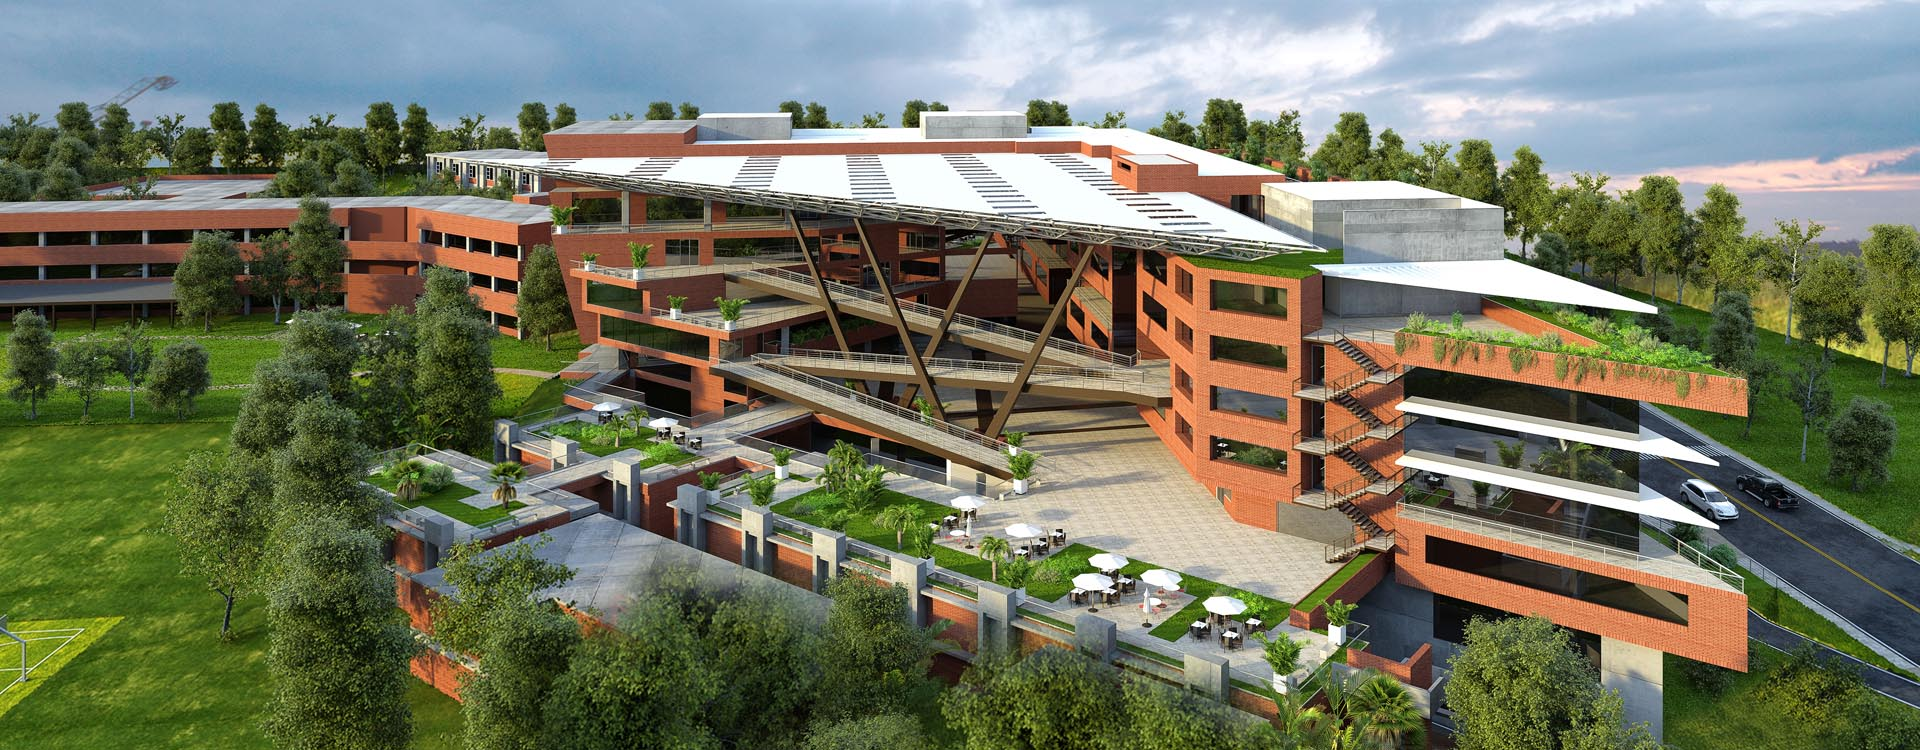
\includegraphics[height=13.25cm]{plantilla/portadacit.jpg}}
    	\makebox[\textwidth]{
    		\begin{overpic}[height=13.25cm]{\imagenportada}
     		\put(63,0){
\includegraphics[height=1.15in]{plantilla/fondologo_grande.png}}  
  			\put(64.5,2){
\includegraphics[height=0.55in]{plantilla/logoUVGblanco.eps}} 
        	\end{overpic}
    	}
    	%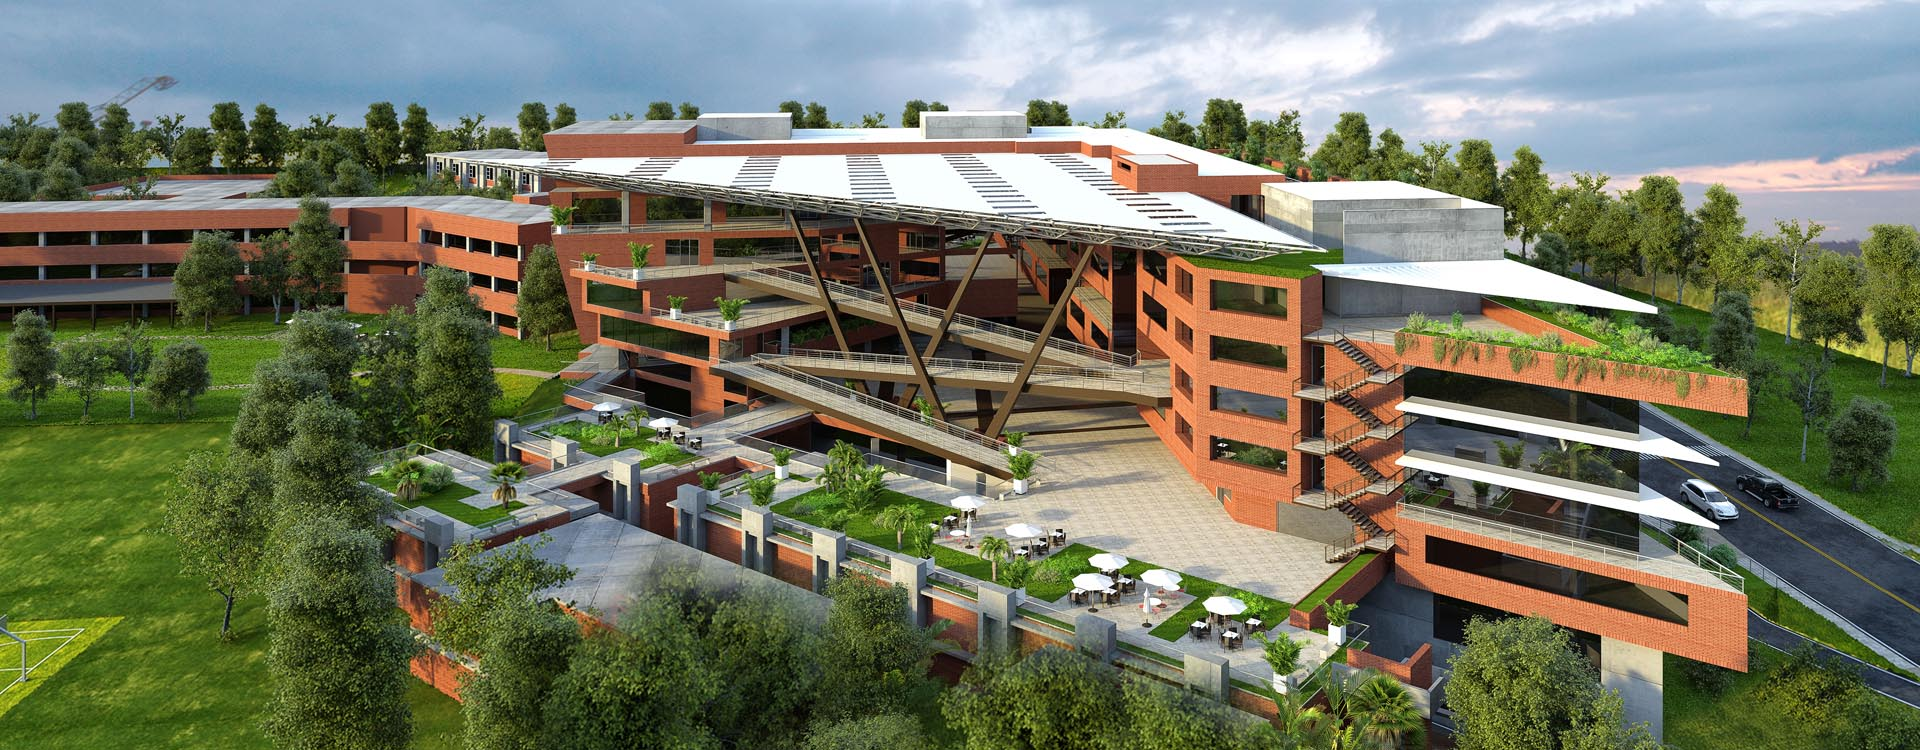
\includegraphics[height=13.25cm]{plantilla/portadacit.jpg}
	\end{figure}
	\restoregeometry
\fi

% ================================================================================
% PÁGINA EN BLANCO
% ================================================================================
\newpage
\nopagecolor
\thispagestyle{empty} % Remove page number and headers/footers

\mbox{} % Empty box to force the page to be generated

% ================================================================================
% PRIMERA PÁGINA
% ================================================================================
\ifdefined\CAPcaratula
	\newpage
%     \cleardoublepage\phantomsection
%     \pdfbookmark{Carátula}{toc}
	\pagecolor{white}
	\color{black}
	\setcounter{page}{1}
	\pagenumbering{roman}
	\thispagestyle{empty}
	\begin{center}
		\LARGE UNIVERSIDAD DEL VALLE DE GUATEMALA\\
		\LARGE Facultad de \uvgfacultad \\[0.75cm]
	\end{center}
	\begin{figure}[h]
		\begin{center}
		
\includegraphics[height=5.5 cm]{plantilla/escudoUVGcolores.eps}
		\vspace{0.5in}
		\end{center}
	\end{figure}
	\begin{center}
		\LARGE \textbf{\titulotesis} \\
		\vfill
		\vfill
		\Large Trabajo de graduación  presentado por \\
		\Large \nombreestudiante \\
		\Large para optar al grado académico de Licenciado en \uvgcarrera \\
		\vfill
		\large \quad\quad\quad\quad\quad\quad\quad\; Guatemala, \newline\newline \anoentrega
	\end{center}
\fi
% ================================================================================
% SEGUNDA PÁGINA (BLANCO)
% ================================================================================
\newpage
\thispagestyle{empty} % Remove page number and headers/footers

\mbox{} % Empty box to force the page to be generated

% ================================================================================
% TERCERA PÁGINA
% ================================================================================
\ifdefined\CAPcaratula
	\newpage
%     \cleardoublepage\phantomsection
%     \pdfbookmark{Carátula}{toc}
	\pagecolor{white}
	\color{black}
	\setcounter{page}{1}
	\pagenumbering{roman}
	\thispagestyle{empty}
	\begin{center}
		\LARGE UNIVERSIDAD DEL VALLE DE GUATEMALA\\
		\LARGE Facultad de \uvgfacultad \\[0.75cm]
	\end{center}
	\begin{figure}[h]
		\begin{center}
		
\includegraphics[height=5.5 cm]{plantilla/escudoUVGcolores.eps}
		\vspace{0.5in}
		\end{center}
	\end{figure}
	\begin{center}
		\LARGE \textbf{\titulotesis} \\
		\vfill
		\vfill
		\Large Trabajo de graduación  presentado por \\
		\Large \nombreestudiante \\
		\Large para optar al grado académico de Licenciado en \uvgcarrera \\
		\vfill
		\large \quad\quad\quad\quad\quad\quad\quad\; Guatemala, \newline\newline \anoentrega
	\end{center}
\fi
% 
% ================================================================================
% HOJA DE FIRMAS
% ================================================================================
\ifdefined\CAPfirmas
	% \newpage
	% \thispagestyle{empty}
	% \vspace*{0.5in}
	% \large Vo.Bo.:\\[1cm]
	% \begin{center}
	% 	(f) \rule[1pt]{4 in}{1pt}\\
	% 	\nombreasesor
	% \end{center}
	% \vspace{1in}

	% Tribunal Examinador:\\[1cm]
	% \begin{center}
	% 	(f) \rule[1pt]{4 in}{1pt}\\
	% 	\nombreasesor \\[1in]
	% 	(f) \rule[1pt]{4 in}{1pt}\\
	% 	\nombreprimerex \\[1in]
	% 	(f) \rule[1pt]{4 in}{1pt}\\
	% 	\nombresegundoex
	% \end{center}
	% \vspace{1in}

 %        Fecha de aprobación: Guatemala, \fechaaprobacion.
    \normalsize

    \IfFileExists{Hoja_De_Firmas_Completa_Tesis.pdf}{
        \includepdf[pages=-]{Hoja_De_Firmas_Completa_Tesis.pdf}
    }{
        \PackageWarning{tesis}{Hoja firmada pendiente de incorporar}
    }
\fi


% ================================================================================
% CONTENIDO DEL TRABAJO
% ================================================================================
% PREFACIO
% --------------------------------------------------------------------------------
\ifdefined\CAPprefacio
	\newpage
	\cleardoublepage\phantomsection
    \chapter*{Prefacio}
    \ifdefined\parpordefecto
    	\defaultparformat{prefacio}
    \else
    	% Se reservó este archivo para el prefacio personal del autor.
% No se incorporaron agradecimientos ni experiencias no proporcionados por el autor.

    \fi
    \addcontentsline{toc}{chapter}{Prefacio}
\fi

% ÍNDICE GENERAL
% --------------------------------------------------------------------------------
\ifdefined\CAPindice
	\newpage
    %\cleardoublepage\phantomsection
	\renewcommand{\contentsname}{Índice}
    \phantomsection
    \pdfbookmark{\contentsname}{toc}
	\tableofcontents
\fi

% LISTADO DE FIGURAS
% --------------------------------------------------------------------------------
\renewcommand{\listfigurename}{Lista de figuras}
\ifdefined\CAPfiguras
    \phantomsection
    \listoffigures
    \addcontentsline{toc}{chapter}{Lista de figuras}
\fi


% LISTADO DE CUADROS
% --------------------------------------------------------------------------------
%\ifdefined\CAPcuadros
%	\newpage
%    \cleardoublepage\phantomsection
% 	\renewcommand{\listtablename}{Lista de Cuadros}
% 	\listoftables
%    \chapter*{Lista de cuadros}
%    	\ifdefined\parpordefecto
%    		\defaultparformat{lista_cuadros}
%    	\else
%    		\input{lista_cuadros}
%    	\fi
%	\addcontentsline{toc}{chapter}{Lista de cuadros}
%\fi
\renewcommand{\listtablename}{Lista de cuadros}
\ifdefined\parpordefecto
    \phantomsection
    \listoftables
    \addcontentsline{toc}{chapter}{Lista de cuadros}
\fi

% RESUMEN
% --------------------------------------------------------------------------------
\ifdefined\CAPresumen
	\newpage
    \cleardoublepage\phantomsection
	\chapter*{Resumen}
	\ifdefined\parpordefecto
		\defaultparformat{resumen}
	\else
		Se estudió numéricamente la atenuación y el balance energético local de un monopolo inmerso en vacío, concreto, agua salada y tejido muscular a 3 GHz. Se empleó Meep mediante Python, con FDTD y simetría cilíndrica. Se analizaron diez configuraciones de atenuación y cinco corridas de balance. La comparación principal se efectuó a 5 px/mm; el refinamiento se examinó con las resoluciones adicionales disponibles.

Las atenuaciones aparentes a 5 px/mm fueron 0.0380, 0.7012 y 0.4669 dB/mm en concreto, agua salada y músculo, con intervalos condicionales del 95\,\% de $[0.0380,0.0381]$, $[0.7005,0.7019]$ y $[0.4663,0.4674]$ dB/mm. Las discrepancias teóricas fueron 1.31\,\%, 4.29\,\% y 5.12\,\%, respectivamente. El ajuste en vacío incumplió el criterio de calidad. En agua salada, la discrepancia se redujo a aproximadamente 0.81\,\% a 40 px/mm; el cambio de modelo y del orden aparente limitó la extrapolación al continuo.

En los anillos analizados a 5 px/mm se disipó el 81.17\,\% de la entrada en agua salada, el 74.53\,\% en músculo y el 30.38\,\% en concreto. La conductividad nula del vacío impuso una pérdida de Joule igual a cero. Los residuos finales fueron inferiores al 0.055\,\% de la entrada total. Al refinar agua salada a 10 px/mm, la fracción disipada varió un 0.4181\,\%, mientras las potencias absolutas cambiaron cerca del 30\,\%. Por ello, el cierre energético no se interpretó como convergencia de todas las magnitudes.

Se documentó un procedimiento reproducible y se delimitó su utilidad para describir pérdidas radiales relativas. La predicción de transmisión a través de interfaces y su validación con datos independientes quedaron fuera de la evidencia obtenida.

\noindent\textbf{Palabras clave:} FDTD, Meep, vector de Poynting, atenuación, balance energético, incertidumbre numérica.

	\fi
	\addcontentsline{toc}{chapter}{Resumen}
\fi

% INTRODUCCIÓN
% --------------------------------------------------------------------------------
\ifdefined\CAPintroduccion
	\newpage
	\pagenumbering{arabic}
	\setcounter{page}{1}
	\chapter{Introducción}
	\ifdefined\parpordefecto
		\defaultparformat{introduccion}
	\else
		La propagación electromagnética en un medio con pérdidas se estudió mediante la evolución de los campos y el transporte de energía. Para una antena inmersa, la disminución de la señal dependió de la expansión geométrica, la absorción del material y la distribución espacial del campo. El vector de Poynting proporcionó una relación entre estas magnitudes y la conservación de energía \citep{Griffiths2017,Poynting1884}.

En este trabajo se implementó una simulación en Python con el motor FDTD Meep a 3 GHz. Se representó un monopolo en coordenadas cilíndricas axisimétricas y se consideraron cuatro medios homogéneos: vacío, concreto, agua salada y tejido muscular. La frecuencia situó el estudio en el intervalo sub-6 GHz; no se simuló una red 5G, su modulación ni un enlace completo entre transmisor y receptor.

El análisis reunió dos conjuntos de evidencia. Diez configuraciones permitieron comparar perfiles radiales de potencia y estimar una atenuación aparente. Cinco corridas adicionales evaluaron el balance entre flujo entrante, flujo saliente y disipación de Joule en un volumen anular sin fuentes. La comparación principal se realizó a 5 px/mm. Las resoluciones adicionales permitieron examinar la aproximación a la teoría y la sensibilidad a la malla.

Se distinguieron la incertidumbre condicional del ajuste, la discrepancia respecto de la teoría, la variación entre discretizaciones y el residuo energético. Esta separación evitó interpretar un intervalo estrecho o un buen cierre del balance como demostración suficiente de exactitud. Los códigos, los registros y las figuras se organizaron para conservar la trazabilidad de cada resultado.

El alcance se limitó a la propagación dentro de cada medio, con geometrías escaladas mediante su longitud de onda. No se midió transmisión a través de paredes o interfaces, ni se estimó la eficiencia global de una antena calibrada. La discusión evaluó el cumplimiento de los objetivos dentro de estas condiciones y delimitó las verificaciones necesarias para extender el modelo.

	\fi
\fi

% OBJETIVOS
% --------------------------------------------------------------------------------
\ifdefined\CAPobjetivos
	\newpage
	\chapter{Objetivos}
	\ifdefined\parpordefecto
		\defaultparformat{objetivos}
	\else
		

\section{Objetivo general}
Realizar una simulación utilizando el lenguaje de programación Python para poder predecir por medio de métodos numéricos la atenuación por penetración de antenas utilizadas en telecomunicaciones.

\section{Objetivos específicos}
\begin{itemize}
\item Realizar una simulación que permita predecir las pérdidas de señal por penetración en distintos materiales.
\item Proponer una forma estándar de medición de las pérdidas por medio de métodos numéricos.
\item Evaluar si los resultados del modelo más simple que se utiliza en la simulación pueden utilizarse para ajustar modelos de propagación de antenas.

\end{itemize}
\section{Alcance operativo de los objetivos}
Se consideraron medios homogéneos, isótropos y no magnéticos a 3 GHz. Los parámetros de permitividad y conductividad se tomaron del programa original y se trataron como entradas del modelo; no se midieron muestras físicas ni se cuantificó la variabilidad de dichas propiedades.

La atenuación se estimó en ventanas radiales declaradas. El balance se evaluó en un anillo sin fuentes, separado del conductor y de las fronteras absorbentes. Las comparaciones describieron las configuraciones simuladas, con la longitud del monopolo y el dominio escalados por la longitud de onda de cada medio.

No se resolvieron interfaces entre dos medios de propagación, heterogeneidad interna, anisotropía, calentamiento, SAR calibrada, impedancia de entrada, patrón de radiación completo ni eficiencia global. Tampoco se efectuó una validación experimental o contra datos independientes de enlaces. Estas limitaciones se retomaron al evaluar los objetivos en la discusión.


	\fi
\fi

% JUSTIFICACIÓN
% --------------------------------------------------------------------------------
\ifdefined\CAPjustificacion
	\newpage
	\chapter{Justificación}
	\ifdefined\parpordefecto
		\defaultparformat{justificacion}
	\else
		El análisis del flujo electromagnético permitió relacionar la disminución de una señal con la energía transportada y disipada en el material. Esta relación resultó pertinente para estudiar antenas inmersas, donde la atenuación del medio y la distribución del campo influyeron simultáneamente en la potencia observada.

La simulación FDTD permitió resolver los campos de una geometría finita y contrastarlos con la referencia de onda plana. Se empleó Meep por su formulación documentada, su interfaz de Python y su soporte de coordenadas cilíndricas \citep{Yee1966,Oskooi2010}. La simetría axial redujo el costo respecto de representar explícitamente la dirección azimutal; no se midió una aceleración frente a una simulación cartesiana 3D.

La contribución consistió en integrar la estimación de atenuación, sus controles de ajuste y una comprobación independiente del balance local. Se compararon los medios a una resolución común y se cuantificaron las limitaciones mediante refinamiento, variación temporal y registros de recursos. La conservación de archivos y versiones permitió revisar el procedimiento y reproducir los cálculos derivados.

La utilidad para telecomunicaciones se interpretó como una base física y numérica para estudios posteriores. Los resultados no constituyeron una caracterización de materiales medidos, una certificación de exposición ni un modelo validado de cobertura 5G. La selección de parámetros homogéneos a una frecuencia y el escalado geométrico delimitaron las conclusiones.

	\fi
\fi

% MARCO TEÓRICO
% --------------------------------------------------------------------------------
\ifdefined\CAPmarcoteorico
	\newpage
	\chapter{Marco teórico}
	\ifdefined\parpordefecto
		\defaultparformat{marco_teorico}
	\else
		%==================================================================
\section{Fundamentos del Electromagnetismo}

\subsection{Electromagnetismo}
Durante buena parte del siglo XVIII y comienzos del XIX, la electricidad y el magnetismo se estudiaron como fenómenos independientes. En 1820 Hans Christian Ørsted observó que una corriente eléctrica desviaba la aguja de una brújula cercana, demostrando por primera vez una conexión física entre corrientes eléctricas y efectos magnéticos. A partir de esta observación, André Marie Ampère formuló durante la década de 1820 las leyes cuantitativas que describieron la fuerza entre corrientes eléctricas, sentando las bases de la electrodinámica como disciplina matemática \cite{Hon2020}.

Una década más tarde, Michael Faraday llevó a cabo los experimentos que establecieron la inducción electromagnética. Mostró que un campo magnético variable en el tiempo podía inducir una corriente eléctrica en un circuito cercano, incluso en ausencia de contacto físico o de baterías. Aunque no empleaba el lenguaje matemático formal, introdujo la noción de ``líneas de fuerza'' para representar el campo como una entidad física distribuida en el espacio y no únicamente como una abstracción utilizada para calcular fuerzas a distancia \cite{Hon2020}.

James Clerk Maxwell reunió las leyes empíricas de Coulomb, Gauss, Ampère y Faraday y, entre 1861 y 1865, las expresó mediante el cálculo diferencial. Durante este proceso identificó una inconsistencia matemática en la ley de Ampère cuando se aplicaba a situaciones no estacionarias, como la carga de un capacitor. Para resolverla introdujo un término adicional, \textbf{la corriente de desplazamiento}, con el cual se recuperó la consistencia matemática de la teoría. La formulación resultante predijo además la existencia de ondas electromagnéticas autopropagantes cuya velocidad, calculada a partir de constantes eléctricas y magnéticas medidas en el laboratorio, coincidía con la velocidad de la luz conocida experimentalmente. A partir de esta coincidencia, Maxwell concluyó que la luz correspondía a una onda electromagnética y reunió la electricidad, el magnetismo y la óptica dentro de una misma teoría de campos \cite{Hon2020}.

Heinrich Hertz confirmó experimentalmente la existencia de estas ondas entre 1887 y 1888, aproximadamente veinte años después de la formulación teórica de Maxwell, al generar y detectar ondas de radio en el laboratorio. La forma vectorial compacta de las cuatro relaciones que posteriormente se conocieron como ecuaciones de Maxwell no fue escrita por el propio Maxwell, quien había trabajado con un conjunto mayor de ecuaciones expresadas por componentes. Esta formulación se debió a la posterior reorganización de Oliver Heaviside mediante el cálculo vectorial moderno. La distinción resultó relevante porque las herramientas de divergencia, rotacional y teoremas integrales utilizadas para pasar entre las formas integral y diferencial, y posteriormente para construir el esquema de Yee, correspondieron a una formalización posterior de los descubrimientos físicos originales \cite{Fumeron2020}.

\section{Electricidad y campo eléctrico}

\subsection{Carga eléctrica y campo eléctrico}
La carga eléctrica $q$ fue la propiedad fundamental de la materia responsable de la interacción electromagnética. Se consideraron dos signos de carga: las cargas de signo igual se repelían, mientras que las de signo opuesto se atraían. El campo eléctrico $\vec{E}(\vec{r})$ en un punto del espacio se definió como la fuerza por unidad de carga que experimentaría una carga de prueba $q_0$ infinitesimalmente pequeña (para no perturbar la distribución de carga que generó el campo) colocada en dicho punto:
\begin{equation}
    \vec{E}(\vec{r}) \equiv \lim_{q_0 \to 0} \frac{\vec{F}(\vec{r})}{q_0}
\end{equation}
Esta definición convirtió al campo eléctrico en una propiedad asociada al espacio y a la distribución de cargas que lo producía, independiente de la carga de prueba utilizada para medirlo. De esta manera, el campo pudo tratarse como una entidad física definida en cada punto del espacio \cite{Griffiths2017}.

\subsection{Ley de Coulomb}
La ley de Coulomb, establecida experimentalmente por Charles Augustin de Coulomb en 1785 mediante una balanza de torsión, cuantificó la fuerza electrostática entre dos cargas puntuales $q_1$ y $q_2$ separadas una distancia $r$:
\begin{equation}
    \vec{F}_{12} = \frac{1}{4\pi\varepsilon_0} \frac{q_1 q_2}{r^2} \hat{r}
\end{equation}
donde $\hat{r}$ fue el vector unitario que apuntaba de la carga fuente hacia el punto de observación y $\varepsilon_0 \approx 8.854 \times 10^{-12} \text{ F/m}$ fue la permitividad eléctrica del vacío. La constante $k = 1 / 4\pi\varepsilon_0 \approx 8.988 \times 10^9 \text{ N}\cdot\text{m}^2/\text{C}^2$ se conoció como constante de Coulomb. A partir de esta ley y de la definición de campo eléctrico, el campo generado por una carga puntual $q$ en el origen fue:
\begin{equation}
    \vec{E}(\vec{r}) = \frac{1}{4\pi\varepsilon_0} \frac{q}{r^2} \hat{r}
\end{equation}
Debido a que las fuerzas eléctricas obedecían el principio de superposición (la fuerza neta sobre una carga de prueba debida a varias fuentes fue la suma vectorial de las fuerzas individuales), el campo generado por una distribución continua de carga con densidad volumétrica $\rho(\vec{r}')$ contenida en un volumen $V$ se obtuvo integrando las contribuciones infinitesimales $dq' = \rho(\vec{r}') \, dV'$:
\begin{equation}
    \vec{E}(\vec{r}) = \frac{1}{4\pi\varepsilon_0} \int_V \rho(\vec{r}') \frac{\vec{r} - \vec{r}'}{|\vec{r} - \vec{r}'|^3} \, dV'
\end{equation}
Esta forma integral podía resultar difícil de evaluar directamente para distribuciones de carga complejas. La ley de Gauss proporcionó una relación alternativa entre el campo y sus fuentes y, por ello, resultó útil como base para las formulaciones diferenciales utilizadas posteriormente.

\subsection{Ley de Gauss para el campo eléctrico}
\textbf{Forma integral.} Se consideró una carga puntual $q$ situada en el centro de una superficie esférica de radio $r$. Como $\vec{E}$ era radial y su magnitud permanecía constante sobre la esfera, el flujo se escribió como:
\begin{equation}
    \oint_S \vec{E} \cdot d\vec{A} = \frac{1}{4\pi\varepsilon_0} \frac{q}{r^2} (4\pi r^2) = \frac{q}{\varepsilon_0}
\end{equation}
El resultado fue independiente del radio $r$: todo el flujo generado por la carga atravesaba cualquier esfera que la encerrara. Un argumento de ángulo sólido permitió generalizar el resultado a una superficie cerrada de forma arbitraria, y el principio de superposición permitió extenderlo a una distribución arbitraria de cargas. Se obtuvo así la \textit{ley de Gauss} en su forma integral:
\begin{equation}
    \oint_S \vec{E} \cdot d\vec{A} = \frac{Q_{\text{enc}}}{\varepsilon_0}
\end{equation}
donde $Q_{\text{enc}}$ fue la carga neta encerrada por la superficie cerrada $S$.

\textbf{Forma diferencial.} Si se escribió $Q_{\text{enc}} = \int_V \rho \, dV$ y se aplicó el teorema de la divergencia (teorema de Gauss y Ostrogradsky) al miembro izquierdo:
\begin{equation}
    \oint_S \vec{E} \cdot d\vec{A} = \int_V \nabla \cdot \vec{E} \, dV = \int_V \frac{\rho}{\varepsilon_0} \, dV
\end{equation}
Como esta igualdad debía cumplirse para cualquier volumen $V$ elegido arbitrariamente, los integrandos debían ser iguales punto a punto, lo que condujo a la forma diferencial (local) de la ley de Gauss:
\begin{equation}
    \nabla \cdot \vec{E} = \frac{\rho}{\varepsilon_0}
\end{equation}

\textbf{Interpretación física.} La forma diferencial relacionó directamente la densidad de carga con la divergencia del campo eléctrico. En regiones con carga positiva, las líneas de campo divergían; con carga negativa, convergían. En regiones sin carga se cumplía $\nabla \cdot \vec{E}=0$. Esta relación correspondió a la primera ecuación de Maxwell y, dentro de una formulación discreta consistente, quedó vinculada con la conservación de la carga mediante la ley de Ampère con la corrección de Maxwell y la ecuación de continuidad \cite{Taflove2005}.

\section{Magnetismo y campo magnético}

\subsection{Fuerza magnética y campo magnético}
A diferencia del campo eléctrico, no existían cargas magnéticas aisladas, \textbf{monopolos magnéticos}, en la naturaleza observada; el magnetismo se originaba en cargas eléctricas en movimiento llamadas \textbf{corrientes}. El campo magnético $\vec{B}$ se definió a través de la fuerza que ejercía sobre una carga de prueba $q$ que se movía con velocidad $\vec{v}$, dada por la fuerza de Lorentz:
\begin{equation}
    \vec{F} = q(\vec{v} \times \vec{B})
\end{equation}
Se observó que esta fuerza fue siempre perpendicular a la velocidad de la carga, por lo que un campo magnético estático no realizaba trabajo sobre una carga en movimiento; únicamente modificaba la dirección de su velocidad.

\subsection{Ley de Gauss para el campo magnético}
La ausencia experimental de monopolos magnéticos se expresó mediante la condición de que el flujo magnético neto a través de cualquier superficie cerrada fuera nulo:
\begin{equation}
    \oint_S \vec{B} \cdot d\vec{A} = 0
\end{equation}
Al aplicar el teorema de la divergencia y exigir que la igualdad se cumpliera para cualquier volumen, se obtuvo la forma diferencial:
\begin{equation}
    \nabla \cdot \vec{B} = 0
\end{equation}
Esta relación correspondió a la segunda ecuación de Maxwell. Desde el punto de vista físico, indicó que el campo magnético era solenoidal: sus líneas no presentaban un inicio o un final aislado, sino que formaban trayectorias cerradas. En el algoritmo de Yee, esta condición se preservó de manera natural por la geometría escalonada de la malla, una propiedad relevante del método \cite{Teixeira2023}.

\subsection{Ley de Ampère}
La ley de Ampère, formulada a partir de los experimentos de Ørsted y del propio Ampère en la década de 1820, relacionó la circulación del campo magnético alrededor de una trayectoria cerrada con la corriente eléctrica que atravesaba cualquier superficie delimitada por dicha trayectoria:
\begin{equation}
    \oint_C \vec{B} \cdot d\vec{\ell} = \mu_0 I_{\text{enc}}
\end{equation}
donde $\mu_0 = 4\pi \times 10^{-7} \text{ T}\cdot\text{m/A}$ fue la permeabilidad magnética del vacío e $I_{\text{enc}}$ fue la corriente neta que atravesaba cualquier superficie $S$ cuyo borde fuera la curva $C$. Escribiendo $I_{\text{enc}} = \int_S \vec{J} \cdot d\vec{A}$, donde $\vec{J}$ fue la densidad de corriente, y aplicando el teorema de Stokes al miembro izquierdo:
\begin{equation}
    \oint_C \vec{B} \cdot d\vec{\ell} = \int_S (\nabla \times \vec{B}) \cdot d\vec{A} = \mu_0 \int_S \vec{J} \cdot d\vec{A}
\end{equation}
Como la superficie $S$ fue arbitraria (cualquier superficie que tuviera a $C$ como borde debía dar el mismo resultado), se obtuvo la forma diferencial de la ley de Ampère en su versión original, válida solo para corrientes estacionarias:
\begin{equation}
    \nabla \times \vec{B} = \mu_0 \vec{J}
\end{equation}
Como se mostró previamente al analizar la corrección introducida por Maxwell, esta expresión resultó incompleta y debía corregirse para dar cuenta de situaciones no estacionarias.

\section{Ley de Faraday: inducción electromagnética}
Los experimentos de Faraday de 1831 mostraron que una fuerza electromotriz (f.e.m.) se inducía en un circuito cerrado cuando el flujo magnético $\Phi_B = \int_S \vec{B} \cdot d\vec{A}$ a través de una superficie delimitada por el circuito variaba en el tiempo, sin importar si dicha variación se debía al movimiento del circuito, del imán, o a un cambio intrínseco del campo. La ley de Faraday, en su forma integral, estableció:
\begin{equation}
    \oint_C \vec{E} \cdot d\vec{\ell} = -\frac{d\Phi_B}{dt} = -\frac{d}{dt} \int_S \vec{B} \cdot d\vec{A}
\end{equation}
El signo negativo representó la ley de Lenz: la fuerza electromotriz inducida se oponía a la variación de flujo que la originaba, garantizando la conservación de la energía. Suponiendo una superficie fija en el tiempo (de modo que la derivada temporal podía introducirse dentro de la integral) y aplicando el teorema de Stokes al miembro izquierdo:
\begin{equation}
    \int_S (\nabla \times \vec{E}) \cdot d\vec{A} = - \int_S \frac{\partial \vec{B}}{\partial t} \cdot d\vec{A}
\end{equation}
de donde, al ser $S$ arbitraria, se obtuvo la forma diferencial:
\begin{equation}
    \nabla \times \vec{E} = -\frac{\partial \vec{B}}{\partial t}
\end{equation}
Esta relación correspondió a la tercera ecuación de Maxwell. Físicamente, indicó que un campo magnético variable en el tiempo generaba un campo eléctrico rotacional. Junto con la corrección introducida por Maxwell en la ley de Ampère, este acoplamiento permitió explicar cómo una perturbación electromagnética podía sostenerse y propagarse en una región sin cargas ni corrientes libres, como se desarrolló posteriormente.

\section{La inconsistencia de Ampère y la corrección de Maxwell: la corriente de desplazamiento}
La forma diferencial de la ley de Ampère obtenida previamente, $\nabla \times \vec{B} = \mu_0 \vec{J}$, fue matemáticamente inconsistente en el caso general. Para comprobarlo, se tomó la divergencia de ambos miembros. La divergencia del rotacional de cualquier campo vectorial fue idénticamente nula:
\begin{equation}
    \nabla \cdot (\nabla \times \vec{B}) \equiv 0 \implies \mu_0 \nabla \cdot \vec{J} = 0 \implies \nabla \cdot \vec{J} = 0
\end{equation}
Sin embargo, la conservación de la carga eléctrica se expresó mediante la ecuación de continuidad,
\begin{equation}
    \nabla \cdot \vec{J} = -\frac{\partial \rho}{\partial t}
\end{equation}
que estableció que la corriente que divergía de un punto debía ser igual a la rapidez con que decrecía la densidad de carga en ese punto. La ley de Ampère original exigió $\nabla \cdot \vec{J} = 0$ en todo momento, lo cual solo fue cierto si $\partial \rho / \partial t = 0$, es decir, únicamente en régimen estacionario (corriente continua, sin acumulación de carga en ningún punto). 

En una situación tan elemental como la carga de un capacitor, donde la corriente de conducción $\vec{J}$ se interrumpía físicamente entre las placas, la ley de Ampère original conducía a una contradicción: el valor de $I_{\text{enc}}$ calculado con la ley de Ampère dependía de qué superficie se eligiera para delimitar la curva $C$, violando la condición de que dicho valor debía ser independiente de la superficie escogida.

Maxwell resolvió esta inconsistencia postulando la existencia de un término adicional, la \textit{corriente de desplazamiento}, definida como:
\begin{equation}
    \vec{J}_d \equiv \varepsilon_0 \frac{\partial \vec{E}}{\partial t}
\end{equation}
Para verificar que este término restauraba la consistencia, se utilizó la ley de Gauss ($\rho = \varepsilon_0 \nabla \cdot \vec{E}$) y se reescribió la ecuación de continuidad:
\begin{equation}
    \frac{\partial \rho}{\partial t} = \varepsilon_0 \frac{\partial}{\partial t} (\nabla \cdot \vec{E}) = \nabla \cdot \left( \varepsilon_0 \frac{\partial \vec{E}}{\partial t} \right)
\end{equation}
de modo que la ecuación de continuidad podía escribirse como $\nabla \cdot \vec{J} + \nabla \cdot \vec{J}_d = 0$, es decir, $\nabla \cdot (\vec{J} + \vec{J}_d) = 0$.

Maxwell propuso entonces sustituir $\vec{J}$ por $\vec{J} + \vec{J}_d$ en la ley de Ampère, obteniendo la \textit{ley de Ampère con la corrección de Maxwell}:
\begin{equation}
    \nabla \times \vec{B} = \mu_0 \vec{J} + \mu_0 \varepsilon_0 \frac{\partial \vec{E}}{\partial t}
\end{equation}
Esta forma sí fue consistente: al tomar su divergencia se obtuvo $0 = \mu_0 \nabla \cdot (\vec{J} + \vec{J}_d)$, que fue idénticamente cierto por la ecuación de continuidad, en cualquier régimen, estacionario o no. 

En el ejemplo del capacitor, la corriente de desplazamiento entre las placas estuvo asociada con el campo eléctrico variable presente en esa región, aunque no existiera una corriente de conducción real entre las placas. Este término sustituyó a la corriente de conducción que faltaba cuando se elegía una superficie que pasaba por el espacio entre placas, de modo que $I_{\text{enc}}$ dejó de depender de la superficie escogida.

Esta corrección, aparentemente un detalle técnico para resolver una inconsistencia matemática, fue la que introdujo el acoplamiento bidireccional entre $\vec{E}$ y $\vec{B}$ que hizo posible la propagación ondulatoria: un campo eléctrico variable generó un campo magnético (mediante la ley de Ampère con la corrección de Maxwell), y un campo magnético variable generó un campo eléctrico (vía Faraday), permitiendo que la perturbación se autosostuviera y viajara por el espacio sin necesidad de un medio material ni de cargas libres. También fue el término de desplazamiento el que se discretizó en la malla de Yee para obtener la ecuación de actualización temporal del campo eléctrico \cite{Yee1966, Taflove2005}.

\section{Las ecuaciones de Maxwell: síntesis unificada}
Reuniendo los resultados de los apartados anteriores, las cuatro ecuaciones de Maxwell en el vacío, en presencia de fuentes libres $\rho$ y $\vec{J}$, fueron:

\textbf{Forma diferencial (local):}
\begin{table}[htbp]
    \centering
    \renewcommand{\arraystretch}{1.5}
    \begin{tabular}{ll}
        \hline
        \textbf{Nombre} & \textbf{Ecuación} \\
        \hline
        Ley de Gauss (eléctrica) & $\nabla \cdot \vec{E} = \frac{\rho}{\varepsilon_0}$ \\
        Ley de Gauss (magnética) & $\nabla \cdot \vec{B} = 0$ \\
        Ley de Faraday & $\nabla \times \vec{E} = -\frac{\partial \vec{B}}{\partial t}$ \\
        Ley de Ampère con la corrección de Maxwell & $\nabla \times \vec{B} = \mu_0 \vec{J} + \mu_0 \varepsilon_0 \frac{\partial \vec{E}}{\partial t}$ \\
        \hline
    \end{tabular}
    \caption{Ecuaciones de Maxwell en el vacío en forma diferencial.}
    \label{tab:maxwell_diferencial}
\end{table}

\textbf{Forma integral:}
\begin{align}
    \oint_S \vec{E} \cdot d\vec{A} &= \frac{Q_{\text{enc}}}{\varepsilon_0}, & \oint_S \vec{B} \cdot d\vec{A} &= 0 \\
    \oint_C \vec{E} \cdot d\vec{\ell} &= -\frac{d}{dt} \int_S \vec{B} \cdot d\vec{A}, & \oint_C \vec{B} \cdot d\vec{\ell} &= \mu_0 I_{\text{enc}} + \mu_0 \varepsilon_0 \frac{d}{dt} \int_S \vec{E} \cdot d\vec{A}
\end{align}

Para un medio material lineal, homogéneo e isótropo, la aproximación que se empleó para cada uno de los medios complejos considerados en esta tesis (concreto, agua salada, tejido muscular, etc.), fue conveniente introducir el desplazamiento eléctrico $\vec{D} = \varepsilon \vec{E}$ y el campo magnético auxiliar $\vec{H} = \vec{B}/\mu$, con $\varepsilon = \varepsilon_r \varepsilon_0$ y $\mu = \mu_r \mu_0$ las constantes del medio. 

Las ecuaciones de Maxwell ``macroscópicas'' tomaron entonces una forma que permitió describir los medios materiales y que, además, constituyó la base directa de la implementación FDTD:
\begin{equation}
    \nabla \cdot \vec{D} = \rho_{\text{libre}}, \quad \nabla \cdot \vec{B} = 0, \quad \nabla \times \vec{E} = -\frac{\partial \vec{B}}{\partial t}, \quad \nabla \times \vec{H} = \vec{J}_{\text{libre}} + \frac{\partial \vec{D}}{\partial t}
\end{equation}
Esta síntesis, cuatro ecuaciones acopladas de primer orden en el tiempo y el espacio, fue, en el sentido más literal, el objeto matemático que un simulador FDTD como MEEP resolvía numéricamente en cada celda de la malla y en cada paso temporal \cite{Teixeira2023}.

\section{De las ecuaciones de Maxwell a la ecuación de onda electromagnética}
A continuación se dedujo el resultado que conectó las ecuaciones de Maxwell con la propagación ondulatoria: la existencia de ondas electromagnéticas y la relación que determinaba su velocidad.

\textbf{Paso 1, Región sin fuentes.} Se consideró una región del espacio sin cargas ni corrientes libres ($\rho = 0$, $\vec{J} = 0$), como la región que rodeaba a una antena lejos de sus conductores. Bajo esta condición, las ecuaciones de Maxwell se redujeron a:
\begin{equation}
    \nabla \cdot \vec{E} = 0, \quad \nabla \cdot \vec{B} = 0, \quad \nabla \times \vec{E} = -\frac{\partial \vec{B}}{\partial t}, \quad \nabla \times \vec{B} = \mu_0 \varepsilon_0 \frac{\partial \vec{E}}{\partial t}
\end{equation}

\textbf{Paso 2, Desacoplar las ecuaciones.} Se tomó el rotacional de la ley de Faraday:
\begin{equation}
    \nabla \times (\nabla \times \vec{E}) = -\frac{\partial}{\partial t} (\nabla \times \vec{B})
\end{equation}
Sustituyendo en el miembro derecho la ley de Ampère con la corrección de Maxwell (sin fuentes):
\begin{equation}
    \nabla \times (\nabla \times \vec{E}) = -\mu_0 \varepsilon_0 \frac{\partial^2 \vec{E}}{\partial t^2}
\end{equation}

\textbf{Paso 3, Identidad vectorial.} Se empleó la identidad del cálculo vectorial
\begin{equation}
    \nabla \times (\nabla \times \vec{E}) = \nabla(\nabla \cdot \vec{E}) - \nabla^2 \vec{E}
\end{equation}
y, como en la región considerada $\nabla \cdot \vec{E}=0$ (Paso 1), el primer término se anuló, por lo que quedó:
\begin{equation}
    -\nabla^2 \vec{E} = -\mu_0 \varepsilon_0 \frac{\partial^2 \vec{E}}{\partial t^2}
\end{equation}

\textbf{Paso 4, Ecuación de onda.} Reordenando, se obtuvo la ecuación de onda vectorial homogénea para el campo eléctrico:
\begin{equation}
    \nabla^2 \vec{E} - \mu_0 \varepsilon_0 \frac{\partial^2 \vec{E}}{\partial t^2} = 0
\end{equation}
y, mediante un procedimiento idéntico partiendo de la ley de Ampère con la corrección de Maxwell y sustituyendo la ley de Faraday, se obtuvo la ecuación análoga para el campo magnético:
\begin{equation}
    \nabla^2 \vec{B} - \mu_0 \varepsilon_0 \frac{\partial^2 \vec{B}}{\partial t^2} = 0
\end{equation}

\textbf{Interpretación física.} Ambas ecuaciones tenían la forma canónica de una ecuación de onda tridimensional, $\nabla^2 \psi - \frac{1}{v^2} \frac{\partial^2 \psi}{\partial t^2} = 0$, cuya velocidad de propagación fue
\begin{equation}
    v = \frac{1}{\sqrt{\mu_0 \varepsilon_0}}
\end{equation}
Al sustituir los valores medidos de $\mu_0$ y $\varepsilon_0$, constantes obtenidas originalmente de experimentos puramente eléctricos y magnéticos, sin ninguna referencia a la óptica, se obtuvo $v \approx 2.998 \times 10^8 \text{ m/s} = c$, la velocidad de la luz en el vacío. Este resultado, obtenido por Maxwell en 1865 por vía puramente teórica y confirmado experimentalmente por Hertz veinte años después, fue el que permitió identificar a la luz visible como un caso particular de onda electromagnética, unificando la óptica con el electromagnetismo \cite{Hon2020}.

Para el desarrollo posterior de esta tesis, dos observaciones fueron cruciales:
\begin{itemize}
    \item En un medio material con pérdidas, como el agua salada, el concreto húmedo o el tejido muscular estudiados en esta tesis, las ecuaciones de Maxwell incluyeron una densidad de corriente de conducción $\vec{J}=\sigma\vec{E}$, con $\sigma$ como conductividad del medio. Al no anularse este término, el mismo procedimiento condujo a una \textit{ecuación de onda amortiguada} con un término disipativo proporcional a $\sigma \frac{\partial \vec{E}}{\partial t}$. Este resultado proporcionó la base matemática de la atenuación y de las pérdidas de potencia que posteriormente se estudiaron mediante el vector de Poynting.
    \item La deducción anterior se realizó en el continuo. En su formulación numérica, el algoritmo de Yee sustituyó los operadores diferenciales $\nabla \times$ y $\partial/\partial t$ de las ecuaciones de Ampère con la corrección de Maxwell y de Faraday por diferencias finitas centradas sobre una malla espaciotemporal escalonada. Al refinar la discretización, la evolución temporal de las ecuaciones discretizadas se aproximó a la propagación ondulatoria obtenida en el continuo \cite{Yee1966, Teixeira2023}.
\end{itemize}

\section{Ondas Electromagnéticas}

\subsection{Solución de onda plana armónica en un medio sin pérdidas}
Se buscó una solución de la ecuación de onda homogénea:
\begin{equation}
    \nabla^2\vec{E} - \mu\varepsilon\frac{\partial^2\vec{E}}{\partial t^2} = 0
\end{equation}
de la forma de una onda plana uniforme que se propagaba en la dirección $+\hat{z}$ y estaba polarizada linealmente a lo largo de $\hat{x}$:
\begin{equation}
    \vec{E}(z, t) = \text{Re}\left[E_0 e^{i(kz-\omega t)}\right]\hat{x}
\end{equation}

Al sustituir esta forma de prueba en la ecuación de onda, cada derivada espacial aportó un factor $ik$ y cada derivada temporal un factor $-i\omega$, de modo que:
\begin{equation}
    (ik)^2 E_0 e^{i(kz-\omega t)} - \mu\varepsilon(-i\omega)^2 E_0 e^{i(kz-\omega t)} = 0 \implies -k^2 + \mu\varepsilon\omega^2 = 0
\end{equation}
lo que produjo la relación de dispersión:
\begin{equation}
    k = \omega\sqrt{\mu\varepsilon} \qquad \text{(número de onda, rad/m)}
\end{equation}

Esta relación, lineal entre $k$ y $\omega$, fue la que caracterizó a un medio no dispersivo: todas las frecuencias viajaban a la misma velocidad. Cuando $\varepsilon$ o $\mu$ dependieron de la frecuencia (como ocurrió en los modelos de Debye y de Lorentz del modelo de medios considerado), la relación dejaba de ser lineal y el medio se volvió dispersivo, con consecuencias importantes sobre la forma de un pulso que se propagara en él.

El campo magnético asociado se obtuvo de la ley de Faraday, $\nabla\times\vec{E} = -\mu \frac{\partial\vec{H}}{\partial t}$. Para la onda propuesta, el rotacional se redujo a $-ikE_0 e^{i(kz-\omega t)}\hat{y}$ (dado que $\vec{E}$ solo dependió de $z$), y al igualar con $-\mu(-i\omega)\vec{H}$ se obtuvo $\vec{H}(z, t) = \text{Re}\left[H_0 e^{i(kz-\omega t)}\right]\hat{y}$, con:
\begin{equation}
    H_0 = \frac{k}{\omega\mu}E_0 = \frac{E_0}{\sqrt{\mu/\varepsilon}}
\end{equation}

Se observó que $\vec{E}$, $\vec{H}$ y la dirección de propagación $\hat{z}$ formaban un triedro ortogonal. Por esta razón, la onda electromagnética en un medio homogéneo e isótropo correspondió a una onda transversal electromagnética (TEM), sin componentes de campo en la dirección de propagación.

\section{Velocidad de fase, longitud de onda y frecuencia}
La velocidad de fase fue la rapidez con la que se desplazaba un frente de fase constante ($kz-\omega t = \text{cte.}$):
\begin{equation}
    v_p = \frac{\omega}{k} = \frac{1}{\sqrt{\mu\varepsilon}} = \frac{c}{\sqrt{\mu_r\varepsilon_r}} = \frac{c}{n}
\end{equation}
donde $n=\sqrt{\mu_r\varepsilon_r}$ fue el índice de refracción del medio \cite{ITU2025}. La longitud de onda $\lambda$, distancia espacial tras la cual la fase avanzaba $2\pi$, y la frecuencia $f$, número de oscilaciones por segundo, se relacionaron con $k$ y $\omega$ mediante:
\begin{equation}
    \lambda = \frac{2\pi}{k} = \frac{v_p}{f}, \qquad \omega = 2\pi f
\end{equation}

Un punto que tuvo relevancia para esta tesis fue el siguiente: al pasar de un medio a otro (por ejemplo, del aire al agua salada, o del aire al tejido muscular), la frecuencia de la onda, fijada por la fuente, en este caso la antena Marconi excitada a una frecuencia determinada, no cambió, pero sí lo hicieron la velocidad de fase y, en consecuencia, la longitud de onda dentro del medio, que se acortaba en un factor $1/\sqrt{\varepsilon_r}$ (en un medio con pérdidas se empleó $\lambda=2\pi/\beta$, con $\beta$ la parte real del número de onda). Este acortamiento de la longitud de onda dentro de medios de alta permitividad, el agua tenía $\varepsilon_r\approx 80$ a bajas frecuencias, tenía implicaciones prácticas directas sobre el diseño geométrico de la malla FDTD dentro de la formulación FDTD, que debía resolver espacialmente la longitud de onda más corta de entre todos los medios simulados.

\section{Impedancia intrínseca del medio}
La razón entre las amplitudes complejas del campo eléctrico y del campo magnético de una onda plana definió la impedancia intrínseca del medio:
\begin{equation}
    \eta \equiv \frac{E_0}{H_0} = \sqrt{\frac{\mu}{\varepsilon}}
\end{equation}

En el vacío se obtuvo $\eta_0=\sqrt{\mu_0/\varepsilon_0}\approx376.73\ \Omega$, cantidad conocida como impedancia del espacio libre. Para una onda plana, la impedancia intrínseca desempeñó un papel análogo al de la impedancia característica de una línea de transmisión: determinó la relación entre los campos, intervino en los coeficientes de reflexión y transmisión en una interfaz \cite[ecs.~31--38]{ITU2025} y fijó la relación entre las contribuciones eléctrica y magnética de la onda.

\section{Propagación en medios con pérdidas: atenuación y penetración}
En un medio con conductividad $\sigma\neq0$, como el concreto, el agua salada y el tejido muscular considerados en esta tesis, se repitió el procedimiento empleado previamente para la onda plana armónica, esta vez a partir de la ecuación de onda con pérdidas obtenida previamente:
\begin{equation}
    \nabla^2\vec{E} = \mu\varepsilon\frac{\partial^2\vec{E}}{\partial t^2} + \mu\sigma\frac{\partial\vec{E}}{\partial t}
\end{equation}

Al sustituir nuevamente $\vec{E}=\text{Re}[E_0 e^{i(kz-\omega t)}]\hat{x}$, cada derivada temporal aportó un factor $-i\omega$ y se obtuvo:
\begin{equation}
    -k^2 = -\omega^2\mu\varepsilon - i\omega\mu\sigma \implies k^2 = \omega^2\mu\left(\varepsilon+i\frac{\sigma}{\omega}\right) = \omega^2\mu\varepsilon_c
\end{equation}
donde $\varepsilon_c = \varepsilon + i\sigma/\omega$ fue la permitividad compleja ya introducida previamente. El número de onda pasó entonces a ser complejo; se escribió convencionalmente como:
\begin{equation}
    k = \beta + i\alpha
\end{equation}
de modo que la onda tomó la forma $E_0 e^{i\beta z} e^{-\alpha z} e^{-i\omega t}$: se propagó con fase gobernada por $\beta$ (la constante de fase, en rad/m) mientras su amplitud decaía exponencialmente según $e^{-\alpha z}$, con $\alpha$ la constante de atenuación (en Np/m). Igualando partes real e imaginaria de $k^2=\omega^2\mu\varepsilon_c$ se obtuvo el sistema:
\begin{equation}
    \beta^2-\alpha^2 = \omega^2\mu\varepsilon \qquad 2\alpha\beta = \omega\mu\sigma
\end{equation}
cuya solución simultánea produjo las expresiones estándar:
\begin{equation}
    \alpha = \omega\sqrt{\frac{\mu\varepsilon}{2}}\left[\sqrt{1+\left(\frac{\sigma}{\omega\varepsilon}\right)^2}-1\right]^{1/2} \qquad \beta = \omega\sqrt{\frac{\mu\varepsilon}{2}}\left[\sqrt{1+\left(\frac{\sigma}{\omega\varepsilon}\right)^2}+1\right]^{1/2}
\end{equation}

Estas fórmulas coincidieron, salvo por una diferencia de signo en la parte imaginaria de $\varepsilon_c$, debida únicamente a la convención temporal elegida ($e^{-i\omega t}$ en esta tesis frente a $e^{+j\omega t}$ en la convención de ingeniería utilizada por la UIT), sin modificar ninguna magnitud física, con las recomendadas directamente por la Recomendación P.2040, revisión 4 de la UIT R \cite{ITU2025} para el cálculo de atenuación en materiales de construcción.

La cantidad adimensional que aparece repetidamente, $\tan\delta = \sigma/(\omega\varepsilon)$, fue la tangente de pérdidas del medio, y resultó ser la magnitud individual más importante para clasificar el comportamiento electromagnético de un material a una frecuencia dada \cite{ITU2025}:
\begin{itemize}
    \item Si $\tan\delta \ll 1$ (medio de bajas pérdidas, ``buen dieléctrico''): $\alpha \approx \dfrac{\sigma}{2}\sqrt{\dfrac{\mu}{\varepsilon}}$, casi independiente de la frecuencia salvo por la dependencia de $\sigma$ y $\varepsilon$ con ella.
    \item Si $\tan\delta \gg 1$ (medio de altas pérdidas, ``buen conductor''): $\alpha\approx\beta\approx\sqrt{\pi f\mu\sigma}$, y ambas crecían con la raíz cuadrada de la frecuencia.
\end{itemize}

La profundidad de penetración (o ``skin depth'' cuando el medio fue un buen conductor) se definió como la distancia $\delta_p=1/\alpha$ a la cual la amplitud del campo decaía a $1/e\approx 36.8\%$ de su valor inicial. Fue habitual expresar la atenuación en decibelios por metro mediante la conversión $A\text{ [dB/m]} = 8.686\alpha\text{ [Np/m]}$ \cite[ec.~26]{ITU2025}. Estas dos cantidades, $\alpha$ (o, equivalentemente, $\delta_p$) y $\beta$, fueron, junto con la impedancia intrínseca compleja $\eta=\sqrt{\mu/\varepsilon_c}$, los tres parámetros que describieron por completo la propagación de una onda plana en cualquiera de los medios complejos estudiados en esta tesis, y fueron exactamente las cantidades que un simulador FDTD reprodujo numéricamente cuando resolvía las ecuaciones de Maxwell discretizadas en presencia de un material con pérdidas dentro de la formulación FDTD.

En un medio con pérdidas, $\vec{E}$ y $\vec{H}$ dejaban de estar en fase. La impedancia intrínseca $\eta=\sqrt{\mu/\varepsilon_c}$ adquiría un valor complejo, $\eta=|\eta|e^{i\theta_\eta}$, con $\tan(2\theta_\eta)=-\sigma/(\omega\varepsilon)$. Como consecuencia, el campo magnético presentaba un desfase $\theta_\eta$ respecto del campo eléctrico. Este desfase reducía la componente del vector de Poynting asociada con el transporte neto de potencia, mientras que parte de la energía instantánea permanecía intercambiándose entre las contribuciones eléctrica y magnética.

\section{Polarización de las ondas electromagnéticas}
Hasta ese punto se había considerado una onda con el campo eléctrico oscilando enteramente a lo largo de una única dirección transversal fija ($\hat{x}$): este fue el caso de la polarización lineal. En general, sin embargo, una onda plana que se propagó a lo largo de $\hat{z}$ podía tener simultáneamente dos componentes transversales independientes:
\begin{equation}
    \vec{E}(z, t) = \text{Re}\left[\left(E_{x0}\hat{x} + E_{y0}e^{i\phi}\hat{y}\right)e^{i(kz-\omega t)}\right]
\end{equation}
donde $E_{x0}$, $E_{y0}$ fueron reales y $\phi$ fue la diferencia de fase entre ambas componentes. Según los valores relativos de $E_{x0}$, $E_{y0}$ y $\phi$, la punta del vector $\vec{E}$, observada en un plano transversal fijo, trazaba una de tres figuras:
\begin{itemize}
    \item \textbf{Polarización lineal:} si $\phi=0$ o $\phi=\pi$ (las componentes estuvieron en fase o en contrafase), la punta del vector oscilaba a lo largo de una línea recta cuya orientación dependió del cociente $E_{y0}/E_{x0}$.
    \item \textbf{Polarización circular:} si $E_{x0}=E_{y0}$ y $\phi=\pm\pi/2$, la punta del vector describió un círculo; el signo de $\phi$ determinaba el sentido de giro (dextrógiro o levógiro, según la convención del IEEE).
    \item \textbf{Polarización elíptica:} el caso general correspondió a aquel en el que la punta del vector describía una elipse; la polarización lineal y la circular fueron casos particulares de ella.
\end{itemize}

La potencia recibida dependió de la proyección entre las polarizaciones de la onda y de la antena. Dos polarizaciones lineales ortogonales produjeron acoplamiento nulo en el caso ideal. Una onda circular recibida con una antena lineal produjo, en cambio, un factor de acoplamiento de $1/2$, equivalente a aproximadamente 3 dB de pérdida \citep{Balanis2016}. La literatura sobre antenas circulares para 5G proporcionó ejemplos de diseño \citep{Mohammadkhani2023}; ese grado de libertad no se investigó en la presente simulación.

La antena Marconi ($\lambda/4$) modelada en esta tesis se trató como un radiador linealmente polarizado. Al corresponder a un monopolo vertical sobre un plano de tierra, el campo eléctrico radiado se orientó principalmente en dirección paralela al eje del monopolo dentro del plano de elevación. Esta condición simplificó el análisis de polarización. Se reconoció, sin embargo, que un material biológico anisótropo podía introducir efectos de depolarización asociados con la orientación de sus fibras; estos efectos quedaron fuera del alcance del modelo, en el cual los medios se trataron como isótropos dentro del modelo de medios considerado.

\section{Energía electromagnética: densidad de energía}
Se consideró que una onda electromagnética transportaba energía. Para un medio lineal, no dispersivo y sin pérdidas, la densidad volumétrica instantánea almacenada en los campos eléctrico y magnético se escribió como:
\begin{equation}
    u(\vec{r}, t) = u_E + u_H = \frac{1}{2}\varepsilon|\vec{E}(\vec{r}, t)|^2 + \frac{1}{2}\mu|\vec{H}(\vec{r}, t)|^2
\end{equation}

La expresión tuvo una interpretación directa: el primer término correspondió a la energía por unidad de volumen asociada con el campo eléctrico, de forma análoga a la energía de un capacitor, y el segundo a la energía asociada con el campo magnético, análoga a la de un inductor. Para la onda plana descrita anteriormente, al utilizar $H_0=E_0\sqrt{\varepsilon/\mu}$, se comprobó que $u_E=u_H$; por tanto, en un medio sin pérdidas las contribuciones eléctrica y magnética resultaron iguales para la onda plana considerada.

Sin embargo, la expresión anterior dejó de ser exacta cuando el medio presentaba dispersión y disipación, como ocurrió en los materiales cuya permitividad compleja $\varepsilon_c(\omega)$ dependía de la frecuencia. En ese caso, la energía recuperable almacenada debía distinguirse de la energía disipada irreversiblemente por efecto Joule y requería una formulación más cuidadosa, como la fórmula de Brillouin generalizada, que incorporaba derivadas de $\omega\varepsilon'(\omega)$ respecto de la frecuencia \cite{Philbin2011}. Esta distinción no modificó el cálculo del flujo neto utilizado en la tesis, que se obtuvo mediante el vector de Poynting sin separar de forma explícita la energía almacenada de la energía disipada.

\section{Potencia transportada por la onda: hacia el vector de Poynting}
La potencia que atravesaba, por unidad de área, una superficie perpendicular a la dirección de propagación se definió mediante el vector de Poynting instantáneo:
\begin{equation}
    \vec{S}(\vec{r}, t) \equiv \vec{E}(\vec{r}, t)\times\vec{H}(\vec{r}, t)
\end{equation}
cuyas unidades fueron $\mathrm{W/m^2}$. Para la onda plana sin pérdidas descrita anteriormente, $\vec{S}=E_0 H_0\cos^2(kz-\omega t)\hat{z}$: la potencia instantánea fluía en la dirección de propagación y oscilaba entre cero y su valor máximo al doble de la frecuencia de la onda, nunca invirtiendo su signo (la energía no fluía ``hacia atrás'' en una onda progresiva pura). Su valor promediado en el tiempo, la cantidad de interés práctico en la gran mayoría de las aplicaciones de RF, incluida esta tesis, se calculó convenientemente mediante fasores como:
\begin{equation}
    \langle\vec{S}\rangle = \frac{1}{2}\text{Re}\left[\vec{E}\times\vec{H}^{*}\right]
\end{equation}

Para la onda plana en un medio con pérdidas descrita anteriormente, esta expresión se redujo a $\langle\vec{S}\rangle = \frac{1}{2}|E_0|^2 e^{-2\alpha z}\text{Re}(1/\eta)\hat{z}$. La potencia disminuía con una dependencia $e^{-2\alpha z}$, es decir, con el doble del exponente que aparecía en la amplitud del campo. El factor $\text{Re}(1/\eta)<1/|\eta|$ incorporó además el desfase entre $\vec{E}$ y $\vec{H}$ propio de un medio con pérdidas.

Estas relaciones sirvieron como punto de partida para el análisis energético posterior. El vector de Poynting se retomó desde las ecuaciones de Maxwell para establecer el balance entre el flujo electromagnético, la energía almacenada y la energía disipada, y posteriormente se llevó a la formulación numérica utilizada en FDTD.

\section{El Vector de Poynting}

El vector de Poynting y el teorema asociado constituyeron la herramienta matemática central para describir el balance energético de una antena Marconi inmersa en medios complejos. A partir de los campos $\vec{E}$ y $\vec{H}$, la ecuación de continuidad de la energía permitió determinar cuánta potencia abandonaba una región, cuánta se disipaba como calor en el medio y cuánta permanecía almacenada temporalmente en el campo cercano de la antena.

También se examinó la no unicidad local del vector de Poynting y su aplicación a la propagación en medios dieléctricos y conductores, a la radiación de antenas y a la dosimetría de materiales biológicos. Esta formulación, desarrollada inicialmente de forma analítica, se relacionó después con su evaluación numérica mediante FDTD y, de manera específica, con las herramientas disponibles en MEEP.

\section{Histórica}
El físico inglés John Henry Poynting (1852 a 1914), quien había estudiado bajo la dirección de Maxwell en el Laboratorio Cavendish, publicó en 1884 el artículo ``On the Transfer of Energy in the Electromagnetic Field'' en las \textit{Philosophical Transactions of the Royal Society} \cite{Poynting1884}. En ese trabajo demostró que el flujo de energía en un punto del espacio podía expresarse mediante una relación construida a partir de los campos eléctrico y magnético evaluados en ese mismo punto, formulación que posteriormente se conoció como teorema de Poynting. También aplicó esta idea al flujo de energía alrededor de un alambre conductor, de un capacitor en descarga y de una batería voltaica. Un año más tarde, Oliver Heaviside llegó de forma independiente a una formulación equivalente y más general en una serie de artículos publicados en la revista \textit{The Electrician}. En ellos ya había señalado que podía sumarse al vector de Poynting el rotacional de un campo vectorial arbitrario sin alterar el contenido físico del teorema; esta observación temprana sobre la no unicidad del vector fue retomada y contextualizada posteriormente para la ingeniería eléctrica moderna por Mörée y Leijon.

La definición $\vec{E}\times\vec{H}$ había dado lugar a una discusión prolongada sobre la interpretación local del flujo de energía. Entre los problemas examinados se encontraban la localización del flujo en sistemas estáticos o cuasiestáticos, el denominado ``momento oculto'', la paradoja del disco de Feynman y la posibilidad de construir otras expresiones compatibles con la misma ley de conservación. Estos aspectos habían sido reexaminados en el contexto de la ingeniería eléctrica moderna \cite{Moree2022}. El objetivo de este trabajo no fue resolver esa discusión, pero sí reconocer su existencia antes de utilizar el vector de Poynting como herramienta de balance energético.

\section{Definición del vector de Poynting instantáneo}
El vector de Poynting instantáneo se definió como el producto vectorial del campo eléctrico y el campo magnético en un punto y un instante dados:
\begin{equation}
    \vec{S}(\vec{r}, t) \equiv \vec{E}(\vec{r}, t)\times\vec{H}(\vec{r}, t)
\end{equation}
con unidades de W/m$^2$ en el Sistema Internacional. $\vec{S}$ representó la potencia electromagnética que atravesaba, por unidad de área, una superficie orientada perpendicularmente a $\vec{S}$ en ese punto. Su dirección indicó el sentido instantáneo del flujo de energía y, para una onda plana TEM, $\vec{S}$ apuntaba en la dirección de propagación $\hat{k}$.

\section{Demostración completa del teorema de Poynting}
Se partió de las ecuaciones de Maxwell rotacionales en un medio lineal, homogéneo e isótropo, de permitividad $\varepsilon$ y permeabilidad $\mu$, en presencia de una densidad de corriente total $\vec{J}$ (que podía incluir tanto corriente de conducción óhmica, $\sigma\vec{E}$, como una corriente impresa por una fuente externa, $\vec{J}_s$, de modo que $\vec{J}=\sigma\vec{E}+\vec{J}_s$):
\begin{align}
    \nabla\times\vec{E} &= -\mu\frac{\partial\vec{H}}{\partial t} \tag{I} \\
    \nabla\times\vec{H} &= \vec{J} + \varepsilon\frac{\partial\vec{E}}{\partial t} \tag{II}
\end{align}

\textbf{Paso 1.} Se formó el producto escalar de (I) con $\vec{H}$ y de (II) con $\vec{E}$:
\begin{equation}
    \vec{H}\cdot(\nabla\times\vec{E}) = -\mu\, \vec{H}\cdot\frac{\partial\vec{H}}{\partial t} = -\frac{\partial}{\partial t}\left(\frac{1}{2}\mu|\vec{H}|^2\right)
\end{equation}
\begin{equation}
    \vec{E}\cdot(\nabla\times\vec{H}) = \vec{E}\cdot\vec{J} + \varepsilon\, \vec{E}\cdot\frac{\partial\vec{E}}{\partial t} = \vec{E}\cdot\vec{J} + \frac{\partial}{\partial t}\left(\frac{1}{2}\varepsilon|\vec{E}|^2\right)
\end{equation}
donde se utilizó la identidad $\vec{A}\cdot\frac{\partial\vec{A}}{\partial t} = \frac{1}{2}\frac{\partial|\vec{A}|^2}{\partial t}$.

\textbf{Paso 2.} Se restó la segunda ecuación de la primera:
\begin{equation}
    \vec{H}\cdot(\nabla\times\vec{E}) - \vec{E}\cdot(\nabla\times\vec{H}) = -\frac{\partial}{\partial t}\left(\frac{1}{2}\mu|\vec{H}|^2\right) - \vec{E}\cdot\vec{J} - \frac{\partial}{\partial t}\left(\frac{1}{2}\varepsilon|\vec{E}|^2\right)
\end{equation}

\textbf{Paso 3.} El lado izquierdo fue, por la identidad vectorial estándar $\nabla\cdot(\vec{A}\times\vec{B}) = \vec{B}\cdot(\nabla\times\vec{A}) - \vec{A}\cdot(\nabla\times\vec{B})$, exactamente $\nabla\cdot(\vec{E}\times\vec{H}) = \nabla\cdot\vec{S}$. Sustituyendo y reordenando, se obtuvo la forma diferencial (local) del teorema de Poynting:
\begin{equation}
    \boxed{-\nabla\cdot\vec{S} = \frac{\partial u}{\partial t} + \vec{E}\cdot\vec{J}}
\end{equation}
donde $u = \frac{1}{2}\varepsilon|\vec{E}|^2 + \frac{1}{2}\mu|\vec{H}|^2$ fue la densidad de energía electromagnética instantánea.

\textbf{Paso 4.} Se integraron ambos lados sobre un volumen $V$ arbitrario, fijo en el espacio y delimitado por una superficie cerrada $\Sigma$. Al aplicar el teorema de la divergencia al lado izquierdo se obtuvo:
\begin{equation}
    \boxed{-\oint_\Sigma \vec{S}\cdot d\vec{A} = \frac{d}{dt}\int_V u\, dV + \int_V \vec{E}\cdot\vec{J}\, dV}
\end{equation}
Esta expresión correspondió a la forma integral del teorema de Poynting y proporcionó la relación utilizada para construir el balance energético de esta tesis.

\section{Interpretación física del teorema de Poynting}
Cada término de la ecuación integral tuvo una interpretación física directa y correspondió a una parte del balance energético analizado en esta tesis:
\begin{itemize}
    \item $\oint_\Sigma \vec{S}\cdot d\vec{A}$ fue el flujo neto de energía electromagnética que salía a través de la superficie $\Sigma$ por unidad de tiempo; con el signo global de la ecuación, $-\oint_\Sigma\vec{S}\cdot d\vec{A}$ fue entonces la potencia que entraba netamente al volumen $V$.
    \item $\frac{d}{dt}\int_V u\, dV$ fue la tasa de cambio de la energía electromagnética almacenada dentro de $V$ (en los campos, no en la materia).
    \item $\int_V \vec{E}\cdot\vec{J}\, dV$ representó el trabajo realizado por el campo sobre las cargas en movimiento dentro de $V$, por unidad de tiempo. Aquí fue fundamental distinguir dos contribuciones, ya identificadas durante la derivación del teorema de Poynting:
    \begin{itemize}
        \item Si $\vec{J}=\sigma\vec{E}$ fue una corriente de conducción (la que existía dentro del concreto, el agua salada o el tejido muscular), entonces $\vec{E}\cdot\vec{J}=\sigma|\vec{E}|^2\geq 0$: el campo cedía energía a la materia, que se disipa irreversiblemente como calor por efecto Joule. Esta fue, precisamente, la potencia disipada que esta tesis buscó cuantificar en cada medio.
        \item Si $\vec{J}=\vec{J}_s$ fue una corriente impresa por una fuente (el generador que alimenta la antena Marconi en su punto de alimentación), $\vec{E}\cdot\vec{J}_s$ fue típicamente negativo: la fuente realizaba trabajo sobre el campo e inyectaba energía. Es convencional definir la potencia entregada por el generador como $P_{\text{gen}} \equiv -\int_V \vec{E}\cdot\vec{J}_s\, dV \geq 0$.
    \end{itemize}
\end{itemize}

Para un volumen que contuviera tanto la fuente (el punto de alimentación de la antena) como una región con pérdidas (el medio circundante), y tomando $\Sigma$ como una superficie situada suficientemente lejos de la fuente, el teorema de Poynting se reescribió como el balance de potencias utilizado como objetivo numérico de esta tesis:
\begin{equation}
    P_{\text{gen}} = \underbrace{\oint_\Sigma \vec{S}\cdot d\vec{A}}_{P_{\text{rad}}} + \underbrace{\int_V \sigma|\vec{E}|^2\, dV}_{P_{\text{diss}}} + \frac{d}{dt}\int_V u\, dV
\end{equation}
es decir: la potencia entregada por el generador se distribuía, en cada instante, entre la potencia que escapaba del volumen, la que se disipaba como calor dentro del medio y la variación de la energía almacenada en el campo cercano.

\section{El vector de Poynting complejo y su teorema en régimen armónico}
En régimen permanente sinusoidal, el caso relevante para una antena excitada a una frecuencia fija, fue más conveniente trabajar con fasores. Definiendo $\vec{E}(\vec{r}, t)=\text{Re}[\vec{E}(\vec{r})e^{-i\omega t}]$ y análogamente para $\vec{H}$, se definió el vector de Poynting complejo:
\begin{equation}
    \vec{S}_c(\vec{r}) \equiv \frac{1}{2}\vec{E}(\vec{r})\times\vec{H}^*(\vec{r})
\end{equation}
cuya parte real fue el vector de Poynting promediado en un periodo, $\langle\vec{S}(\vec{r}, t)\rangle = \text{Re}[\vec{S}_c(\vec{r})]$, mientras que la parte imaginaria describió la potencia reactiva: energía que oscilaba entre las contribuciones eléctrica y magnética sin producir un transporte neto. Esta componente se relacionó con la reactancia de entrada de una antena, retomada posteriormente al analizar la impedancia de entrada de la antena.

Repitiendo el procedimiento utilizado para derivar el teorema de Poynting con las ecuaciones de Maxwell fasoriales, $\nabla\times\vec{E}=i\omega\mu\vec{H}$, $\nabla\times\vec{H}=\vec{J}_s-i\omega\varepsilon\vec{E}$ en un medio con corriente de conducción absorbida en $\varepsilon\to\varepsilon+i\sigma/\omega$, se obtuvo, tras álgebra directa \cite{Balanis2016, Jackson1998}, el teorema de Poynting complejo:
\begin{equation}
    \nabla\cdot\vec{S}_c + \frac{1}{2}\sigma|\vec{E}|^2 + \frac{1}{2}\vec{E}\cdot\vec{J}_s^* = 2i\omega\left(\langle u_H\rangle - \langle u_E\rangle\right)
\end{equation}
donde $\langle u_E\rangle=\frac{1}{4}\varepsilon|\vec{E}|^2$ y $\langle u_H\rangle=\frac{1}{4}\mu|\vec{H}|^2$ fueron las densidades de energía eléctrica y magnética promediadas en el tiempo. Integrando sobre un volumen y tomando la parte real de la ecuación resultante, dado que el lado derecho fue puramente imaginario, se recuperó el balance de potencias promedio de la interpretación física del balance energético:
\begin{equation}
    \text{Re}\left[\oint_\Sigma \vec{S}_c\cdot d\vec{A}\right] + \int_V\frac{1}{2}\sigma|\vec{E}|^2\, dV = P_{\text{gen}}
\end{equation}
\begin{equation}
    P_{\text{gen}} = P_{\text{rad}} + P_{\text{diss}}
\end{equation}
sin término de energía almacenada, pues, en régimen armónico estacionario, la energía promediada en un ciclo completo no cambió con el tiempo. La parte imaginaria de la misma ecuación relacionó el desbalance entre la energía eléctrica y magnética almacenadas con la potencia reactiva neta, relación que posteriormente se vinculó con la impedancia de entrada de la antena al analizar el comportamiento de la antena.

\section{Sobre la no unicidad del vector de Poynting}
Como ya adelantó Heaviside en 1885, fue matemáticamente posible sumar al vector de Poynting el rotacional de cualquier campo vectorial suficientemente regular, $\vec{S}' = \vec{S} + \nabla\times\vec{F}$, sin alterar el teorema de conservación de energía: dado que $\nabla\cdot(\nabla\times\vec{F})\equiv 0$ para cualquier $\vec{F}$, la forma diferencial del teorema permanecía exactamente igual. Esto significó, en sentido estricto, que $\vec{E}\times\vec{H}$ no fue la única expresión matemáticamente consistente con la conservación local de energía; fue, sin embargo, la elección estándar, y la físicamente preferida, porque se anulaba correctamente en los casos límite conocidos (por ejemplo, en el campo estático de una carga puntual sin corriente) y porque coincidía con la definición operativa de potencia utilizada universalmente en ingeniería de radiofrecuencia \cite{Moree2022}.

Esta discusión, aunque podía parecer una digresión puramente formal, tenía una consecuencia práctica que sí afectaba a esta tesis: para el flujo neto de potencia a través de una superficie cerrada que encerraba por completo a la antena y a toda fuente o corriente relevante, un caso general distinto del anillo sin fuentes empleado en la campaña adicional, el término adicional $\oint_\Sigma(\nabla\times\vec{F})\cdot d\vec{A}$ se anulaba de forma idéntica por el teorema de la divergencia aplicado a un rotacional, de modo que la ambigüedad de $\vec{S}$ no afectaba al cálculo de la potencia radiada o disipada total, que fue precisamente la cantidad de interés en este trabajo. La ambigüedad solo podría manifestarse en la interpretación local, punto a punto, del flujo de energía dentro del volumen, una cuestión que quedó fuera del alcance de esta tesis, centrada en los balances integrales de potencia.

\section{Balance energético completo}
Para un volumen que incluyera una fuente en régimen armónico se escribió
\begin{equation}
P_{\text{gen}}=P_{\text{sal}}+P_{\text{diss}},\qquad
P_{\text{gen}}=-\frac12\Re\int_V\vec E\cdot\vec J_s^*\,dV.
\end{equation}
Esta relación delimitó la diferencia entre un balance global de la antena y el balance local analizado. En la campaña se seleccionó un anillo sin fuente, para el cual la entrada provino del flujo por sus caras. No se midió la potencia entregada por el generador ni una eficiencia global de radiación. La potencia saliente se asoció al contorno elegido; en un material disipativo continuó disminuyendo al propagarse fuera de él.

\section{Aplicaciones en la propagación: medios dieléctricos y conductores}
El teorema de Poynting permitió recuperar, de manera consistente, la ley de atenuación exponencial obtenida previamente por un camino independiente, una verificación cruzada útil para validar la implementación numérica de la formulación FDTD. Se consideró una onda plana que se propagaba en $+\hat{z}$ dentro de un medio con conductividad $\sigma$, sin fuentes dentro del volumen de interés. En estado estacionario, la forma diferencial del teorema de Poynting se redujo a $-\nabla\cdot\Re\vec{S}_c=\frac{1}{2}\sigma|\vec{E}|^2$ (sin término de energía almacenada, por ser régimen armónico). Para una onda que solo dependió de $z$, esto se redujo a una ecuación unidimensional, $-d\langle S_z\rangle/dz = \frac{1}{2}\sigma|E(z)|^2$. Usando el resultado obtenido para la propagación en medios con pérdidas, $\langle S_z(z)\rangle = \langle S_z(0)\rangle e^{-2\alpha z}$, se comprobó directamente que:
\begin{equation}
    -\frac{d}{dz}\left[\langle S_z(0)\rangle e^{-2\alpha z}\right] = 2\alpha\langle S_z(0)\rangle e^{-2\alpha z} = \frac{1}{2}\sigma|E(z)|^2
\end{equation}
es decir, la tasa a la que el flujo de Poynting decaía espacialmente fue exactamente igual a la densidad volumétrica de potencia disipada por efecto Joule en cada punto, una comprobación directa de la autoconsistencia entre el teorema y la solución de onda con pérdidas. Esta identidad fue, en esencia, la que permitió calcular la potencia total disipada dentro de un medio de dos maneras independientes y numéricamente equivalentes: (a) integrando $\frac{1}{2}\sigma|E|^2$ en todo el volumen del medio, o (b) restando el flujo de Poynting saliente del entrante a través de las caras de una caja que rodeara al medio. Esta doble vía de cálculo coincidió con la estrategia utilizada por MEEP para verificar la conservación de energía en sus simulaciones.

En un medio predominantemente dieléctrico con pérdidas pequeñas ($\tan\delta\ll1$), la disipación por unidad de volumen fue proporcional a la parte imaginaria de la permitividad, $\frac{1}{2}\omega\varepsilon''|E|^2$, y se concentraba de manera relativamente uniforme en todo el volumen atravesado por el campo. En un medio predominantemente conductor ($\tan\delta\gg1$, como el agua salada a bajas frecuencias), la disipación se concentraba intensamente en una capa delgada cercana a la superficie de mayor campo, de espesor comparable a la profundidad de penetración $\delta_p=1/\alpha$, el fenómeno de efecto pelicular (``skin effect''), lo cual tenía una consecuencia práctica directa para el diseño de la malla FDTD: la resolución espacial en las proximidades de una interfaz con un buen conductor debía ser suficientemente fina para resolver $\delta_p$, que podía ser de solo unos pocos centímetros o menos en agua de mar a frecuencias de UHF.

\section{Aplicaciones en antenas: flujo de potencia y líneas de corriente de Poynting}
Una de las aplicaciones más intuitivas y pedagógicamente reveladoras del vector de Poynting fue la visualización de las líneas de corriente (``streamlines'') del campo $\vec{S}_c$ en las proximidades de una antena. Trabajos recientes habían mostrado que, trazando estas líneas alrededor de un dipolo, fue posible observar directamente cómo la potencia entregada en el punto de alimentación ``salía'' progresivamente a lo largo de los brazos de la antena hasta desprenderse por completo como radiación en la zona de campo lejano, y que este método permitió además representar geométricamente magnitudes como el área efectiva, la eficiencia de acoplamiento de impedancia, la pérdida óhmica de la antena y el desacoplamiento de polarización, unificando en una sola imagen conceptos que tradicionalmente se trataban por separado en la teoría de antenas \cite{Diao2023}.

La visualización mediante líneas de flujo se consideró una posibilidad de análisis. No se dispuso de mapas vectoriales archivados en la campaña; las figuras de resultados correspondieron a perfiles radiales y residuos de ajuste.

\section{Relación con la tasa de absorción específica}
La densidad de disipación permitió definir la tasa de absorción específica mediante
\begin{equation}
\mathrm{SAR}(\vec r)=\frac{\sigma(\vec r)|\vec E(\vec r)|^2}{2\rho_m(\vec r)},
\end{equation}
con amplitudes de campo de pico y densidad másica $\rho_m$. Esta relación se utilizó en estudios de dosimetría \citep{Bhosale2024,Rashed2020}. En esta tesis no se calibró el campo en V/m ni se incorporó una densidad másica para producir SAR en W/kg. La disipación normalizada no se interpretó como una evaluación de seguridad o de temperatura.

\section{El vector de Poynting en una simulación FDTD: el problema de la malla de Yee}
El cálculo numérico del vector de Poynting dentro de una simulación FDTD no fue tan directo como podía sugerir la expresión $\vec{S}=\vec{E}\times\vec{H}$, por una razón que se desarrolló en detalle durante la formulación del método FDTD y del algoritmo de Yee pero que se adelantó en ese punto: en la malla escalonada de Yee, las componentes de $\vec{E}$ y de $\vec{H}$ no estuvieron definidas en los mismos puntos del espacio (estuvieron desplazadas media celda entre sí en cada dirección) ni en los mismos instantes de tiempo (estuvieron desplazadas medio paso temporal, por el esquema de actualización leapfrog). En consecuencia, para evaluar $\vec{S}$ en un punto y un instante determinados fue necesario interpolar, tanto espacial como temporalmente, los componentes de campo que no coincidían naturalmente en esa ubicación, típicamente mediante un promedio entre los dos valores de la malla más cercanos. Esta interpolación introdujo un error de discretización adicional, de orden consistente con la precisión de segundo orden del esquema de Yee en su conjunto, pero que exigió atención especial cuando se calcularon flujos de potencia cerca de interfaces entre materiales con contrastes de permitividad o conductividad abruptos, precisamente la situación en la superficie de un monopolo metálico rodeado de agua salada o de tejido muscular.

La campaña de balance utilizó campos complejos interpolados en puntos declarados y sincronización temporal del campo magnético. El producto $\frac12\Re(\vec E\times\vec H^*)$ representó el promedio armónico bajo la hipótesis de régimen estacionario. Las dos muestras separadas por aproximadamente un período permitieron una comprobación temporal limitada, sin reemplazar una serie completa de convergencia.

\section{Cálculo del flujo de potencia en Meep}
Meep ofreció monitores de flujo basados en transformadas de Fourier y acceso directo a los campos \citep{MeepUI,MeepBasics}. Se distinguieron sus convenciones: una salida de monitor no requirió aplicar automáticamente otro factor de promedio temporal. La integración manual de campos complejos sí utilizó la expresión fasorial declarada.

Los resultados de balance de esta tesis procedieron de \texttt{balance.py}, mediante \texttt{get\_field\_point} y \texttt{synchronized\_magnetic}. Se integraron las cuatro caras del anillo y la disipación de Joule en su interior. El factor geométrico $2\pi r$ se incorporó explícitamente en la cuadratura, porque se integraron valores puntuales y no un flujo ya integrado por Meep. La pérdida por conductividad se trató de acuerdo con el modelo constitutivo; la documentación distinguió esa contribución de la absorción debida a susceptibilidades dispersivas \citep{MeepMaterials,MeepIssue1276}.

\section{Métodos Numéricos}

En este apartado se desarrolló, con el rigor matemático necesario para su implementación, el método de diferencias finitas en el dominio del tiempo (FDTD, \textit{Finite Difference Time Domain}) y, específicamente, el algoritmo de Yee sobre el cual se había construido MEEP. Se estudiaron la discretización, el análisis de consistencia, estabilidad y convergencia, la malla escalonada de Yee, el criterio de estabilidad de Courant, Friedrichs y Lewy (CFL), la dispersión numérica, las condiciones de frontera absorbentes (PML y CPML) y, finalmente, una comparación con los otros grandes métodos del electromagnetismo computacional.

\section{Discretización y diferencias finitas}
La idea central de cualquier método de diferencias finitas fue reemplazar las derivadas continuas de una ecuación diferencial por aproximaciones algebraicas evaluadas en un conjunto discreto de puntos (la malla o \textit{grid}). Partiendo de la expansión en serie de Taylor de una función suave $f(x)$ alrededor de un punto $x_0$:
\begin{align}
    f(x_0+\Delta x) &= f(x_0) + \Delta x\, f'(x_0) + \frac{\Delta x^2}{2}f''(x_0) + \frac{\Delta x^3}{6}f'''(x_0) + \mathcal{O}(\Delta x^4) \\
    f(x_0-\Delta x) &= f(x_0) - \Delta x\, f'(x_0) + \frac{\Delta x^2}{2}f''(x_0) - \frac{\Delta x^3}{6}f'''(x_0) + \mathcal{O}(\Delta x^4)
\end{align}

Restando ambas expresiones y despejando $f'(x_0)$ se obtuvo la \textbf{diferencia central}:
\begin{equation}
    f'(x_0) = \frac{f(x_0+\Delta x)-f(x_0-\Delta x)}{2\Delta x} + \mathcal{O}(\Delta x^2)
\end{equation}
cuyo error de truncamiento fue de segundo orden, $\mathcal{O}(\Delta x^2)$, muy superior a las diferencias progresiva o regresiva de un solo lado, que se obtuvieron truncando la serie tras el término lineal y fueron solo de primer orden, $\mathcal{O}(\Delta x)$. Esta fue la razón matemática precisa por la que el esquema de Yee, que se construyó enteramente sobre diferencias centrales, alcanzó segundo orden de precisión tanto en el espacio como en el tiempo con un costo computacional mínimo.

\section{Consistencia, estabilidad y convergencia}
Todo esquema numérico que aproximaba una ecuación diferencial debía evaluarse bajo tres criterios independientes, cuya distinción fue fundamental y con frecuencia se confundía en la literatura no especializada:
\begin{itemize}
    \item \textbf{Consistencia:} el esquema discreto debía converger, en el límite $\Delta x, \Delta t\to 0$, a la ecuación diferencial original. Se verificó sustituyendo la expansión de Taylor de cada diferencia finita y comprobando que el error de truncamiento tendía a cero.
    \item \textbf{Estabilidad:} los errores numéricos (de redondeo o de truncamiento) introducidos en un paso de tiempo no debían amplificarse sin límite a medida que avanzaba la simulación. La herramienta estándar para analizarla fue el \textbf{análisis de estabilidad de von Neumann}, que se aplicó al estudiar la condición CFL: se sustituyó una onda plana discreta de prueba en el esquema y se exigió que su factor de amplificación por paso temporal tuviera módulo menor o igual a uno para todo número de onda representable en la malla.
    \item \textbf{Convergencia:} la solución numérica debía tender a la solución exacta del problema continuo cuando $\Delta x, \Delta t\to0$.
\end{itemize}

El \textbf{teorema de equivalencia de Lax}, resultado central del análisis numérico de ecuaciones en derivadas parciales, aplicable a problemas lineales bien planteados, estableció que, para un esquema consistente, la estabilidad fue condición \textbf{necesaria y suficiente} para la convergencia. Este teorema mostró por qué la estabilidad debía demostrarse de forma explícita dentro del método FDTD: una vez establecida la consistencia del esquema de Yee (que fue inmediata, por construcción, a partir de las diferencias centrales descritas previamente) y su estabilidad bajo la condición CFL, la convergencia quedó garantizada automáticamente.

\section{El método FDTD y el algoritmo de Yee}
El método de diferencias finitas en el dominio del tiempo fue introducido por Kane S. Yee en 1966, en un artículo de seis páginas que posteriormente se convirtió en uno de los trabajos más influyentes en la historia del electromagnetismo computacional \cite{Yee1966}. La idea de Yee fue reemplazar directamente las ecuaciones de Maxwell rotacionales, no una ecuación de onda de segundo orden derivada de ellas, por un sistema de ecuaciones en diferencias finitas de primer orden, evaluando los campos $\vec{E}$ y $\vec{H}$ en posiciones espaciales y temporales entrelazadas de una manera particular que, como se demostró al describir la malla de Yee, resultó ser exactamente la elección que permitió calcular todas las diferencias centrales requeridas sin necesidad de interpolación. 

Este acoplamiento explícito y local, el valor actualizado de cada campo dependió solo de valores vecinos ya conocidos, sin necesidad de resolver un sistema de ecuaciones simultáneas, fue la razón por la que el método FDTD fue, como resumió una referencia moderna sobre el tema, relativamente simple de implementar en comparación con otros métodos de electromagnetismo computacional, al punto de ser el único método de esta familia que una sola persona podía razonablemente programar desde cero \cite{Schneider2025}.

\section{La malla escalonada de Yee}
Se consideró la ley de Faraday en su forma integral sobre una cara cuadrada de la malla, digamos la cara perpendicular a $\hat{z}$ centrada en $(i+\frac{1}{2}, j+\frac{1}{2}, k)$: el teorema de Stokes relacionó la circulación de $\vec{E}$ alrededor del perímetro de esa cara con la derivada temporal del flujo de $\vec{B}$ \textit{a través} de esa misma cara. Para que esta relación se discretizara de forma natural y exacta, sin ninguna interpolación adicional, fue necesario que las cuatro componentes tangenciales de $\vec{E}$ que formaban el perímetro de la cara estuvieran ubicadas precisamente en los puntos medios de las cuatro aristas de esa cara, y que la componente de $\vec{B}$ (o $\vec{H}$) estuviera ubicada exactamente en el centro de la cara. Aplicando este razonamiento a las seis caras de un cubo elemental de la malla se obtuvo, de manera única, la disposición conocida como \textbf{celda de Yee}:

\begin{table}[htbp]
    \centering
    \renewcommand{\arraystretch}{1.5}
    \begin{tabular}{cc}
        \hline
        \textbf{Componente} & \textbf{Posición (en unidades de $\Delta x, \Delta y, \Delta z$)} \\
        \hline
        $E_x$ & $(i+\frac{1}{2}, \ j, \ k)$ \\
        $E_y$ & $(i, \ j+\frac{1}{2}, \ k)$ \\
        $E_z$ & $(i, \ j, \ k+\frac{1}{2})$ \\
        $H_x$ & $(i, \ j+\frac{1}{2}, \ k+\frac{1}{2})$ \\
        $H_y$ & $(i+\frac{1}{2}, \ j, \ k+\frac{1}{2})$ \\
        $H_z$ & $(i+\frac{1}{2}, \ j+\frac{1}{2}, \ k)$ \\
        \hline
    \end{tabular}
    \caption{Disposición espacial de las componentes de campo en la celda de Yee.}
    \label{tab:celda_yee}
\end{table}

Es decir, cada componente de $\vec{E}$ se ubicó en el punto medio de una arista de la celda (paralela a su propia dirección), y cada componente de $\vec{H}$ se ubicó en el centro de la cara que dicha arista de $\vec{E}$ rodea \cite{Yee1966}. Esta fue la respuesta precisa a la pregunta, planteada explícitamente en el alcance de esta tesis, de \textbf{por qué} los campos $\vec{E}$ y $\vec{H}$ se calcularon en posiciones distintas: no fue una elección arbitraria ni una limitación del método, sino la condición matemática necesaria para que el rotacional discreto, una diferencia central de cuatro (en 2D) o dos (en la dirección normal, en 3D) valores de campo tangencial, quede automáticamente centrado, sin ninguna interpolación, exactamente en la posición donde se necesitaba evaluar la derivada temporal del campo normal a esa cara. La malla resultante se conoció como \textbf{retícula de Yee} (\textit{Yee lattice}), y fue intrínsecamente la misma retícula, generalizada a coordenadas cilíndricas $(r, \phi, z)$, que MEEP empleó cuando se activaba el modo axisimétrico.

Temporalmente, la misma lógica de centrado exigió que $\vec{E}$ se evaluara en instantes enteros $n\Delta t$ y que $\vec{H}$ se evaluara en instantes semienteros $(n+\frac{1}{2})\Delta t$: como se mostró al describir el algoritmo leapfrog, esto fue lo que permitió que también la derivada temporal se aproximara mediante una diferencia central de segundo orden sin interpolación.

\section{Derivación de las ecuaciones FDTD desde Maxwell}
Partiendo de las ecuaciones de Maxwell rotacionales en un medio lineal con pérdidas, escritas explícitamente para permitir tanto conductividad eléctrica $\sigma$ como, por generalidad, relevante para el modelado de la PML, una conductividad magnética ficticia $\sigma^*$:
\begin{equation}
    \varepsilon\frac{\partial\vec{E}}{\partial t} + \sigma\vec{E} = \nabla\times\vec{H} \qquad\qquad \mu\frac{\partial\vec{H}}{\partial t} + \sigma^*\vec{H} = -\nabla\times\vec{E}
\end{equation}

Se tomó, como ejemplo representativo, la componente $x$ de la primera ecuación:
\begin{equation}
    \varepsilon\frac{\partial E_x}{\partial t} + \sigma E_x = \frac{\partial H_z}{\partial y} - \frac{\partial H_y}{\partial z}
\end{equation}

Al discretizar la derivada temporal como diferencia central entre los instantes $n$ y $n+1$ (con el término de pérdidas evaluado, por consistencia de segundo orden, en el promedio temporal $(E_x^{n+1}+E_x^n)/2$) y las derivadas espaciales como diferencias centrales entre los puntos de la malla de Yee inmediatamente adyacentes a la posición $(i+\frac{1}{2}, j, k)$ de $E_x$, se obtuvo, tras despejar $E_x^{n+1}$:
\begin{equation}
\begin{split}
    E_x^{n+1}\Big|_{i+\frac{1}{2}, j, k} &= \underbrace{\left(\frac{1-\dfrac{\sigma\Delta t}{2\varepsilon}}{1+\dfrac{\sigma\Delta t}{2\varepsilon}}\right)}_{C_a} E_x^{n}\Big|_{i+\frac{1}{2}, j, k} \\
    &\quad + \underbrace{\left(\frac{\Delta t/\varepsilon}{1+\dfrac{\sigma\Delta t}{2\varepsilon}}\right)}_{C_b} \left[ \frac{H_z^{n+\frac{1}{2}}\big|_{i+\frac{1}{2}, j+\frac{1}{2}, k} - H_z^{n+\frac{1}{2}}\big|_{i+\frac{1}{2}, j-\frac{1}{2}, k}}{\Delta y} \right. \\
    &\quad \left. - \frac{H_y^{n+\frac{1}{2}}\big|_{i+\frac{1}{2}, j, k+\frac{1}{2}} - H_y^{n+\frac{1}{2}}\big|_{i+\frac{1}{2}, j, k-\frac{1}{2}}}{\Delta z} \right]
\end{split}
\end{equation}

Esta fue la \textbf{ecuación de actualización FDTD} para $E_x$; las ecuaciones para $E_y$ y $E_z$ se obtuvieron por permutación cíclica de índices $(x, y, z)\to(y, z, x)\to(z, x, y)$. Los coeficientes $C_a$ y $C_b$, que dependieron únicamente de las propiedades del material ($\varepsilon$, $\sigma$) en cada punto de la malla y podían precalcularse una sola vez al inicio de la simulación, fueron, precisamente, el mecanismo por el cual FDTD incorporó de forma natural medios con pérdidas heterogéneos: bastaba con asignar a cada celda de la malla los valores de $\varepsilon$ y $\sigma$ correspondientes al concreto, al agua salada o al tejido muscular que ocupara esa región, sin ninguna modificación estructural del algoritmo. Un procedimiento idéntico, aplicado a la ecuación rotacional de $\vec{H}$, produjo:
\begin{equation}
\begin{split}
    H_x^{n+\frac{3}{2}}\Big|_{i, j+\frac{1}{2}, k+\frac{1}{2}} &= D_a\, H_x^{n+\frac{1}{2}}\Big|_{i, j+\frac{1}{2}, k+\frac{1}{2}} \\
    &\quad - D_b \left[ \frac{E_z^{n+1}\big|_{i, j+1, k+\frac{1}{2}} - E_z^{n+1}\big|_{i, j, k+\frac{1}{2}}}{\Delta y} \right. \\
    &\quad \left. - \frac{E_y^{n+1}\big|_{i, j+\frac{1}{2}, k+1} - E_y^{n+1}\big|_{i, j+\frac{1}{2}, k}}{\Delta z} \right]
\end{split}
\end{equation}
con $D_a$, $D_b$ análogos a $C_a$, $C_b$ pero en función de $\mu$ y $\sigma^*$. Este conjunto de seis ecuaciones, tres para $\vec{E}$, tres para $\vec{H}$, constituyó el algoritmo de Yee completo, y fue, literalmente, todo lo que un motor FDTD como MEEP calculó en cada paso temporal, celda por celda, en todo el dominio computacional.

\section{El algoritmo Leapfrog}
Se observó que, en las ecuaciones de actualización FDTD, $E_x^{n+1}$ se calculó enteramente a partir de $E_x^n$ (conocido) y de $H_y$, $H_z$ evaluados en el instante intermedio $n+\frac{1}{2}$ (también ya conocido, calculado en el paso anterior); recíprocamente, $H_x^{n+\frac{3}{2}}$ se calculó a partir de $H_x^{n+\frac{1}{2}}$ y de las componentes de $\vec{E}$ ya actualizadas a $n+1$. El algoritmo avanzó, por tanto, alternando actualizaciones de $\vec{E}$ y de $\vec{H}$ en instantes desfasados medio paso temporal, como los pies de una persona al caminar, de ahí el nombre \textbf{leapfrog} (``salto de rana''). Esta estructura tenía dos ventajas decisivas: (a) el esquema fue \textbf{explícito}: cada campo se actualizó mediante una fórmula cerrada, sin necesidad de resolver ningún sistema de ecuaciones lineales en cada paso, a diferencia de los métodos implícitos o del método de elementos finitos; y (b) fue, como ya se estableció al estudiar las diferencias finitas, de segundo orden de precisión tanto en el espacio como en el tiempo, a pesar de su extrema simplicidad.

\section{El criterio de estabilidad de Courant, Friedrichs y Lewy (CFL)}
Para determinar bajo qué condiciones el esquema de Yee fue estable, se aplicó el análisis de von Neumann mencionado en el análisis de consistencia, estabilidad y convergencia: se sustituyó en las ecuaciones de actualización (sin pérdidas, por simplicidad, $\sigma=\sigma^*=0$) una onda plana discreta de prueba,
\begin{equation}
    E_x^n\big|_{i, j, k} \propto e^{i(k_x i\Delta x + k_y j\Delta y + k_z k\Delta z - \omega n\Delta t)}
\end{equation}
y análogamente para las demás componentes. Al sustituir esta forma en el sistema de seis ecuaciones acopladas de la derivación de las ecuaciones de actualización FDTD y realizar el álgebra correspondiente (combinando las ecuaciones de $\vec{E}$ y $\vec{H}$ para eliminar $\vec{H}$, de forma análoga a como se combinaron las ecuaciones de Maxwell continuas al derivar la ecuación de onda), se obtuvo la \textbf{relación de dispersión numérica} del esquema de Yee en 3D:
\begin{equation}
    \boxed{\left[\frac{1}{c\, \Delta t}\sin\left(\frac{\omega\Delta t}{2}\right)\right]^2 = \left[\frac{1}{\Delta x}\sin\left(\frac{k_x\Delta x}{2}\right)\right]^2 + \left[\frac{1}{\Delta y}\sin\left(\frac{k_y\Delta y}{2}\right)\right]^2 + \left[\frac{1}{\Delta z}\sin\left(\frac{k_z\Delta z}{2}\right)\right]^2}
\end{equation}
\cite{Taflove2005, Schneider2025}. Se comprobó que, en el límite continuo $\Delta x, \Delta y, \Delta z, \Delta t\to0$, y usando $\sin\theta\approx\theta$ para argumento pequeño, esta expresión se redujo exactamente a la relación de dispersión ideal $\omega^2/c^2=k_x^2+k_y^2+k_z^2$ de la onda plana armónica, una verificación directa de la consistencia del esquema.

Para que la simulación fuera \textbf{estable}, $\omega$ debía permanecer real para todo $(k_x, k_y, k_z)$ representable en la malla (de lo contrario, $\sin(\omega\Delta t/2)$ tendría que exceder la unidad en módulo, lo cual solo fue posible si $\omega$ adquiría una parte imaginaria, produciendo soluciones que crecían exponencialmente en el tiempo: la firma inequívoca de una inestabilidad numérica). Dado que el lado derecho de la relación de dispersión estuvo acotado por $\frac{1}{\Delta x^2}+\frac{1}{\Delta y^2}+\frac{1}{\Delta z^2}$ (el peor caso, cuando los tres senos espaciales alcanzaban su valor máximo de 1), la condición de estabilidad se obtuvo exigiendo que el lado izquierdo pudiera igualar ese máximo sin que $\omega\Delta t/2$ exceda $\pi/2$:
\begin{equation}
    \boxed{\Delta t \leq \frac{1}{c\sqrt{\dfrac{1}{\Delta x^2}+\dfrac{1}{\Delta y^2}+\dfrac{1}{\Delta z^2}}}}
\end{equation}

Esta fue la condición de \textbf{Courant, Friedrichs y Lewy (CFL)} para el esquema de Yee en 3D. Físicamente, expresó que, en un solo paso de tiempo, la ``onda numérica'' no debía poder viajar una distancia mayor que la que permitió la propia geometría de la malla, para cualquier dirección de propagación: si $\Delta t$ fue demasiado grande respecto de $\Delta x, \Delta y, \Delta z$, la simulación habría intentado propagar información más rápido de lo que la malla podía resolver, y los errores se amplificarían sin límite en pocos pasos. En una malla cúbica uniforme ($\Delta x=\Delta y=\Delta z=\Delta$), la condición se redujo a la forma frecuentemente citada $\Delta t\leq \Delta/(c\sqrt{3})$; en 2D, a $\Delta t\leq\Delta/(c\sqrt{2})$. En la práctica, los códigos FDTD, y MEEP no fue la excepción, fijaban $\Delta t$ como una fracción fija (típicamente 0.5) del límite CFL, para dejar un margen de seguridad frente a la reducción adicional del límite de estabilidad que introducían los medios con pérdidas y las capas absorbentes.

\section{Dispersión numérica}
La relación de dispersión numérica obtenida al estudiar la condición CFL reveló, además de la condición de estabilidad, una segunda consecuencia inevitable de la discretización: incluso cuando la simulación fue estable, la velocidad de fase numérica de una onda en la malla \textbf{no fue exactamente} $c$ (o $c/n$ en un medio material), sino que dependió de la longitud de onda relativa al tamaño de celda ($\lambda/\Delta x$) y de la dirección de propagación respecto de los ejes de la malla, un efecto conocido como \textbf{dispersión numérica} y, en su componente direccional, \textbf{anisotropía numérica}. 

Cuanto más fina fue la discretización respecto de la longitud de onda (mayor número de celdas por longitud de onda), menor fue este error, ya que $\sin\theta\to\theta$ para $\theta$ pequeño; la regla práctica estándar en la literatura de FDTD fue emplear al menos 10 a 20 celdas por longitud de onda mínima presente en la simulación \cite{Taflove2005,Schneider2025}, un criterio que en esta tesis debía aplicarse a la longitud de onda \textit{más corta}, es decir, la que correspondió al medio de mayor índice de refracción entre el aire, el concreto, el agua salada y el tejido muscular, y que junto con el requisito de resolver la profundidad de penetración en medios muy conductores determinó la resolución espacial mínima admisible para la implementación en MEEP.

\section{Condiciones de frontera absorbentes: de las ABC clásicas al PML y al CPML}
Puesto que la memoria de una computadora fue finita, toda simulación FDTD debía truncar un dominio físicamente infinito (o simplemente muy grande) a un volumen computacional finito. Si la frontera de ese volumen se trataba simplemente como un límite reflectante (por ejemplo, un conductor eléctrico perfecto), las ondas salientes rebotarían de vuelta hacia la región de interés, contaminando la simulación con reflexiones espurias que no existían en el problema físico real, un problema crítico para esta tesis, donde fue precisamente el campo radiado hacia el infinito, el que debía cuantificarse.

Las primeras soluciones a este problema, las condiciones de frontera absorbentes (ABC) clásicas, como la de Mur, basada en aproximaciones locales de la ecuación de onda unidireccional, reducían las reflexiones pero no las eliminaban, especialmente para ondas incidiendo en ángulos oblicuos. La solución que resultaría definitiva fue propuesta por Jean Pierre Bérenger en 1994: la \textbf{capa perfectamente adaptada} (\textit{Perfectly Matched Layer}, PML), un medio absorbente artificial, anisótropo, que, en la teoría continua exacta, tenía un coeficiente de reflexión rigurosamente nulo en su interfaz con el medio real, para \textbf{cualquier} ángulo de incidencia y \textbf{cualquier} frecuencia \cite{Berenger1994}.

Matemáticamente, la construcción más elegante de la PML, adoptada, entre otros, en la reformulación de Roden y Gedney (2000) que se describió a continuación, fue el \textbf{estiramiento complejo de coordenadas}: dentro de la capa PML, cada derivada espacial se reemplazó según
\begin{equation}
    \frac{\partial}{\partial s} \;\longrightarrow\; \frac{1}{s_s}\frac{\partial}{\partial s}, \qquad s_s(\omega) = \kappa_s + \frac{\sigma_s}{\alpha_s+i\omega\varepsilon_0} \qquad (s=x, y, z)
\end{equation}
donde $\kappa_s\geq1$, $\sigma_s\geq0$ y $\alpha_s\geq0$ fueron parámetros de la capa, graduados suavemente (típicamente con un perfil polinomial) desde valores nulos (o $\kappa_s=1$) en la interfaz con el medio físico hasta un valor máximo en el borde exterior de la capa, donde finalmente se truncaba el dominio con una condición reflectante convencional. Se demostró que esta construcción produjo un coeficiente de reflexión teóricamente nulo en la interfaz, independientemente del ángulo de incidencia, precisamente porque el estiramiento afectaba únicamente a la propagación \textit{dentro} de la capa (introduciendo una atenuación exponencial adicional gobernada por $\sigma_s$) sin alterar en absoluto la impedancia de onda vista desde el medio físico.

La implementación original de Bérenger, basada en la división de cada componente de campo en dos subcomponentes ficticios, resultaba costosa en memoria y difícil de combinar con medios dispersivos o con incidencia rasante (ángulos cercanos a 90°) y con ondas evanescentes, donde su desempeño se degradaba. La \textbf{PML convolucional (CPML)}, introducida por Roden y Gedney mediante la técnica de ``desplazamiento complejo de frecuencia'' (\textit{Complex Frequency Shifted}, CFS PML) y una implementación eficiente basada en \textbf{ecuaciones auxiliares con convolución recursiva}, resolvió estas limitaciones \cite{Roden2000}: en lugar de almacenar el historial completo de cada campo para calcular la convolución exacta correspondiente al estiramiento de coordenadas, se introdujo una variable de memoria $\psi$ por cada derivada espacial estirada, actualizada recursivamente en cada paso de tiempo mediante una relación del tipo
\begin{equation}
    \psi_s^{n+1} = b_s\, \psi_s^{n} + a_s\left(\delta_s f\right)^n
\end{equation}
donde $\delta_s f$ fue la diferencia finita espacial ordinaria del campo $f$ y $b_s$, $a_s$ fueron coeficientes que dependieron de $\kappa_s$, $\sigma_s$, $\alpha_s$ y de $\Delta t$, precalculados una sola vez. La derivada espacial efectivamente usada en la actualización FDTD dentro de la capa PML fue entonces $(1/\kappa_s)\, \delta_s f + \psi_s$: es decir, la actualización ordinaria de Yee, con dos modificaciones mínimas, un factor de escala $1/\kappa_s$ y la suma de la variable de memoria, y sin necesidad de almacenar el historial temporal completo del campo. Esta formulación fue, además, incondicionalmente estable y absorbía correctamente tanto ondas evanescentes como de incidencia rasante, razón por la cual era la condición de frontera absorbente estándar en prácticamente todo software FDTD moderno, MEEP incluido, y la que se utilizó en las simulaciones de esta tesis (la descripción de MEEP y el análisis numérico posterior), con particular atención a su desempeño en el borde $r=0$ de la malla cilíndrica axisimétrica, donde, como se describió al presentar la implementación numérica, MEEP empleó una variante PML cuasi radial.

Cuando la geometría del problema fue periódica en alguna dirección (por ejemplo, un arreglo infinito de antenas, no el caso de esta tesis), se emplearon en su lugar \textbf{condiciones de frontera periódicas}, que relacionan directamente los campos en las caras opuestas del dominio mediante un desfase de Bloch, sin necesidad de ninguna capa absorbente en esa dirección.

\section{Elección del método numérico}
Se eligió FDTD por su actualización explícita de los campos y su implementación disponible en Meep \citep{Yee1966,Oskooi2010,Teixeira2023}. Los métodos de momentos y elementos finitos constituyeron alternativas válidas. No se realizó una comparación de rendimiento entre métodos, por lo que no se atribuyó superioridad general a FDTD. El cálculo se limitó a una excitación monocromática a 3 GHz.

\section{Meep y la interfaz de Python}
Python definió materiales, geometría, fuentes y procesamiento; el motor de Meep efectuó la evolución FDTD. No se desarrolló un segundo motor electromagnético independiente. La organización interna por bloques y la capacidad de paralelización formaron parte del software \citep{Oskooi2010,MeepParallel,Oskooi2020Machine}; la campaña de balance se ejecutó secuencialmente y con un hilo.

Los materiales se describieron mediante permitividad real y conductividad efectiva a la frecuencia de trabajo. Meep admitió además respuestas dispersivas de la forma
\begin{equation}
\vec D=\varepsilon_\infty\vec E+\vec P,
\end{equation}
donde $\vec P$ representó una polarización con dinámica propia \citep{MeepMaterials}. Esta capacidad no implicó que se hubieran usado modelos de Debye o Lorentz en las corridas analizadas. La formulación empleada se documentó en la metodología y su validez se restringió a los parámetros adoptados.

\section{Simetría y escala física}
La invariancia azimutal permitió emplear coordenadas cilíndricas con modo $m=0$ \citep{MeepCylindrical,MeepSymmetry}. Se resolvió el plano $(r,z)$ y se recuperaron integrales tridimensionales mediante la simetría de revolución. Esta representación difirió de una simulación cartesiana 2D, cuyas potencias habitualmente se interpretaron por unidad de longitud. No se ejecutó una validación adicional en una malla cartesiana 3D.

La longitud de referencia se fijó en 1 mm. Las unidades de tiempo, frecuencia, campos y potencia se relacionaron con el SI en la Sección~\ref{sec:unidades-campana}. El uso de valores normalizados conservó el significado de cocientes y porcentajes, aunque impidió asignar vatios sin una calibración de la amplitud.

\section{Verificación y límites de interpretación}
Se emplearon tres comprobaciones complementarias: comparación de la pendiente con la referencia de onda plana, sensibilidad a las mallas disponibles y balance local. La estabilidad temporal se examinó con las dos muestras guardadas en cada corrida de balance. Los resultados de estas comprobaciones se presentaron por magnitud, sin suponer que la conservación local garantizara la exactitud espacial del campo.

La directividad de aproximadamente 5.15 dBi de un monopolo ideal de cuarto de onda sobre un plano conductor infinito constituyó una referencia teórica \citep{Balanis2016}. No se calculó un patrón angular completo para contrastarla. Tampoco se obtuvieron mapas SAR, impedancia de entrada, coeficiente de reflexión del puerto o eficiencia global. Se conservaron estas magnitudes como posibles extensiones, sin presentarlas como resultados de la campaña.

En medios con pérdidas se distinguió la absorción material de la expansión geométrica. La primera se relacionó con $\alpha$ y con $\sigma|\vec E|^2/2$; la segunda redujo la densidad de potencia sin representar por sí misma disipación. La comparación de fracciones energéticas se refirió a anillos escalados por la longitud de onda. Sus tamaños físicos y la longitud de los monopolos cambiaron entre materiales, lo que limitó la atribución de todas las diferencias únicamente a la conductividad.

	\fi
\fi

% ANTECEDENTES
% --------------------------------------------------------------------------------
\ifdefined\CAPantecedentes
	\newpage
	\chapter{Antecedentes}
	\ifdefined\parpordefecto
    	\defaultparformat{antecedentes}
    \else
    	\section{Simulación electromagnética y medios con pérdidas}
El método de Yee estableció la actualización escalonada de los campos que sustentó FDTD \citep{Yee1966}. Meep incorporó ese método en un motor de software libre con interfaces de programación, materiales con pérdidas y recursos de interpolación \citep{Oskooi2010}. Estos antecedentes fundamentaron la herramienta utilizada, sin sustituir las verificaciones de cada configuración.

En un problema de imagen por microondas, \citet{Fajardo2017} estudiaron la sensibilidad de un sistema con monopolos a 1.3 GHz ante cambios en las propiedades de los tejidos que rodeaban el calcáneo. Ese trabajo mostró la importancia de especificar los parámetros constitutivos. Su geometría y frecuencia difirieron de las utilizadas aquí, por lo que no se tomó como validación cuantitativa de los resultados de esta tesis.

\section{Caracterización de materiales y modelos de propagación}
\citet{fichte2021} midieron propiedades dieléctricas del concreto entre 1 y 10 GHz y examinaron su relación con la humedad, el curado y la porosidad. \citet{wang2024} combinaron mediciones, simulaciones FDTD y regresión para estimar permitividad en concreto heterogéneo, con tratamiento de incertidumbre. Estos antecedentes respaldaron la necesidad de distinguir propiedades efectivas de un modelo y valores caracterizados para una muestra específica.

Por otra parte, \citet{jones2026} ajustaron modelos de pérdida a gran escala a simulaciones de trazado de rayos a 5.855 GHz en un terreno lunar, y examinaron la dependencia respecto del patrón transmisor. Este ejemplo correspondió a un enlace y un entorno definidos. La pendiente radial de un monopolo inmerso, obtenida en esta tesis, no se consideró intercambiable con esos parámetros sin una validación adicional.

\section{Posición del estudio}
Se reunieron una comparación de atenuación en cuatro medios, el análisis de las resoluciones disponibles y un balance local independiente. El aporte se situó en la trazabilidad y la interpretación conjunta de esas magnitudes. Las propiedades adoptadas no representaron una campaña experimental de caracterización, y los resultados se limitaron a una frecuencia, una familia geométrica axisimétrica y los volúmenes declarados.

    \fi  
\fi

% ALCANCE
% --------------------------------------------------------------------------------
% \ifdefined\CAPalcance
% 	\newpage
% 	\chapter{Alcance}
% 	\ifdefined\parpordefecto
%     	\defaultparformat{alcance}
%     \else
%     	Se consideraron medios homogéneos, isótropos y no magnéticos a 3 GHz. Los parámetros de permitividad y conductividad se tomaron del programa original y se trataron como entradas del modelo; no se midieron muestras físicas ni se cuantificó la variabilidad de dichas propiedades.

La atenuación se estimó en ventanas radiales declaradas. El balance se evaluó en un anillo sin fuentes, separado del conductor y de las fronteras absorbentes. Las comparaciones describieron las configuraciones simuladas, con la longitud del monopolo y el dominio escalados por la longitud de onda de cada medio.

No se resolvieron interfaces entre dos medios de propagación, heterogeneidad interna, anisotropía, calentamiento, SAR calibrada, impedancia de entrada, patrón de radiación completo ni eficiencia global. Tampoco se efectuó una validación experimental o contra datos independientes de enlaces. Estas limitaciones se retomaron al evaluar los objetivos en la discusión.

%     \fi 
% \fi

\ifdefined\CAPteoria
	\newpage
	\chapter{Desarrollo teórico}
	\ifdefined\parpordefecto
    	\defaultparformat{teoria}
    \else
    	\section{Desarrollo físico-matemático del modelo computacional}
Se distinguió el programa histórico de extracción radial de la campaña adicional de balance. Se conservaron las relaciones analíticas y se identificó el procedimiento efectivamente usado en cada caso. En este capítulo se empleó la convención fasorial $e^{+j\omega t}$; el marco teórico y Meep utilizaron $e^{-i\omega t}$. El cambio conjugó las cantidades complejas sin alterar $\alpha$, $\beta$, $|E|^2$ ni $\Re(E\times H^*)$ cuando se mantuvo una convención consistente.

El programa desarrollado para este trabajo no utiliza las ecuaciones electromagnéticas únicamente como una referencia teórica previa. Las magnitudes que posteriormente se analizan, entre ellas la constante de atenuación, el vector de Poynting, la potencia electromagnética que atraviesa un contorno y la potencia disipada dentro del medio, se obtienen a partir de relaciones físicas que deben conservar coherencia entre sí. Por esta razón, el desarrollo de esta sección se concentra en reconstruir matemáticamente las operaciones realizadas por el programa y en establecer qué representa físicamente cada una de ellas.

El problema corresponde a una antena monopolo tipo Marconi excitada a una frecuencia de $3~\mathrm{GHz}$ y rodeada completamente por un medio homogéneo caracterizado mediante su permitividad relativa $\varepsilon_r$ y su conductividad eléctrica $\sigma$. El vacío se utiliza como caso de referencia, mientras que el concreto, el agua salada y el tejido muscular representan medios con pérdidas.

La simulación no resuelve directamente una expresión analítica para el campo radiado por la antena. En su lugar, evoluciona numéricamente los campos eléctrico y magnético mediante el método FDTD y, una vez alcanzado un régimen aproximadamente estacionario, utiliza esos campos para calcular las magnitudes energéticas de interés. El procedimiento físico puede representarse mediante la cadena

\begin{equation}
(\varepsilon_r,\sigma,f)
\longrightarrow
(\alpha,\beta,\lambda_m)
\longrightarrow
\mathbf{E},\mathbf{H}
\longrightarrow
\left\langle\mathbf{S}\right\rangle
\longrightarrow
P_{\mathrm{flujo}},P_{\mathrm{diss}}
\longrightarrow
\alpha_{\mathrm{app}},
\end{equation}

donde $\alpha$ y $\beta$ corresponden a las constantes de atenuación y fase del medio, $\lambda_m$ es la longitud de onda dentro de este, $\left\langle\mathbf{S}\right\rangle$ es el vector de Poynting promediado temporalmente y $\alpha_{\mathrm{app}}$ representa la atenuación recuperada a partir de los campos generados por la simulación.

Esta construcción permite efectuar dos verificaciones independientes. Por un lado, la atenuación obtenida del campo numérico puede compararse con la atenuación calculada a partir de las propiedades constitutivas del medio. Por otro, el flujo de potencia calculado sobre superficies cerradas puede compararse con la disipación integrada en el volumen comprendido entre esas superficies. El modelo, por tanto, no depende de una única magnitud numérica para establecer su consistencia.

\section{Propagación electromagnética en el medio utilizado por la simulación}

\subsection{Incorporación de la conductividad en la propagación}

El programa considera materiales lineales, homogéneos e isotrópicos en la frecuencia de trabajo. Para un campo electromagnético armónico con dependencia temporal de la forma

\begin{equation}
\mathbf{E}(\mathbf{r},t)
=
\Re\left\{
\widetilde{\mathbf{E}}(\mathbf{r})
e^{j\omega t}
\right\},
\end{equation}

la frecuencia angular está dada por

\begin{equation}
\omega=2\pi f.
\end{equation}

Para la frecuencia utilizada en el programa,

\begin{equation}
f=3.0\times10^{9}~\mathrm{Hz},
\end{equation}

por lo que

\begin{equation}
\omega
=
2\pi(3.0\times10^{9})
\approx
1.885\times10^{10}~\mathrm{rad/s}.
\end{equation}

La densidad de corriente de conducción del material satisface

\begin{equation}
\mathbf{J}_{\sigma}=\sigma\mathbf{E}.
\end{equation}

Al trabajar en régimen armónico, la ecuación de Ampère-Maxwell puede escribirse como

\begin{equation}
\nabla\times\widetilde{\mathbf{H}}
=
\sigma\widetilde{\mathbf{E}}
+
j\omega\varepsilon\widetilde{\mathbf{E}},
\end{equation}

con

\begin{equation}
\varepsilon=\varepsilon_0\varepsilon_r.
\end{equation}

Agrupando los términos que multiplican al campo eléctrico,

\begin{equation}
\nabla\times\widetilde{\mathbf{H}}
=
j\omega
\left(
\varepsilon-\frac{j\sigma}{\omega}
\right)
\widetilde{\mathbf{E}}.
\end{equation}

De esta forma puede identificarse una permitividad compleja equivalente,

\begin{equation}
\widetilde{\varepsilon}
=
\varepsilon-\frac{j\sigma}{\omega}.
\end{equation}

La parte imaginaria no representa una segunda permitividad independiente. Es una forma matemática de incorporar las pérdidas producidas por conducción dentro de la respuesta electromagnética del material.

El cociente entre la corriente de conducción y la corriente de desplazamiento conduce a

\begin{equation}
\tan\delta
=
\frac{\sigma}{\omega\varepsilon}
=
\frac{\sigma}
{\omega\varepsilon_0\varepsilon_r}.
\label{eq:tan_delta_desarrollo}
\end{equation}

Esta es precisamente la magnitud calculada por la función \texttt{tan\_delta} del programa. Su utilidad radica en que $\sigma$ por sí sola no determina el comportamiento disipativo del medio. Una conductividad dada puede representar una pérdida relativamente pequeña o grande dependiendo simultáneamente de la permitividad y de la frecuencia de operación.

\subsection{Obtención de la constante de propagación}

Para una onda que se propaga dentro de un medio con pérdidas se escribe

\begin{equation}
\widetilde{\mathbf{E}}(r)
=
\widetilde{\mathbf{E}}_0 e^{-\gamma r},
\end{equation}

donde la constante de propagación compleja es

\begin{equation}
\gamma=\alpha+j\beta.
\end{equation}

El término $\alpha$ controla la disminución exponencial de la amplitud, mientras que $\beta$ determina la acumulación de fase.

La constante de propagación satisface

\begin{equation}
\gamma^2
=
j\omega\mu
\left(
\sigma+j\omega\varepsilon
\right).
\end{equation}

Separando las contribuciones de conducción y desplazamiento,

\begin{equation}
\gamma^2
=
-\omega^2\mu\varepsilon
+
j\omega\mu\sigma.
\end{equation}

Por otra parte,

\begin{equation}
(\alpha+j\beta)^2
=
\alpha^2-\beta^2
+
j2\alpha\beta.
\end{equation}

Al igualar partes reales e imaginarias se obtiene

\begin{equation}
\alpha^2-\beta^2
=
-\omega^2\mu\varepsilon,
\label{eq:real_gamma}
\end{equation}

y

\begin{equation}
2\alpha\beta
=
\omega\mu\sigma.
\label{eq:imag_gamma}
\end{equation}

A partir de estas dos ecuaciones pueden obtenerse $\alpha$ y $\beta$ sin realizar ninguna aproximación de buen conductor o dieléctrico de bajas pérdidas.

La forma utilizada por el programa es

\begin{equation}
\alpha
=
\omega
\sqrt{\frac{\mu\varepsilon}{2}}
\sqrt{
\sqrt{
1+
\left(
\frac{\sigma}{\omega\varepsilon}
\right)^2
}
-1
},
\label{eq:alpha_exacta}
\end{equation}

mientras que

\begin{equation}
\beta
=
\omega
\sqrt{\frac{\mu\varepsilon}{2}}
\sqrt{
\sqrt{
1+
\left(
\frac{\sigma}{\omega\varepsilon}
\right)^2
}
+1
}.
\label{eq:beta_exacta}
\end{equation}

Utilizando la Ecuación (\ref{eq:tan_delta_desarrollo}), estas expresiones también pueden escribirse como

\begin{equation}
\alpha
=
\omega
\sqrt{\frac{\mu\varepsilon}{2}}
\sqrt{
\sqrt{1+\tan^2\delta}-1
},
\end{equation}

y

\begin{equation}
\beta
=
\omega
\sqrt{\frac{\mu\varepsilon}{2}}
\sqrt{
\sqrt{1+\tan^2\delta}+1
}.
\end{equation}

Para valores muy pequeños de $\tan\delta$, la resta

\begin{equation}
\sqrt{1+\tan^2\delta}-1
\end{equation}

involucra dos números cercanos entre sí. Numéricamente esto puede producir pérdida de precisión. El programa evita este problema empleando la identidad

\begin{equation}
\sqrt{1+x^2}-1
=
\frac{x^2}{\sqrt{1+x^2}+1}.
\end{equation}

Por tanto, la implementación equivalente es

\begin{equation}
\alpha
=
\omega
\sqrt{\frac{\mu\varepsilon}{2}}
\sqrt{
\frac{\tan^2\delta}
{\sqrt{1+\tan^2\delta}+1}
}.
\label{eq:alpha_estable}
\end{equation}

Esta transformación no modifica la física del problema. Su función es únicamente evitar una cancelación numérica cuando las pérdidas son muy pequeñas.

Para el vacío, $\sigma=0$. Entonces

\begin{equation}
\tan\delta=0
\end{equation}

y la Ecuación (\ref{eq:alpha_estable}) produce directamente

\begin{equation}
\alpha=0.
\end{equation}

Simultáneamente,

\begin{equation}
\beta
=
\omega\sqrt{\mu_0\varepsilon_0}
=
\frac{\omega}{c}.
\end{equation}

El vacío constituye así un caso de control particularmente útil: cualquier disminución sistemática del perfil compensado obtenida numéricamente no puede atribuirse a absorción material, debido a que el modelo físico impone $\alpha=0$.

\subsection{Longitud de onda dentro del medio}

Una vez determinada $\beta$, la longitud de onda utilizada por el programa se calcula mediante

\begin{equation}
\lambda_m
=
\frac{2\pi}{\beta}.
\label{eq:lambda_medio}
\end{equation}

Esta definición se mantiene válida cuando el medio posee pérdidas, pues $\beta$ continúa representando la variación espacial de la fase.

A partir de los parámetros introducidos en el programa se obtienen, antes de ejecutar FDTD, las siguientes magnitudes:

\begin{table}[H]
\centering
\begin{tabular}{|c|c|c|c|c|}
\hline
Medio &
$\tan\delta$ &
$\alpha$ (Np/m) &
$\alpha_{\mathrm{dB}}$ (dB/mm) &
$\lambda_m$ (mm)
\\ \hline
Vacío
& $0$
& $0$
& $0$
& $99.932$
\\ \hline
Concreto
& $0.0666$
& $4.437$
& $0.03854$
& $47.082$
\\ \hline
Agua salada
& $0.3073$
& $84.346$
& $0.73263$
& $11.187$
\\ \hline
Tejido muscular
& $0.2501$
& $56.650$
& $0.49207$
& $13.661$
\\ \hline
\end{tabular}
\caption{Magnitudes electromagnéticas obtenidas a partir de los parámetros utilizados por el programa a $3~\mathrm{GHz}$.}
\label{tab:parametros_derivados}
\end{table}

La conversión de nepers por metro a decibelios por milímetro utilizada en el código es

\begin{equation}
\alpha_{\mathrm{dB/mm}}
=
\frac{8.686}{1000}\alpha_{\mathrm{Np/m}}.
\label{eq:alpha_db}
\end{equation}

Más adelante se demostrará por qué este mismo coeficiente puede compararse directamente con la pendiente de una magnitud de potencia expresada en decibelios.

\section{Normalización de las propiedades físicas en MEEP}

El programa utiliza milímetros como unidad fundamental de longitud. Sea

\begin{equation}
a=1~\mathrm{mm}=10^{-3}~\mathrm{m}.
\end{equation}

Cuando se normaliza el sistema de unidades imponiendo $c=1$, la unidad temporal asociada es

\begin{equation}
t_0=\frac{a}{c}.
\end{equation}

Para incorporar un término disipativo proporcional a $\mathbf{D}$, la conductividad física debe expresarse en una forma adimensional compatible con esta escala temporal.

Partiendo de

\begin{equation}
\mathbf{D}
=
\varepsilon_0\varepsilon_r\mathbf{E},
\end{equation}

se tiene

\begin{equation}
\sigma\mathbf{E}
=
\frac{\sigma}{\varepsilon_0\varepsilon_r}\mathbf{D}.
\end{equation}

El factor

\begin{equation}
\frac{\sigma}{\varepsilon_0\varepsilon_r}
\end{equation}

posee dimensiones de inverso del tiempo. Para convertirlo a las unidades temporales normalizadas se multiplica por $t_0$:

\begin{equation}
\sigma_D
=
\frac{\sigma}{\varepsilon_0\varepsilon_r}
\frac{a}{c}.
\end{equation}

Por tanto,

\begin{equation}
\boxed{
\sigma_D
=
\frac{\sigma a}
{\varepsilon_0 c\varepsilon_r}
}
\label{eq:sigma_meep}
\end{equation}

es la expresión implementada por la función \texttt{calc\_meep\_conductivity}.

Esta transformación tiene una consecuencia relevante. El parámetro empleado internamente por el programa no es numéricamente igual a la conductividad expresada en $\mathrm{S/m}$; representa esa conductividad después de adaptarla a la escala espacial y temporal de la simulación. Confundir ambas cantidades modificaría la disipación y, en consecuencia, la atenuación calculada.

\section{Reducción axisimétrica del problema electromagnético}

La geometría del monopolo es invariante ante rotaciones alrededor del eje $z$. La fuente utilizada también se encuentra alineada con este eje. Bajo estas condiciones puede imponerse

\begin{equation}
\frac{\partial}{\partial\phi}=0.
\end{equation}

El programa selecciona el modo azimutal

\begin{equation}
m=0,
\end{equation}

de manera que el problema tridimensional completo puede representarse en el plano $(r,z)$ conservando el factor geométrico correspondiente a la rotación alrededor del eje.

Para la excitación implementada, el sistema electromagnético posee las componentes

\begin{equation}
\mathbf{E}
=
E_r\hat{\mathbf{r}}
+
E_z\hat{\mathbf{z}},
\end{equation}

y

\begin{equation}
\mathbf{H}
=
H_\phi\hat{\boldsymbol{\phi}}.
\end{equation}

No es necesario almacenar una dependencia explícita respecto de $\phi$, aunque físicamente cada punto del plano $(r,z)$ representa una circunferencia completa al rotarlo alrededor del eje.

Aplicando el rotacional en coordenadas cilíndricas a esta estructura de campos se obtiene

\begin{equation}
(\nabla\times\mathbf{E})_\phi
=
\frac{\partial E_r}{\partial z}
-
\frac{\partial E_z}{\partial r}.
\end{equation}

A partir de la ley de Faraday,

\begin{equation}
\nabla\times\mathbf{E}
=
-\mu\frac{\partial\mathbf{H}}{\partial t},
\end{equation}

resulta

\begin{equation}
\mu
\frac{\partial H_\phi}{\partial t}
=
\frac{\partial E_z}{\partial r}
-
\frac{\partial E_r}{\partial z}.
\label{eq:Hphi_cilindrica}
\end{equation}

Para el campo magnético,

\begin{equation}
(\nabla\times\mathbf{H})_r
=
-\frac{\partial H_\phi}{\partial z},
\end{equation}

mientras que

\begin{equation}
(\nabla\times\mathbf{H})_z
=
\frac{1}{r}
\frac{\partial}{\partial r}
\left(
rH_\phi
\right).
\end{equation}

Incluyendo la corriente de conducción, la componente radial satisface

\begin{equation}
\varepsilon
\frac{\partial E_r}{\partial t}
+
\sigma E_r
=
-\frac{\partial H_\phi}{\partial z},
\label{eq:Er_cilindrica}
\end{equation}

y la componente axial,

\begin{equation}
\varepsilon
\frac{\partial E_z}{\partial t}
+
\sigma E_z
=
\frac{1}{r}
\frac{\partial}{\partial r}
\left(
rH_\phi
\right)
-
J_{s,z}.
\label{eq:Ez_cilindrica}
\end{equation}

El término $J_{s,z}$ representa la excitación colocada en la separación de alimentación de la antena.

Las Ecuaciones (\ref{eq:Hphi_cilindrica})--(\ref{eq:Ez_cilindrica}) constituyen, en forma continua, el sistema que el cálculo FDTD debe aproximar. Esta reducción también explica por qué el programa recupera específicamente $E_z$ y $H_\phi$ para calcular la propagación radial.

\section{Discretización temporal y espacial mediante FDTD}

En una malla de Yee los campos eléctrico y magnético no se calculan en exactamente la misma posición ni en el mismo instante. El campo eléctrico se evalúa en tiempos enteros

\begin{equation}
t^n=n\Delta t,
\end{equation}

mientras que el campo magnético se encuentra desplazado medio paso temporal,

\begin{equation}
t^{n+1/2}
=
\left(
n+\frac{1}{2}
\right)\Delta t.
\end{equation}

Para mostrar cómo aparece el término disipativo puede considerarse una componente genérica del campo eléctrico que satisface

\begin{equation}
\varepsilon
\frac{\partial E}{\partial t}
+
\sigma E
=
C_H,
\end{equation}

donde $C_H$ representa el rotacional correspondiente del campo magnético.

La derivada temporal se aproxima mediante

\begin{equation}
\frac{\partial E}{\partial t}
\approx
\frac{E^{n+1}-E^n}{\Delta t}.
\end{equation}

Para conservar una aproximación centrada del término de conducción se emplea

\begin{equation}
E
\approx
\frac{E^{n+1}+E^n}{2}.
\end{equation}

Sustituyendo,

\begin{equation}
\varepsilon
\frac{E^{n+1}-E^n}{\Delta t}
+
\sigma
\frac{E^{n+1}+E^n}{2}
=
C_H^{n+1/2}.
\end{equation}

Multiplicando por $\Delta t$,

\begin{equation}
\varepsilon E^{n+1}
-
\varepsilon E^n
+
\frac{\sigma\Delta t}{2}E^{n+1}
+
\frac{\sigma\Delta t}{2}E^n
=
\Delta t\,C_H^{n+1/2}.
\end{equation}

Agrupando los términos correspondientes a $E^{n+1}$,

\begin{equation}
\left(
\varepsilon+
\frac{\sigma\Delta t}{2}
\right)
E^{n+1}
=
\left(
\varepsilon-
\frac{\sigma\Delta t}{2}
\right)
E^n
+
\Delta t\,C_H^{n+1/2}.
\end{equation}

Por tanto,

\begin{equation}
E^{n+1}
=
C_E E^n
+
C_C C_H^{n+1/2},
\label{eq:update_E}
\end{equation}

con

\begin{equation}
C_E
=
\frac{
1-\dfrac{\sigma\Delta t}{2\varepsilon}
}{
1+\dfrac{\sigma\Delta t}{2\varepsilon}
},
\end{equation}

y

\begin{equation}
C_C
=
\frac{
\dfrac{\Delta t}{\varepsilon}
}{
1+\dfrac{\sigma\Delta t}{2\varepsilon}
}.
\end{equation}

Cuando $\sigma=0$,

\begin{equation}
C_E=1,
\end{equation}

y se recupera el esquema correspondiente a un medio sin pérdidas. Si $\sigma>0$, el primer coeficiente es menor que la unidad y aparece un amortiguamiento del campo entre pasos sucesivos. La disipación observada posteriormente en el vector de Poynting no se introduce como una corrección externa después de la simulación; surge durante la propia evolución temporal de los campos.

Para la componente magnética puede escribirse, de forma representativa,

\begin{equation}
H_{\phi}^{n+1/2}
=
H_{\phi}^{n-1/2}
+
\frac{\Delta t}{\mu}
\left[
\frac{\Delta E_z}{\Delta r}
-
\frac{\Delta E_r}{\Delta z}
\right].
\label{eq:update_H}
\end{equation}

De manera análoga, la componente $E_z$ requiere la forma cilíndrica

\begin{equation}
\frac{1}{r}
\frac{\partial}{\partial r}
(rH_\phi).
\end{equation}

Para un punto radial $r_i$, su versión discreta puede escribirse como

\begin{equation}
\frac{1}{r}
\frac{\partial}{\partial r}(rH_\phi)
\Bigg|_{r_i}
\approx
\frac{
r_{i+1/2}H_{\phi,i+1/2}
-
r_{i-1/2}H_{\phi,i-1/2}
}{
r_i\Delta r
}.
\label{eq:derivada_cilindrica_discreta}
\end{equation}

La presencia explícita de $r$ en la Ecuación (\ref{eq:derivada_cilindrica_discreta}) diferencia este problema de una simulación cartesiana bidimensional. En $r=0$ la expresión requiere la condición de simetría correspondiente al eje; esta singularidad coordenada se maneja dentro de la formulación cilíndrica utilizada por el motor FDTD.

\subsection{Resolución espacial del modelo}

Si la resolución utilizada es $\mathcal{R}$ puntos por milímetro,

\begin{equation}
\Delta r=\Delta z=\frac{1}{\mathcal{R}}~\mathrm{mm}.
\end{equation}

La resolución se tomó de cada archivo de resultados y del argumento explícito de las corridas adicionales. Se compararon 5 px/mm en los cuatro medios; las mallas históricas adicionales fueron 10 px/mm en concreto, 10, 20 y 40 px/mm en agua salada, y 10 y 20 px/mm en músculo. No se supuso una resolución base automática de 20 px/mm.

La condición geométrica es especialmente relevante debido al diámetro del monopolo,

\begin{equation}
d=0.4~\mathrm{mm}.
\end{equation}

El número de celdas que representan ese diámetro es

\begin{equation}
N_d
=
d\mathcal{R}.
\end{equation}

Para la comparación a $5~\mathrm{puntos/mm}$,

\begin{equation}
N_d
=
(0.4)(5)
=
2.
\end{equation}

Así, aunque la longitud de onda podría resolverse adecuadamente con una densidad espacial menor en algunos materiales, el radio reducido del conductor obliga a utilizar una malla más fina.

La variación explícita de $\mathcal{R}$ permitió examinar la sensibilidad espacial. Si una magnitud física calculada se representa por $Q_h$, donde $h=1/\mathcal{R}$ es el tamaño de celda, la convergencia exige

\begin{equation}
\lim_{h\rightarrow0}Q_h
=
Q.
\end{equation}

Para dos resoluciones consecutivas puede utilizarse

\begin{equation}
\epsilon_Q
=
\frac{
|Q_{h_2}-Q_{h_1}|
}{
|Q_{h_2}|
}
\times100\%.
\label{eq:error_convergencia}
\end{equation}

Un resultado físicamente interpretable no debe depender de manera considerable de una única elección de resolución. Los valores no tienen que ser exactamente iguales, debido al error de discretización, pero deben tender hacia un valor estable al refinar la malla.

\section{Representación electromagnética del monopolo}

La longitud de onda obtenida mediante la Ecuación (\ref{eq:lambda_medio}) determina directamente la geometría utilizada por el programa.

Se define inicialmente

\begin{equation}
L_{\mathrm{antena}}
=
\frac{\lambda_m}{2}.
\end{equation}

Sin embargo, el elemento metálico colocado sobre el plano conductor posee una altura

\begin{equation}
h_{\mathrm{mono}}
=
\frac{L_{\mathrm{antena}}-g}{2},
\end{equation}

donde

\begin{equation}
g=0.4~\mathrm{mm}
\end{equation}

es la separación de alimentación.

Sustituyendo $L_{\mathrm{antena}}$,

\begin{equation}
h_{\mathrm{mono}}
=
\frac{1}{2}
\left(
\frac{\lambda_m}{2}-g
\right),
\end{equation}

de donde

\begin{equation}
\boxed{
h_{\mathrm{mono}}
=
\frac{\lambda_m}{4}
-
\frac{g}{2}
}
\label{eq:altura_monopolo}
\end{equation}

La geometría implementada es, por tanto, aproximadamente la de un monopolo de cuarto de onda.

Esta relación también permite identificar una característica del modelo que debe mantenerse explícita durante la interpretación posterior. Como $\lambda_m$ depende del material, la Ecuación (\ref{eq:altura_monopolo}) hace que la longitud física de la antena cambie cuando se modifica el medio. El programa no está comparando actualmente una única antena física inalterada introducida sucesivamente en cuatro materiales. Compara monopolos reescalados para conservar aproximadamente la misma longitud eléctrica.

Esta decisión puede ser apropiada si el objetivo es estudiar la propagación de configuraciones eléctricamente equivalentes. En contraposición, si se desea estudiar qué ocurre con una antena física determinada al ser sumergida en diferentes materiales, $h_{\mathrm{mono}}$ debería mantenerse constante y la variación de $\lambda_m$ debería manifestarse como un cambio en la longitud eléctrica y en la adaptación de la antena.

El medio se asigna como material predeterminado de todo el dominio que no pertenece al conductor. En consecuencia, no existe una capa de aire separando el monopolo del concreto, agua salada o tejido muscular. Desde el punto de vista del modelo numérico, la antena se encuentra inmersa directamente en el material seleccionado.

\subsection{Frecuencia de excitación en unidades normalizadas}

La longitud de onda en vacío correspondiente a la frecuencia física es

\begin{equation}
\lambda_0
=
\frac{c}{f}.
\end{equation}

Con $f=3~\mathrm{GHz}$,

\begin{equation}
\lambda_0
\approx
99.932~\mathrm{mm}.
\end{equation}

Cuando $c=1$ dentro de las unidades normalizadas, frecuencia y longitud de onda satisfacen

\begin{equation}
f_{\mathrm{MEEP}}
=
\frac{1}{\lambda_0},
\end{equation}

si $\lambda_0$ se expresa en la misma unidad espacial utilizada por la simulación. Esta es la razón por la cual la fuente del programa se define como

\begin{equation}
f_{\mathrm{MEEP}}
=
\frac{1}{\lambda_{0,\mathrm{mm}}}.
\end{equation}

La excitación se aplica sobre la componente $E_z$ dentro de la región correspondiente al espacio de alimentación. De esta manera se favorece el modo electromagnético consistente con una corriente axial sobre el monopolo.

\section{Obtención del vector de Poynting a partir de los campos calculados}

Una vez alcanzado el régimen armónico, los campos pueden escribirse como fasores complejos. El vector de Poynting complejo es

\begin{equation}
\widetilde{\mathbf{S}}
=
\frac{1}{2}
\widetilde{\mathbf{E}}
\times
\widetilde{\mathbf{H}}^{*}.
\end{equation}

La parte real corresponde al transporte medio de energía,

\begin{equation}
\left\langle
\mathbf{S}
\right\rangle
=
\frac{1}{2}
\Re
\left(
\widetilde{\mathbf{E}}
\times
\widetilde{\mathbf{H}}^{*}
\right).
\label{eq:poynting_promedio}
\end{equation}

Para el sistema axisimétrico,

\begin{equation}
\widetilde{\mathbf{E}}
=
E_r\hat{\mathbf{r}}
+
E_z\hat{\mathbf{z}},
\end{equation}

y

\begin{equation}
\widetilde{\mathbf{H}}
=
H_\phi\hat{\boldsymbol{\phi}}.
\end{equation}

El producto vectorial resulta

\begin{equation}
\widetilde{\mathbf{E}}
\times
\widetilde{\mathbf{H}}^{*}
=
E_rH_\phi^{*}
\left(
\hat{\mathbf{r}}\times\hat{\boldsymbol{\phi}}
\right)
+
E_zH_\phi^{*}
\left(
\hat{\mathbf{z}}\times\hat{\boldsymbol{\phi}}
\right).
\end{equation}

Utilizando

\begin{equation}
\hat{\mathbf{r}}\times\hat{\boldsymbol{\phi}}
=
\hat{\mathbf{z}},
\end{equation}

y

\begin{equation}
\hat{\mathbf{z}}\times\hat{\boldsymbol{\phi}}
=
-\hat{\mathbf{r}},
\end{equation}

se obtiene

\begin{equation}
\widetilde{\mathbf{E}}
\times
\widetilde{\mathbf{H}}^{*}
=
E_rH_\phi^{*}\hat{\mathbf{z}}
-
E_zH_\phi^{*}\hat{\mathbf{r}}.
\end{equation}

La componente radial del vector de Poynting es entonces

\begin{equation}
\boxed{
\left\langle
S_r
\right\rangle
=
-\frac{1}{2}
\Re
\left(
E_zH_\phi^{*}
\right)
}
\label{eq:Sr}
\end{equation}

que coincide con la expresión evaluada directamente por el programa.

Esta deducción también explica el signo negativo presente en el código. No corresponde a una corrección empírica: surge de la orientación de los vectores unitarios cilíndricos.

\section{Separación de la divergencia geométrica y la absorción material}

La intensidad electromagnética producida por una fuente localizada disminuye aunque el medio no posea pérdidas. Una parte de esta reducción corresponde simplemente a la expansión espacial del frente de onda.

En una región suficientemente alejada de la antena puede escribirse, de manera aproximada,

\begin{equation}
|E(r)|
\propto
\frac{1}{r}
e^{-\alpha r}.
\label{eq:E_radial}
\end{equation}

En la zona donde la impedancia efectiva varía lentamente con la distancia,

\begin{equation}
|H(r)|
\propto
\frac{1}{r}
e^{-\alpha r}.
\end{equation}

El vector de Poynting es proporcional al producto de ambas amplitudes. Por tanto,

\begin{equation}
|S_r(r)|
\propto
\frac{1}{r^2}
e^{-2\alpha r}.
\label{eq:S_decaimiento}
\end{equation}

Si se intentara obtener $\alpha$ ajustando directamente $|S_r|$, la pendiente contendría simultáneamente la divergencia $1/r^2$ y la absorción exponencial.

El programa elimina el primer término multiplicando por $r^2$:

\begin{equation}
P_c(r)
=
|S_r(r)|r^2.
\label{eq:potencia_compensada}
\end{equation}

Sustituyendo la Ecuación (\ref{eq:S_decaimiento}),

\begin{equation}
P_c(r)
\propto
e^{-2\alpha r}.
\end{equation}

Puede escribirse

\begin{equation}
P_c(r)
=
P_0e^{-2\alpha r}.
\end{equation}

La representación utilizada por el programa es

\begin{equation}
P_{\mathrm{dB}}(r)
=
10\log_{10}P_c(r).
\end{equation}

Sustituyendo,

\begin{equation}
P_{\mathrm{dB}}(r)
=
10\log_{10}
\left(
P_0e^{-2\alpha r}
\right).
\end{equation}

Aplicando las propiedades del logaritmo,

\begin{equation}
P_{\mathrm{dB}}(r)
=
10\log_{10}P_0
+
10\log_{10}
\left(
e^{-2\alpha r}
\right).
\end{equation}

Como

\begin{equation}
\log_{10}(e^x)
=
\frac{x}{\ln 10},
\end{equation}

resulta

\begin{equation}
P_{\mathrm{dB}}(r)
=
10\log_{10}P_0
-
\frac{20\alpha}{\ln 10}r.
\end{equation}

Definiendo

\begin{equation}
A
=
10\log_{10}P_0,
\end{equation}

y utilizando

\begin{equation}
\frac{20}{\ln10}
\approx
8.686,
\end{equation}

se obtiene

\begin{equation}
\boxed{
P_{\mathrm{dB}}(r)
=
A
-
8.686\,\alpha r
}
\label{eq:perfil_db_alpha}
\end{equation}

si $\alpha$ y $r$ se expresan en unidades compatibles.

Por esta razón, el parámetro que el programa denomina $\alpha_{\mathrm{app}}$ puede compararse directamente con

\begin{equation}
\alpha_{\mathrm{teo,dB/mm}}
=
\frac{8.686}{1000}
\alpha_{\mathrm{teo,Np/m}}.
\end{equation}

No se requiere introducir un factor adicional de dos en la comparación. El factor $2$ que aparece al pasar de amplitud de campo a potencia ya queda compensado por el uso de $10\log_{10}$ para una magnitud de potencia, frente al factor $20\log_{10}$ utilizado para amplitudes.

El uso de

\begin{equation}
|S_r|
\end{equation}

en esta parte del programa tiene una finalidad distinta a la integración energética posterior. Aquí se busca caracterizar la envolvente de la propagación. Por ello se elimina el signo local del flujo. En el balance energético, en cambio, el signo no puede eliminarse, pues determina si la energía entra o sale de una superficie.

\section{Extracción de una atenuación aparente a partir del perfil FDTD}

El perfil producido por una antena real dentro de un dominio numérico no tiene por qué coincidir exactamente con una exponencial ideal. Cerca de la antena existen componentes reactivas y, adicionalmente, pueden quedar pequeñas contribuciones de las fronteras numéricas.

Por esta razón, el programa no ajusta todos los puntos del dominio.

El límite inferior se define mediante

\begin{equation}
r_{\min}
=
\begin{cases}
2\lambda_m,
&
\tan\delta>0.2,
\\
1.5\lambda_m,
&
\tan\delta\leq0.2.
\end{cases}
\end{equation}

El límite superior se establece como

\begin{equation}
r_{\max,\mathrm{ajuste}}
=
R_{\max}-\lambda_m.
\end{equation}

El intervalo excluye, por una parte, la región inmediatamente próxima a la antena y, por otra, la zona cercana a la frontera absorbente.

También se eliminan puntos cuyo nivel se encuentre por debajo de

\begin{equation}
-80~\mathrm{dB},
\end{equation}

pues en esa región el ajuste puede quedar dominado por cantidades numéricamente pequeñas.

\subsection{Modelo lineal de atenuación}

A partir de la Ecuación (\ref{eq:perfil_db_alpha}), el modelo más simple es

\begin{equation}
M_0(r)
=
A-\alpha_{\mathrm{app}}r.
\label{eq:M0}
\end{equation}

Si la compensación por $r^2$ elimina adecuadamente la divergencia geométrica y las reflexiones son despreciables, este modelo debería ser suficiente.

El parámetro se restringe a

\begin{equation}
\alpha_{\mathrm{app}}\geq0.
\end{equation}

Esta condición no es solamente estadística. Para los medios pasivos utilizados en el programa no existe un mecanismo capaz de producir una amplificación neta de la energía conforme aumenta la distancia. Una pendiente positiva persistente del perfil compensado requeriría revisar el intervalo de ajuste o la simulación, en lugar de interpretarla como una atenuación negativa del material.

\subsection{Modelo con estructura oscilatoria residual}

El segundo modelo utilizado es

\begin{equation}
M_1(r)
=
A
-
\alpha_{\mathrm{app}}r
+
B\sin(\beta_r r+\phi).
\label{eq:M1}
\end{equation}

La adición del término sinusoidal permite representar oscilaciones aproximadamente periódicas superpuestas al decaimiento principal.

Su origen puede entenderse considerando una componente directa y una componente reflejada,

\begin{equation}
E(r)
=
E_d(r)
+
E_r(r)e^{j\Delta k r}.
\end{equation}

Entonces

\begin{equation}
|E|^2
=
|E_d|^2
+
|E_r|^2
+
2\Re
\left(
E_dE_r^{*}
e^{-j\Delta kr}
\right).
\end{equation}

El último término produce una modulación espacial de tipo seno o coseno. El modelo $M_1$ no afirma que toda oscilación sea necesariamente una reflexión de frontera; permite cuantificar una estructura periódica que el modelo puramente exponencial no representa.

El valor inicial de la frecuencia espacial empleado por el programa es

\begin{equation}
\beta_{r,0}
=
\frac{2\pi}{\lambda_m/2}
=
\frac{4\pi}{\lambda_m}.
\end{equation}

Esto corresponde a una oscilación con período espacial inicial aproximado de media longitud de onda.

\subsection{Modelo con divergencia geométrica residual}

El tercer modelo es

\begin{equation}
M_2(r)
=
A
-
\alpha_{\mathrm{app}}r
-
C\log_{10}(r).
\label{eq:M2}
\end{equation}

Su interpretación puede obtenerse suponiendo que la intensidad no sigue exactamente $r^{-2}$, sino

\begin{equation}
S(r)
\propto
r^{-p}e^{-2\alpha r}.
\end{equation}

Después de multiplicar por $r^2$,

\begin{equation}
P_c(r)
\propto
r^{2-p}e^{-2\alpha r}.
\end{equation}

Expresando en decibelios,

\begin{equation}
10\log_{10}P_c
=
A
-
8.686\alpha r
+
10(2-p)\log_{10}r.
\end{equation}

Comparando con la Ecuación (\ref{eq:M2}), se obtiene

\begin{equation}
C
=
10(p-2)
\end{equation}

cuando $p>2$.

Por tanto, el término logarítmico permite absorber una desviación sistemática respecto de la dependencia geométrica $1/r^2$. No reemplaza la atenuación material, debido a que mantiene separado el término lineal asociado a $\alpha_{\mathrm{app}}$.

\section{Selección matemática del modelo de atenuación}

Para cada modelo se calculan residuos

\begin{equation}
e_i
=
y_i-\widehat{y}_i,
\end{equation}

donde $y_i$ corresponde al perfil FDTD y $\widehat{y}_i$ al valor calculado por el modelo ajustado.

La suma de cuadrados residual es

\begin{equation}
RSS
=
\sum_{i=1}^{n}e_i^2.
\end{equation}

El criterio empleado por el código para comparar modelos es

\begin{equation}
AIC
=
2k
+
n\ln
\left(
\frac{RSS}{n}
\right),
\label{eq:AIC}
\end{equation}

donde $k$ representa el número de parámetros ajustados.

Los tres modelos poseen

\begin{equation}
k_{M_0}=2,
\qquad
k_{M_1}=5,
\qquad
k_{M_2}=3.
\end{equation}

Esto evita seleccionar automáticamente el modelo que contenga más parámetros únicamente porque consigue reducir el error residual. Un término adicional tiene que producir una mejora suficiente para justificar la complejidad introducida.

El programa utiliza $M_0$ como referencia y solamente permite que un modelo más complejo lo sustituya cuando la disminución del AIC supera

\begin{equation}
\Delta AIC>10.
\end{equation}

De esta forma se conserva el modelo lineal cuando la estructura adicional de $M_1$ o $M_2$ aporta una mejora pequeña.

\subsection{Coeficiente de determinación y error cuadrático medio}

La suma total de cuadrados se define como

\begin{equation}
SS_{\mathrm{tot}}
=
\sum_{i=1}^{n}
(y_i-\overline{y})^2.
\end{equation}

Entonces,

\begin{equation}
R^2
=
1-
\frac{RSS}{SS_{\mathrm{tot}}}.
\label{eq:R2}
\end{equation}

El error cuadrático medio utilizado por el programa es

\begin{equation}
RMSE
=
\sqrt{
\frac{1}{n}
\sum_{i=1}^{n}
e_i^2
}.
\label{eq:RMSE}
\end{equation}

La regla operacional implementada considera utilizable un ajuste cuando

\begin{equation}
R^2>0.85
\end{equation}

y simultáneamente

\begin{equation}
RMSE<0.5~\mathrm{dB}.
\end{equation}

Estos límites constituyen criterios establecidos dentro del análisis y no leyes físicas universales. Su función es evitar utilizar un valor de $\alpha_{\mathrm{app}}$ cuando el modelo no representa razonablemente el perfil producido por FDTD.

\subsection{Estructura espacial de los residuos}

Un valor elevado de $R^2$ no garantiza que los residuos sean aleatorios. Puede existir una oscilación pequeña pero organizada espacialmente que apenas afecte el error global.

El programa calcula

\begin{equation}
DW
=
\frac{
\displaystyle
\sum_{i=2}^{n}
(e_i-e_{i-1})^2
}{
\displaystyle
\sum_{i=1}^{n}e_i^2
}.
\label{eq:DW}
\end{equation}

Si residuos consecutivos poseen valores similares, el numerador disminuye. Si alternan rápidamente de signo, aumenta.

En el análisis se utiliza como intervalo de referencia

\begin{equation}
1.5<DW<2.5.
\end{equation}

Cuando el estadístico se encuentra fuera de este intervalo, el programa no elimina automáticamente el valor de $\alpha_{\mathrm{app}}$. En su lugar, registra que existe estructura sistemática en los residuos. Esta distinción es físicamente conveniente: una pequeña reflexión o una contribución de campo cercano puede producir autocorrelación sin alterar de forma considerable la pendiente media de atenuación.

\section{Sensibilidad de la atenuación respecto del intervalo de ajuste}

La separación entre campo cercano y región predominantemente radiativa no constituye una frontera geométrica abrupta. En un medio con pérdidas esta cuestión es todavía menos simple, puesto que el campo se modifica simultáneamente por geometría y absorción.

Por esta razón, el programa repite el ajuste lineal $M_0$ utilizando límites inferiores

\begin{equation}
r_{\min}
=
m\lambda_m,
\end{equation}

con valores de $m$ tomados entre

\begin{equation}
1.5,\;2.0,\;2.5,\;3.0,
\end{equation}

además del límite empleado originalmente.

Para cada elección se obtiene

\begin{equation}
\alpha_{\mathrm{app}}^{(m)}.
\end{equation}

Una medida directa de sensibilidad entre los extremos puede escribirse como

\begin{equation}
D_\alpha
=
100
\frac{
\alpha_{\mathrm{app}}^{(\text{último})}
-
\alpha_{\mathrm{app}}^{(\mathrm{primero})}
}{
\alpha_{\mathrm{app}}^{(\mathrm{primero})}
}.
\label{eq:deriva_alpha}
\end{equation}

Si $\alpha_{\mathrm{app}}$ cambia poco al desplazar el inicio del ajuste, la estimación es relativamente estable frente a la selección de la ventana. Si cambia de manera considerable, la pendiente obtenida todavía contiene una dependencia relevante con la región espacial seleccionada.

Esta comprobación es distinta al refinamiento de malla. El estudio de resolución evalúa la sensibilidad frente a la discretización; el barrido de $r_{\min}$ evalúa la sensibilidad frente a la región física utilizada para estimar la atenuación.

\section{Incertidumbre de la constante de atenuación extraída}

El ajuste proporciona una matriz de covarianza para los parámetros estimados. Si la varianza correspondiente a $\alpha_{\mathrm{app}}$ es

\begin{equation}
\operatorname{Var}
(\alpha_{\mathrm{app}})
=
C_{\alpha\alpha},
\end{equation}

su error estándar es

\begin{equation}
s_\alpha
=
\sqrt{C_{\alpha\alpha}}.
\end{equation}

Con

\begin{equation}
\nu=n-k
\end{equation}

grados de libertad, el intervalo convencional del $95\%$ se calcula como

\begin{equation}
\alpha_{\mathrm{app}}
\pm
t_{0.975,\nu}s_\alpha.
\label{eq:CI_parametrico}
\end{equation}

Esta estimación supone, sin embargo, que la estructura de error utilizada para obtener la covarianza describe adecuadamente los residuos.

Como el perfil radial puede contener autocorrelación, el programa calcula además un intervalo mediante remuestreo por bloques.

Sea la secuencia residual

\begin{equation}
\{e_1,e_2,\ldots,e_n\}.
\end{equation}

El tamaño de bloque utilizado es

\begin{equation}
L
=
\max
\left[
5,
\operatorname{round}
\left(
n^{1/3}
\right)
\right].
\end{equation}

En lugar de seleccionar residuos individuales de manera independiente, se extraen fragmentos consecutivos

\begin{equation}
(e_j,e_{j+1},\ldots,e_{j+L-1}).
\end{equation}

Estos bloques se concatenan hasta reconstruir una nueva secuencia de longitud aproximadamente $n$. La réplica sintética queda entonces

\begin{equation}
y_i^{*}
=
\widehat{y}_i
+
e_i^{*}.
\end{equation}

Para cada réplica se vuelve a ajustar el modelo y se obtiene

\begin{equation}
\alpha_{\mathrm{app}}^{*}.
\end{equation}

El programa intentó $1500$ réplicas con semilla cero y retuvo los reajustes convergentes. El número de intentos no equivalió necesariamente al número de estimaciones válidas. Se auditó además la inclusión de la última posición posible de inicio de bloque, como se documentó en el Anexo~\ref{an:fdtd-fuentes}. Si la distribución resultante es

\begin{equation}
\left\{
\alpha_1^{*},
\alpha_2^{*},
\ldots,
\alpha_B^{*}
\right\},
\end{equation}

el intervalo percentil se define mediante

\begin{equation}
CI_{95\%}
=
\left[
Q_{0.025},
Q_{0.975}
\right],
\label{eq:CI_bootstrap}
\end{equation}

donde $Q_p$ corresponde al percentil $p$ de la distribución bootstrap.

El interés de este segundo intervalo no consiste únicamente en producir otra incertidumbre numérica. Si su anchura es considerablemente mayor que la obtenida mediante la matriz de covarianza, esto indica que tratar los residuos como observaciones independientes subestima la variabilidad asociada a la estructura espacial presente en la simulación.

\section{Balance energético calculado mediante superficies cerradas}

La segunda parte central del programa no utiliza un ajuste radial. Se basa directamente en conservación de energía.

El teorema de Poynting puede escribirse como

\begin{equation}
\nabla\cdot\mathbf{S}
+
\frac{\partial u}{\partial t}
+
\mathbf{J}_{\sigma}\cdot\mathbf{E}
=
-\mathbf{J}_s\cdot\mathbf{E},
\label{eq:poynting_diferencial}
\end{equation}

donde $u$ representa la densidad de energía electromagnética almacenada y $\mathbf{J}_s$ la fuente impresa.

Integrando sobre un volumen $V$,

\begin{equation}
\oint_{\partial V}
\mathbf{S}\cdot\hat{\mathbf{n}}\,dA
+
\frac{d}{dt}
\int_V u\,dV
+
\int_V
\mathbf{J}_{\sigma}\cdot\mathbf{E}\,dV
=
-
\int_V
\mathbf{J}_s\cdot\mathbf{E}\,dV.
\end{equation}

En régimen armónico estacionario, el promedio temporal de la variación de energía almacenada durante un período se anula:

\begin{equation}
\left\langle
\frac{d}{dt}
\int_Vu\,dV
\right\rangle
=
0.
\end{equation}

El balance medio queda

\begin{equation}
P_{\mathrm{in}}
=
P_{\mathrm{flujo}}
+
P_{\mathrm{diss}}.
\label{eq:balance_general}
\end{equation}

Aquí

\begin{equation}
P_{\mathrm{flujo}}
=
\oint_{\partial V}
\left\langle
\mathbf{S}
\right\rangle
\cdot
\hat{\mathbf{n}}
\,dA,
\label{eq:Pflujo}
\end{equation}

mientras que

\begin{equation}
P_{\mathrm{diss}}
=
\frac{1}{2}
\int_V
\sigma|\widetilde{\mathbf{E}}|^2\,dV.
\label{eq:Pdiss}
\end{equation}

Debido a la simetría axial,

\begin{equation}
dV
=
r\,dr\,d\phi\,dz.
\end{equation}

Integrando respecto de $\phi$ entre $0$ y $2\pi$,

\begin{equation}
dV
=
2\pi r\,dr\,dz.
\end{equation}

Por tanto, la potencia disipada dentro de una región axisimétrica puede escribirse como

\begin{equation}
P_{\mathrm{diss}}
=
\pi
\int\int_V
\sigma
\left(
|E_r|^2+|E_z|^2
\right)
r\,dr\,dz.
\label{eq:Pdiss_cilindrica}
\end{equation}

El factor $\pi$ aparece porque

\begin{equation}
\frac{1}{2}(2\pi)=\pi.
\end{equation}

El programa excluye de esta integral el volumen ocupado por el monopolo y el plano metálico. Los conductores se modelan como perfectos, por lo que no se pretende calcular calentamiento resistivo dentro de ellos. La disipación considerada corresponde al medio complejo que rodea la antena.

\subsection{Equivalente normalizado utilizado en la integración}

En las unidades internas del programa,

\begin{equation}
\sigma_D
=
\frac{\sigma a}
{\varepsilon_0c\varepsilon_r}.
\end{equation}

La densidad utilizada en la integración numérica es proporcional a

\begin{equation}
q_{\mathrm{norm}}
=
\frac{1}{2}
\sigma_D\varepsilon_r
\left(
|E_r|^2+|E_z|^2
\right).
\end{equation}

Sustituyendo $\sigma_D$,

\begin{equation}
q_{\mathrm{norm}}
=
\frac{1}{2}
\frac{\sigma a}{\varepsilon_0c}
\left(
|E_r|^2+|E_z|^2
\right).
\end{equation}

Se conserva, por tanto, la estructura física

\begin{equation}
q\propto\sigma|E|^2.
\end{equation}

Sin embargo, el resultado permanece en unidades normalizadas de la simulación. La fuente no se encuentra calibrada mediante un voltaje y una corriente físicos conocidos, de modo que estas potencias no deben etiquetarse como vatios.

Los cocientes entre potencias y la verificación del cierre energético continúan siendo utilizables porque todas las cantidades pertenecen al mismo sistema normalizado.

\section{Balance sobre el volumen anular utilizado}
Se eligió un volumen sin fuentes ni metal, con $r_1=\lambda_m$, $r_2=2\lambda_m$, $z_1=0.25\lambda_m$ y $z_2=1.25\lambda_m$. Se integraron campos complejos sincronizados. Los flujos con normal saliente se expresaron como
\begin{align}
F_{r_1}&=-2\pi r_1\int_{z_1}^{z_2}\langle S_r(r_1,z)\rangle\,dz, &
F_{r_2}&=2\pi r_2\int_{z_1}^{z_2}\langle S_r(r_2,z)\rangle\,dz,\\
F_{z_1}&=-2\pi\int_{r_1}^{r_2}r\langle S_z(r,z_1)\rangle\,dr, &
F_{z_2}&=2\pi\int_{r_1}^{r_2}r\langle S_z(r,z_2)\rangle\,dr.
\end{align}
Se definieron entrada y salida a partir del signo del flujo neto de cada cara:
\begin{equation}
P_{\rm ent}=-\sum_{F_k<0}F_k,\qquad P_{\rm sal}=\sum_{F_k>0}F_k.
\end{equation}
Estas sumas describieron flujos netos por cara; no separaron contribuciones locales de signos opuestos dentro de una misma cara. La disipación $P_J$ se obtuvo mediante la integral volumétrica de la Ecuación~\ref{eq:Pdiss_cilindrica}, con la conductividad normalizada correspondiente. El residuo se escribió
\begin{equation}
R_B=P_{\rm ent}-P_{\rm sal}-P_J,\qquad
\epsilon_B=100\frac{|R_B|}{P_{\rm ent}}.
\label{eq:error_balance}
\end{equation}
En régimen armónico estacionario ideal se esperó $R_B=0$. En el cálculo discreto, el residuo recogió efectos de interpolación, cuadratura, discretización y régimen temporal. No se interpretó como incertidumbre estadística ni como error total de la solución.

\section{Fracciones locales de disipación y transporte}
Para el mismo volumen se definieron
\begin{equation}
\eta_J=\frac{P_J}{P_{\rm ent}},\qquad
\eta_{\rm sal}=\frac{P_{\rm sal}}{P_{\rm ent}},\qquad
\eta_J+\eta_{\rm sal}=1-\frac{R_B}{P_{\rm ent}}.
\label{eq:fracciones_balance}
\end{equation}
La entrada correspondió al transporte hacia el anillo y no a la potencia entregada por el generador. Por ello, las fracciones no representaron la eficiencia global de la antena. La salida indicó la potencia que continuó fuera del volumen seleccionado, donde el medio pudo seguir absorbiendo energía. La comparación entre materiales conservó las posiciones relativas a $\lambda_m$, con tamaños físicos diferentes.

\subsection{Relación entre potencia absorbida y potencia disipada}

Dentro del modelo utilizado,

\begin{equation}
\mathbf{J}_{\sigma}
=
\sigma\mathbf{E}.
\end{equation}

La energía electromagnética transferida al material por unidad de volumen y de tiempo es

\begin{equation}
p_{\mathrm{abs}}
=
\mathbf{J}_{\sigma}\cdot\mathbf{E}.
\end{equation}

En régimen armónico,

\begin{equation}
\left\langle
p_{\mathrm{abs}}
\right\rangle
=
\frac{1}{2}
\sigma|\widetilde{\mathbf{E}}|^2.
\end{equation}

Esta es exactamente la cantidad utilizada para calcular la disipación.

Por ello,

\begin{equation}
\boxed{
P_{\mathrm{abs}}
=
P_{\mathrm{diss}}
}
\end{equation}

para el modelo constitutivo implementado.

No son dos mecanismos independientes que deban sumarse. La energía absorbida del campo es precisamente la que se transforma mediante las pérdidas conductivas representadas por $\sigma$. Presentar

\begin{equation}
P_{\mathrm{rad}}
+
P_{\mathrm{abs}}
+
P_{\mathrm{diss}}
\end{equation}

como tres términos independientes duplicaría la misma contribución física.

El balance correcto del modelo es de la forma

\begin{equation}
P_{\mathrm{in}}
=
P_{\mathrm{EM,saliente}}
+
P_{\mathrm{diss}}.
\end{equation}

\section{Relación entre la atenuación teórica y la obtenida por FDTD}

La simulación genera un campo producido por una antena finita, mientras que $\alpha$ se calcula a partir de las propiedades constitutivas de un medio homogéneo. Ambas cantidades no se obtienen mediante el mismo procedimiento.

La atenuación teórica es

\begin{equation}
\alpha_{\mathrm{teo}}
=
\alpha
(\varepsilon_r,\sigma,\omega),
\end{equation}

a partir de la Ecuación (\ref{eq:alpha_exacta}).

La atenuación numérica es

\begin{equation}
\alpha_{\mathrm{app}}
=
-\frac{dP_{\mathrm{dB}}}{dr},
\end{equation}

cuando el perfil puede aproximarse mediante el modelo $M_0$.

La comparación

\begin{equation}
\Delta_\alpha
=
100
\frac{
\alpha_{\mathrm{app}}
-
\alpha_{\mathrm{teo}}
}{
\alpha_{\mathrm{teo}}
}
\label{eq:error_alpha}
\end{equation}

permite determinar cuánto se aproxima el comportamiento recuperado del campo completo de la antena al comportamiento esperado por las propiedades del medio.

Una diferencia entre ambos valores no demuestra por sí sola que las ecuaciones del medio sean incorrectas. Puede estar producida por una región de ajuste todavía influida por el campo cercano, una reflexión residual, una discretización insuficiente, la geometría real del campo del monopolo o una falta de convergencia temporal.

Precisamente por ello el programa complementa $\Delta_\alpha$ con el análisis de residuos, la sensibilidad respecto de $r_{\min}$, el refinamiento espacial y el balance energético.

\subsection{El vacío como prueba de consistencia}

Para el vacío,

\begin{equation}
\sigma=0,
\end{equation}

de donde

\begin{equation}
\alpha_{\mathrm{teo}}=0.
\end{equation}

De la Ecuación (\ref{eq:S_decaimiento}),

\begin{equation}
|S_r|
\propto
\frac{1}{r^2}.
\end{equation}

Después de la compensación geométrica,

\begin{equation}
|S_r|r^2
\approx
\mathrm{constante}.
\end{equation}

En decibelios,

\begin{equation}
P_{\mathrm{dB}}(r)
\approx
A.
\end{equation}

Por tanto,

\begin{equation}
\alpha_{\mathrm{app}}
\approx0.
\end{equation}

El caso de vacío permite separar con claridad una propiedad del material de un efecto numérico. Una pendiente persistente o una oscilación apreciable no puede atribuirse a disipación física del medio porque el propio modelo establece $\sigma=0$. Su origen tendría que buscarse en la geometría, la frontera absorbente, la región de ajuste, la discretización o el régimen temporal alcanzado.

\section{Criterio de convergencia de las magnitudes energéticas}

El estudio de convergencia no debe limitarse a comprobar que dos imágenes de campo se parecen. Las magnitudes que determinan las conclusiones deben estabilizarse al cambiar la malla.

Para una resolución $\mathcal{R}_j$ pueden registrarse

\begin{equation}
Q_j
=
\left\{
\alpha_{\mathrm{app},j},
P_{\mathrm{ent},j},
P_{\mathrm{sal},j},
P_{J,j},
\eta_{\mathrm{diss},j},
\epsilon_{B,j}
\right\}.
\end{equation}

La diferencia entre resoluciones sucesivas para una magnitud $Q$ puede escribirse como

\begin{equation}
\delta_Q^{(j)}
=
100
\frac{
|Q_{j+1}-Q_j|
}{
|Q_{j+1}|
}.
\end{equation}

Si al aumentar $\mathcal{R}$ se observa

\begin{equation}
\delta_Q^{(j)}
\rightarrow0,
\end{equation}

existe evidencia numérica de convergencia.

Esto explica por qué no se espera que todos los resultados obtenidos con diferentes resoluciones sean exactamente iguales. De hecho, la igualdad exacta no constituye el objetivo. Lo que se busca es que las diferencias se reduzcan progresivamente hasta dejar de modificar las conclusiones físicas.

Un valor de $\alpha_{\mathrm{app}}$ que permanezca estable mientras las potencias cambian ampliamente todavía exigiría revisar el balance energético. Del mismo modo, un buen cierre energético acompañado por una atenuación altamente dependiente de la ventana radial indicaría que la conservación global es adecuada, pero que la extracción local de $\alpha_{\mathrm{app}}$ todavía no es robusta. Las dos verificaciones responden a preguntas distintas.

\section{Interpretación física conjunta de las magnitudes calculadas}

El programa permite estudiar la propagación desde dos escalas.

La primera es local. A partir de

\begin{equation}
S_r(r)
=
-\frac{1}{2}
\Re
\left(
E_zH_\phi^*
\right),
\end{equation}

se observa cómo disminuye el transporte radial de energía con la distancia. Después de eliminar la dependencia geométrica dominante, la pendiente del perfil permite obtener $\alpha_{\mathrm{app}}$.

La segunda es integral. Mediante

\begin{equation}
P_{\mathrm{flujo}}
=
\oint_S
\left\langle\mathbf{S}\right\rangle
\cdot\hat{\mathbf n}\,dA
\end{equation}

y

\begin{equation}
P_{\mathrm{diss}}
=
\frac{1}{2}
\int_V
\sigma|\mathbf{E}|^2dV,
\end{equation}

se determina cómo se reparte la energía entregada al sistema.

Ambas descripciones deben ser compatibles. Un material con una constante $\alpha$ grande debe producir una disminución radial más rápida y, bajo condiciones comparables, una transferencia más intensa de energía electromagnética hacia el medio. Sin embargo, esta relación no obliga a que las potencias normalizadas sean comparables directamente entre materiales si simultáneamente se modifica la geometría de la antena. El reescalado de $h_{\mathrm{mono}}$ modifica la distribución de campo y la interacción fuente-antena.

Esta observación resulta particularmente relevante al interpretar agua salada y tejido muscular. Ambos poseen una atenuación teórica elevada respecto del concreto, pero la comparación computacional completa incluye no solamente $\sigma$ y $\varepsilon_r$, sino también una antena cuya dimensión física fue recalculada a partir de $\lambda_m$.

Por ello conviene separar dos afirmaciones distintas:

\begin{equation}
\text{``el medio posee mayor }\alpha\text{''}
\end{equation}

es una propiedad derivada de sus parámetros electromagnéticos a la frecuencia fijada, mientras que

\begin{equation}
\text{``el sistema antena--medio transmite menor fracción de energía''}
\end{equation}

es un resultado del problema electromagnético completo.

No son afirmaciones equivalentes.

\section{Alcance físico del modelo desarrollado}

El modelo trabaja a una única frecuencia,

\begin{equation}
f=3~\mathrm{GHz}.
\end{equation}

Por ello, los valores de $\varepsilon_r$ y $\sigma$ se utilizan como propiedades efectivas en esa frecuencia. El programa actual no calcula una función

\begin{equation}
\varepsilon_r(\omega)
\end{equation}

ni

\begin{equation}
\sigma(\omega)
\end{equation}

sobre una banda completa.

La simulación tampoco introduce heterogeneidad espacial dentro de cada material. Matemáticamente,

\begin{equation}
\varepsilon_r(\mathbf r)
=
\varepsilon_r
\end{equation}

y

\begin{equation}
\sigma(\mathbf r)
=
\sigma
\end{equation}

en toda la región no metálica.

El concreto, el agua salada y el tejido muscular se representan, por tanto, mediante medios homogéneos equivalentes. Esta simplificación permite aislar el efecto de sus propiedades electromagnéticas sin añadir interfaces internas cuya geometría requeriría parámetros adicionales.

La antena y el plano conductor se consideran conductores perfectos. En consecuencia, el modelo no incluye pérdidas óhmicas del metal:

\begin{equation}
P_{\mathrm{metal}}=0.
\end{equation}

La disipación calculada corresponde exclusivamente al medio.

La simetría $m=0$ excluye perturbaciones azimutales. Una geometría perfectamente axial puede representarse de esta manera, pero defectos, alimentaciones asimétricas, objetos laterales o heterogeneidades tridimensionales requerirían abandonar esta reducción.

Finalmente, la amplitud de la fuente se encuentra normalizada. Esto impide afirmar que

\begin{equation}
P=10~\mathrm{W},
\end{equation}

por ejemplo, a partir del número producido directamente por el programa. Lo que sí puede estudiarse sin una calibración adicional son cocientes como

\begin{equation}
\frac{P_{\mathrm{diss}}}{P_{\mathrm{in}}},
\qquad
\frac{P_{\mathrm{out}}}{P_{\mathrm{in}}},
\end{equation}

el cierre energético y la variación relativa entre configuraciones numéricamente compatibles.

\section{Aporte físico del trabajo}

El aporte de este trabajo no consiste en proponer nuevas ecuaciones de Maxwell ni una nueva definición del vector de Poynting. La contribución se encuentra en la construcción y evaluación de un modelo computacional donde esas relaciones se utilizan de manera conjunta para estudiar el comportamiento energético de una antena inmersa completamente en medios disipativos.

La simulación no se limita a obtener la amplitud de un campo eléctrico y asociar su reducción con una pérdida de señal. El campo eléctrico y el campo magnético calculados mediante FDTD se combinan para recuperar el transporte de energía electromagnética mediante

\begin{equation}
\left\langle
\mathbf{S}
\right\rangle
=
\frac{1}{2}
\Re
\left(
\mathbf{E}\times\mathbf{H}^{*}
\right).
\end{equation}

A partir de esa magnitud se construyen dos niveles de análisis. El perfil espacial permite obtener una constante de atenuación aparente que puede contrastarse con la propagación prevista a partir de $\varepsilon_r$ y $\sigma$. Paralelamente, la integración sobre superficies y volúmenes permite comprobar si la pérdida observada en el flujo electromagnético aparece como disipación dentro del material. La disminución de señal deja así de tratarse únicamente como una caída de amplitud y se interpreta como una transferencia cuantificable de energía.

Esta relación puede expresarse mediante

\begin{equation}
\boxed{
P_{\mathrm{in}}
\approx
P_{\mathrm{EM,saliente}}
+
P_{\mathrm{diss}}
}
\end{equation}

Para el anillo sin fuentes se evaluó $P_{\rm ent}-P_{\rm sal}-P_{\rm J}$. Su residuo, normalizado por la entrada, cuantificó el cierre entre las cuatro caras y el volumen. Se distinguió de una eficiencia global de la antena y de una estimación del error al continuo.

Otro componente del aporte está en la forma de extraer la atenuación a partir de una fuente que no es una onda plana ideal. El campo de una antena disminuye por divergencia geométrica incluso en ausencia de absorción. Al construir

\begin{equation}
P_c(r)
=
r^2|S_r(r)|,
\end{equation}

se separa la dependencia dominante asociada al esparcimiento espacial y se conserva el término exponencial relacionado con las pérdidas del material:

\begin{equation}
P_c(r)
\propto
e^{-2\alpha r}.
\end{equation}

De esta forma puede establecerse una comparación directa entre una constante derivada de las propiedades constitutivas,

\begin{equation}
\alpha_{\mathrm{teo}}
=
\alpha(\varepsilon_r,\sigma,\omega),
\end{equation}

y otra recuperada del campo electromagnético completo generado por una antena,

\begin{equation}
\alpha_{\mathrm{app}}
=
\alpha(\mathbf{E}_{\mathrm{FDTD}},
\mathbf{H}_{\mathrm{FDTD}}).
\end{equation}

La diferencia entre ambas contiene información sobre cuánto se aproxima el comportamiento del sistema completo al modelo ideal de propagación homogénea.

El trabajo también introduce controles destinados a distinguir una diferencia física de una diferencia numérica. La constante $\alpha_{\mathrm{app}}$ se examina mediante sensibilidad de la ventana espacial, análisis de residuos, comparación entre modelos, estimación de incertidumbre y refinamiento de malla. De forma independiente, las potencias se someten a una condición de cierre energético. Una conclusión sobre penetración o absorción no depende así de una única gráfica ni de un único ajuste.

Desde esta perspectiva, el carácter físico de la tesis se encuentra en la pregunta que responde el cálculo. FDTD constituye el instrumento numérico; el objeto del análisis continúa siendo la evolución y conservación de la energía electromagnética en un sistema antena--materia. Las variables finales poseen significado físico definido: $\alpha$ cuantifica la pérdida de propagación, $\beta$ determina la evolución de fase, $\mathbf{S}$ describe el transporte energético y $\sigma|\mathbf{E}|^2/2$ representa la conversión de energía electromagnética dentro del medio.

El resultado más relevante del modelo no debería expresarse únicamente como que un material ``pierde más señal'' que otro. Una comparación físicamente completa debe indicar cuánto cambia la constante de atenuación, qué fracción de la energía que entró en el volumen de control se disipó en él, qué fracción continúa propagándose y con qué error se satisface la conservación de energía. Esta combinación transforma la simulación en un análisis del balance energético del sistema y establece la conexión directa con el objetivo central de la tesis.

\section{Convenciones y comprobaciones de implementación}
La campaña adicional utilizó integración de campos puntuales, sin recurrir a \texttt{get\_fluxes}. El factor $1/2$ correspondió al promedio armónico de amplitudes complejas y se aplicó de manera consistente al flujo y a la disipación. La sincronización magnética y el factor $2\pi r$ se incorporaron explícitamente en \texttt{balance.py}.

La geometría se reescaló con $\lambda_m$ en cada material. La longitud eléctrica aproximada de cuarto de onda no demostró resonancia, pues no se calculó la impedancia de entrada. Tampoco se representó una misma antena de longitud física fija sumergida sucesivamente en todos los medios.

Se distinguió el transporte saliente del anillo de la radiación global. La fuente permaneció sin calibración física y sólo se guardaron dos muestras temporales por corrida. La comparación entre mallas se interpretó por magnitud; las potencias absolutas y sus cocientes no compartieron necesariamente la misma estabilidad. Estas condiciones delimitaron el uso de los resultados en modelos de propagación.

    \fi  
\fi

% CAPÍTULOS
% --------------------------------------------------------------------------------
\newpage
\ifdefined\parpordefecto
	\defaultparformat{capitulos}
\else
	\chapter{Metodología}
\section{Diseño y alcance}
Se realizó un estudio computacional de un monopolo inmerso en cuatro medios homogéneos a 3 GHz. Se resolvieron las ecuaciones de Maxwell mediante FDTD en Meep, con coordenadas cilíndricas y modo azimutal $m=0$. La evidencia se organizó en diez configuraciones históricas de atenuación y cinco corridas adicionales de balance local. Los archivos y sus versiones se identificaron en el Anexo~\ref{an:fdtd-fuentes}.

La penetración se examinó mediante el decaimiento dentro del material. La transmisión a través de interfaces entre materiales y la pérdida de inserción de una pared quedaron fuera del dominio simulado. Esta delimitación se utilizó al evaluar los objetivos de la tesis.

Se trabajó en un equipo con procesador AMD Ryzen 5 4600H. La campaña de balance se ejecutó desde VS Code conectado a Ubuntu bajo WSL2, con Python 3.13.13, Meep 1.33.0-beta y un hilo de cómputo. Los tiempos y la memoria máxima se registraron por corrida.

\section{Modelo físico y geometría}
Se fijaron $f=3.0\times10^9$ Hz, $c=299792458$ m/s y $\lambda_0=c/f$. Las longitudes se introdujeron en milímetros.
Los medios analizados fueron definidos mediante su permitividad relativa $\varepsilon_r$ y su conductividad $\sigma$.

\begin{table}[H]
\centering
\begin{tabular}{|l|c|c|}
\hline
\textbf{Medio} & $\boldsymbol{\varepsilon_r}$ & $\boldsymbol{\sigma}$ (\textbf{S/m}) \\ \hline
Vacío & 1.0 & 0.0 \\ \hline
Concreto & 4.5 & 0.05 \\ \hline
Agua salada & 78.0 & 4.0 \\ \hline
Tejido muscular & 52.7 & 2.2 \\ \hline
\end{tabular}
\caption{Parámetros nominales del programa histórico a 3 GHz. Se reprodujeron como entradas del modelo; no se identificaron como mediciones de muestras reales.}
\label{tab:materiales_metodologia}
\end{table}

Se conservaron los valores del código para mantener la trazabilidad de las corridas. En particular, se utilizó $\varepsilon_r=78$ para el agua salada; el valor 70 de una tabla de trabajo posterior no correspondió a las simulaciones archivadas. No se verificó una fuente que respaldara exactamente los tres pares de parámetros materiales a 3 GHz. Por ello, se interpretaron como medios homogéneos idealizados y se efectuó un contraste documental independiente (Sección~\ref{sec:contraste-materiales}). Para ese contraste se emplearon el modelo de tejido muscular de IT'IS/Gabriel y las recomendaciones de la UIT para concreto y agua marina \citep{itis2025materiales,uit2040materiales,uit527materiales}.

Cada material fue simulado por separado. El medio activo se seleccionó mediante la variable \texttt{nombre\_medio}. A partir de esta selección, el programa recuperó automáticamente los valores de $\varepsilon_r$ y $\sigma$.

Con estos parámetros se calculó la tangente de pérdidas,

\begin{equation}
\tan\delta=
\frac{\sigma}
{\omega\varepsilon_0\varepsilon_r},
\end{equation}

además de las constantes de atenuación $\alpha$ y fase $\beta$.

La longitud de onda dentro del medio fue calculada mediante

\begin{equation}
\lambda_m=\frac{2\pi}{\beta}.
\end{equation}

Estos valores fueron obtenidos antes de iniciar la simulación FDTD y se utilizaron para adaptar las dimensiones del dominio a cada material.

La conductividad física expresada en $\mathrm{S/m}$ fue convertida a las unidades utilizadas internamente por MEEP. Después de esta conversión, cada medio se definió mediante \texttt{mp.Medium}, usando su permitividad relativa y su conductividad normalizada.

La geometría estuvo formada por un plano conductor perfecto y un monopolo cilíndrico. El radio del monopolo fue de $0.2$ mm, por lo que su diámetro fue de $0.4$ mm.

El programa definió inicialmente

\begin{equation}
L_{\mathrm{antena}}=\frac{\lambda_m}{2}.
\end{equation}

La altura del brazo metálico se calculó como

\begin{equation}
h_{\mathrm{brazo}}
=
\frac{L_{\mathrm{antena}}-g}{2},
\end{equation}

donde la separación de alimentación inicial fue

\begin{equation}
g=0.4\ \mathrm{mm}.
\end{equation}

Debido a esta definición, la longitud física del monopolo cambió con el material, ya que $\lambda_m$ también cambió. Por lo tanto, las simulaciones compararon monopolos ajustados a la longitud de onda de cada medio y no una única antena con dimensiones físicas constantes.

El dominio radial útil fue definido como

\begin{equation}
R_{\max}=5\lambda_m.
\end{equation}

La región absorbente tuvo un espesor de

\begin{equation}
d_{\mathrm{abs}}=2\lambda_m.
\end{equation}

Para valores de $\tan\delta\leq1$, el programa utilizó capas PML en las direcciones radial y axial. También se dejó disponible una condición alternativa con \texttt{Absorber} para valores de $\tan\delta>1$.


\section{Resoluciones y extracción de atenuación}
Se compararon los cuatro medios a 5 px/mm, equivalentes a $h=0.2$ mm y dos celdas sobre el diámetro del conductor. Las resoluciones históricas fueron 5 px/mm en vacío, 5 y 10 en concreto, 5, 10, 20 y 40 en agua salada, y 5, 10 y 20 en músculo. Cada resolución se identificó a partir del archivo de la corrida. En el programa adicional de balance se seleccionó mediante el argumento \texttt{--resolucion}.

El simulador histórico extrajo $E_z$ y $H_\phi$ sobre $z=0$ al concluir el avance temporal. Se calculó $S_r=-\operatorname{Re}(E_zH_\phi^*)/2$ y se ajustó el logaritmo del perfil $|S_r|r^2$. El módulo eliminó el signo del flujo de esta serie radial. Los residuos se definieron como observación menos ajuste.

Se emplearon ventanas entre $1.5\lambda_m$ y $4\lambda_m$ en vacío y concreto, y entre $2\lambda_m$ y $4\lambda_m$ en agua salada y músculo, con puntos superiores a $-80$ dB. El modelo M0 ajustó una recta, M1 añadió una sinusoide y M2 añadió un término logarítmico. Se restringió la atenuación a valores no negativos y se prefirió M0, salvo una mejora del AIC superior a diez unidades. Se exigieron $R^2>0.85$ y RMSE inferior a 0.5 dB para considerar utilizable la extracción.

Los IC del 95\,\% se obtuvieron de los percentiles 2.5 y 97.5 de 1500 intentos de remuestreo por bloques de residuos, con semilla cero. Se reprodujo el ajuste en los cinco perfiles numéricos disponibles y se documentó la corrección del índice de inicio de los bloques. Para las otras configuraciones se recuperaron los IC de los informes de las figuras. El procedimiento y sus limitaciones se detallaron en el Anexo~\ref{an:fdtd-fuentes}.

\section{Medición del balance local}
Se conservaron la fuente continua, los parámetros del medio y la geometría del simulador histórico. Se definió un anillo homogéneo sin fuente ni conductor, con $r\in[\lambda_m,2\lambda_m]$ y $z\in[0.25\lambda_m,1.25\lambda_m]$. Se midieron las cuatro caras y la pérdida volumétrica de Joule mediante las Ecuaciones~\ref{eq:joule-anular} y~\ref{eq:balance-normalizado}.

En unidades temporales de Meep, se utilizó $t_{\rm vuelo}=R_{\max}\sqrt{\varepsilon_r}$ y
\begin{equation}
 t_{\rm est}=\begin{cases}3t_{\rm vuelo}+20\lambda_0,&\tan\delta<0.1,\\1.5t_{\rm vuelo}+10\lambda_0,&\tan\delta\geq0.1.\end{cases}
\end{equation}
Se tomó una muestra al terminar este intervalo y otra aproximadamente un período después. Antes de cada medición se sincronizaron los campos eléctrico y magnético. Se interpolaron sus valores en puntos físicos del anillo y se aplicó la regla trapezoidal con el factor cilíndrico $2\pi r$.

Se calcularon los flujos netos por cara y se agruparon por su signo para obtener entrada y salida. Se verificó el residuo $R=P_{\rm ent}-P_{\rm sal}-P_{\rm J}$ y el cambio temporal de cada término. Se dispuso de balances a 5 px/mm para los cuatro medios y de un refinamiento a 10 px/mm en agua salada. Las pruebas breves de instrumentación se excluyeron de los resultados físicos.

\section{Unidades y normalización}\label{sec:unidades-campana}
Se adoptó la longitud de referencia $a=1$ mm. Las coordenadas numéricas se relacionaron con las físicas mediante $x_{\rm SI}=a x_{\rm M}$ y el tiempo mediante $t_{\rm SI}=(a/c)t_{\rm M}$. Así, una unidad temporal correspondió a 3.33564 ps y $f_{\rm M}=fa/c=0.0100069$. El período de la fuente fue de aproximadamente 99.9308 unidades temporales, equivalente a 333.333 ps.

La conductividad introducida en Meep se calculó como
\begin{equation}
 \sigma_D=\frac{\sigma_{\rm SI}a}{\varepsilon_0\varepsilon_r c}.
\end{equation}
Este valor normalizado multiplicó a $D$ en la ecuación de evolución. Por ello, la densidad de pérdida usada en la integración fue $q_{\rm M}=\varepsilon_r\sigma_D|E_{\rm M}|^2/2$.

Para expresar los campos y las potencias en SI se requirió además una escala de campo $E_*$, en V/m. Con $Z_0=\sqrt{\mu_0/\varepsilon_0}$, se obtuvo
\begin{equation}
 E_{\rm SI}=E_*E_{\rm M},\quad H_{\rm SI}=\frac{E_*}{Z_0}H_{\rm M},\quad P_{\rm SI}=\frac{E_*^2a^2}{Z_0}P_{\rm M}.
\end{equation}
La excitación utilizada dejó $E_*$ sin calibrar. Los valores de potencia se informaron como $P/P_*$, con $P_*=E_*^2a^2/Z_0$, y las fracciones de potencia fueron adimensionales. El tiempo de pared en segundos describió el costo de ejecución, mientras que $t_{\rm M}$ describió la evolución electromagnética.

\section{Protocolo de comparación y criterios de interpretación}
Se propuso un procedimiento reproducible que reunió la identificación del material y la malla, la extracción radial con ventana declarada, el informe de IC y residuos, la comparación teórica y la comprobación independiente del balance. Para comparar resoluciones del balance se conservaron los límites físicos del mismo anillo.

La sensibilidad de una magnitud $Q$ se expresó como $\delta_Q=100|Q_5-Q_{\rm fina}|/|Q_{\rm fina}|$. Se examinó el umbral de 5\,\% propuesto en el diseño como criterio interno de comparación. Su cumplimiento se evaluó por magnitud. La fracción disipada y las potencias absolutas recibieron evaluaciones independientes. Cuando la referencia fue cero se utilizó una diferencia absoluta.

La discrepancia teórica de atenuación, el IC condicional del ajuste, el cambio temporal y la diferencia entre mallas se reportaron individualmente. Se evaluó el orden aparente en agua salada, atendiendo al cambio de modelo de ajuste. La extrapolación al continuo quedó condicionada a la identificación de un régimen asintótico estable.

Se conservaron los perfiles originales, las figuras y los informes históricos. Cada nueva corrida de balance produjo un JSON fechado, con dos muestras, dominio, versión, tiempo de ejecución y memoria máxima. Los CSV derivados se vincularon con ese registro mediante un índice y hashes. La organización se documentó en el Anexo~\ref{an:balance-registros}.


\section{Verificación independiente mediante onda plana}\label{sec:metodo-planar}
Se añadió una prueba unidimensional de propagación uniforme a 3 GHz con los mismos valores de $\varepsilon_r$, $\sigma$ y conversión a conductividad de Meep. Se simularon los cuatro medios a 5 y 10 px/mm. Se emplearon campos complejos $E_x$ y $H_y$, un dominio de longitud $12\lambda$, capas PML de $2\lambda$ y una fuente en $z=-3\lambda$. Se extrajeron 201 puntos entre $-\lambda$ y $\lambda$, sin conductor ni interfaces materiales.

Se suavizó el encendido de la fuente continua con \texttt{width}$=2T$ y \texttt{slowness}$=6$, donde $T$ fue el período en unidades de Meep. Después de $20T+24\lambda\sqrt{\varepsilon_r}$ unidades de tiempo se tomaron dos muestras separadas por un período. Se sincronizó $H$ antes de calcular $S_z=\Re(E_xH_y^*)/2$. La variación temporal se expresó como $\max_z|S_{z,2}-S_{z,1}|/\max_z|S_{z,2}|$. Ese diagnóstico comparó únicamente los dos instantes disponibles.

Se ajustó una recta a $10\log_{10}[S_z(z)/S_z(-\lambda)]$, sin compensación geométrica ni restricción de signo sobre la pendiente. Se estimaron IC condicionales del 95\,\% con 500 réplicas de bloques de seis residuos y semilla cero. Se comparó la pendiente con $20\alpha/\ln 10$, expresada en dB/mm. La diferencia frente a la teoría y la variación entre mallas se conservaron separadas del IC. Los resultados se identificaron con el prefijo VP y las abreviaturas de medio ya definidas; 05 y 10 indicaron px/mm.

\fi

% RESULTADOS
% --------------------------------------------------------------------------------
\ifdefined\CAPresultados
	\newpage
	\chapter{Resultados}
	\ifdefined\parpordefecto
    	\defaultparformat{resultados}
    \else
    	\renewcommand{\tablename}{Cuadro}
Los resultados correspondieron a simulaciones a 3 GHz en cuatro medios. Se compararon primero las corridas a 5 px/mm y se utilizaron las resoluciones adicionales para examinar el efecto del refinamiento. Los perfiles radiales, las figuras y los informes de ajuste se consultaron en el material documentado en el \hyperref[an:fdtd-fuentes]{Anexo A}. El sufijo numérico de cada archivo indicó la resolución en píxeles por milímetro. Para las corridas que sólo contaron con una figura, se recuperaron los intervalos del informe asociado a la versión de la imagen.

\section{Incertidumbre de la atenuación y comparación entre medios}
Se estimó la atenuación aparente, $\alpha_{\mathrm{app}}$, a partir del perfil radial del flujo compensado por $r^2$. El programa de extracción documentado en el \hyperref[an:fdtd-fuentes]{Anexo A} calculó la componente radial a partir de $E_z$ y $H_\phi$ en la línea $z=0$. Se ajustó en decibelios el perfil de $|S_r|$ compensado por $r^2$. Se seleccionaron los puntos por encima de $-80$ dB entre $1.5\lambda$ y $4\lambda$ en vacío y concreto, y entre $2\lambda$ y $4\lambda$ en agua salada y músculo. Se exigieron $R^2>0.85$ y un RMSE inferior a $0.5$ dB para considerar utilizable el ajuste. Se intentaron 1500 reajustes por bloques de residuos con semilla cero y se tomaron los percentiles 2.5 y 97.5 de las estimaciones convergentes. Se reportó el intervalo de confianza (IC) del 95\,\% obtenido por remuestreo de bloques de residuos de cada ajuste. Este intervalo caracterizó la variabilidad de la pendiente dentro de la ventana radial utilizada. La discrepancia con la teoría se calculó por separado mediante $100|\alpha_{\mathrm{app}}-\alpha_{\mathrm{teo}}|/|\alpha_{\mathrm{teo}}|$ para los medios con pérdidas. En vacío se empleó la diferencia absoluta porque la referencia fue cero.

\begin{table}[htbp]\centering\small
\caption{Atenuación a 5 px/mm. Las atenuaciones y los límites del IC se expresaron en dB/mm. Las discrepancias porcentuales se tomaron de los informes de corrida.}\label{tab:fdtd-base}
\begin{tabular}{lcccc}\hline
Medio & $\alpha_{\mathrm{app}}$ & IC del 95\,\% & $\alpha_{\mathrm{teo}}$ & Discrepancia \\ \hline
Vacío & 0.0000 & $[0.0000,0.0075]$ & 0 & $0.0000$ dB/mm$^{*}$ \\
Concreto & 0.0380 & $[0.0380,0.0381]$ & 0.0385 & 1.31\,\% \\
Agua salada & 0.7012 & $[0.7005,0.7019]$ & 0.7326 & 4.29\,\% \\
Tejido muscular & 0.4669 & $[0.4663,0.4674]$ & 0.4921 & 5.12\,\% \\ \hline
\end{tabular}
\par\smallskip\footnotesize $^{*}$Se obtuvo este valor con un ajuste que incumplió el criterio de calidad.
\end{table}

El agua salada presentó la mayor atenuación, seguida del tejido muscular y del concreto. En los tres medios, la atenuación ajustada quedó por debajo de la referencia teórica y ésta quedó fuera del intervalo del ajuste. Los errores cuadráticos medios expresados como raíz (RMSE) fueron 0.0120, 0.0116 y 0.0063 dB, respectivamente. Los residuos conservaron estructura espacial, con estadísticos de Durbin--Watson de 0.0051, 0.0034 y 0.0008. Por ello, la precisión indicada por los intervalos dependió de la longitud de bloque utilizada y de la selección de la ventana de ajuste.

En vacío, el perfil compensado presentó oscilaciones intensas. Aunque se obtuvo una pendiente de 0.0000 dB/mm a la precisión registrada, el ajuste produjo $R^2=0.0000$ y un RMSE de 5.8227 dB. Se impuso $\alpha_{\mathrm{app}}\geq 0$ durante el ajuste y el remuestreo. La estimación quedó en el límite inferior a la precisión registrada. En vista de la dispersión observada y del criterio de calidad incumplido, la coincidencia con la referencia teórica resultó insuficiente para validar la extracción en vacío.

\section{Perfiles radiales y residuos}
Las figuras mostraron el flujo compensado y los residuos en la región de ajuste. En el agua salada y el músculo a 5 px/mm, los residuos cambiaron de signo y dibujaron una curvatura suave. En el concreto se observaron oscilaciones de menor amplitud que en el vacío. La comparación se efectuó sobre las ventanas indicadas en cada figura, dado que las longitudes de onda y las extensiones de los dominios difirieron entre medios.

\begin{figure}[htbp]\centering
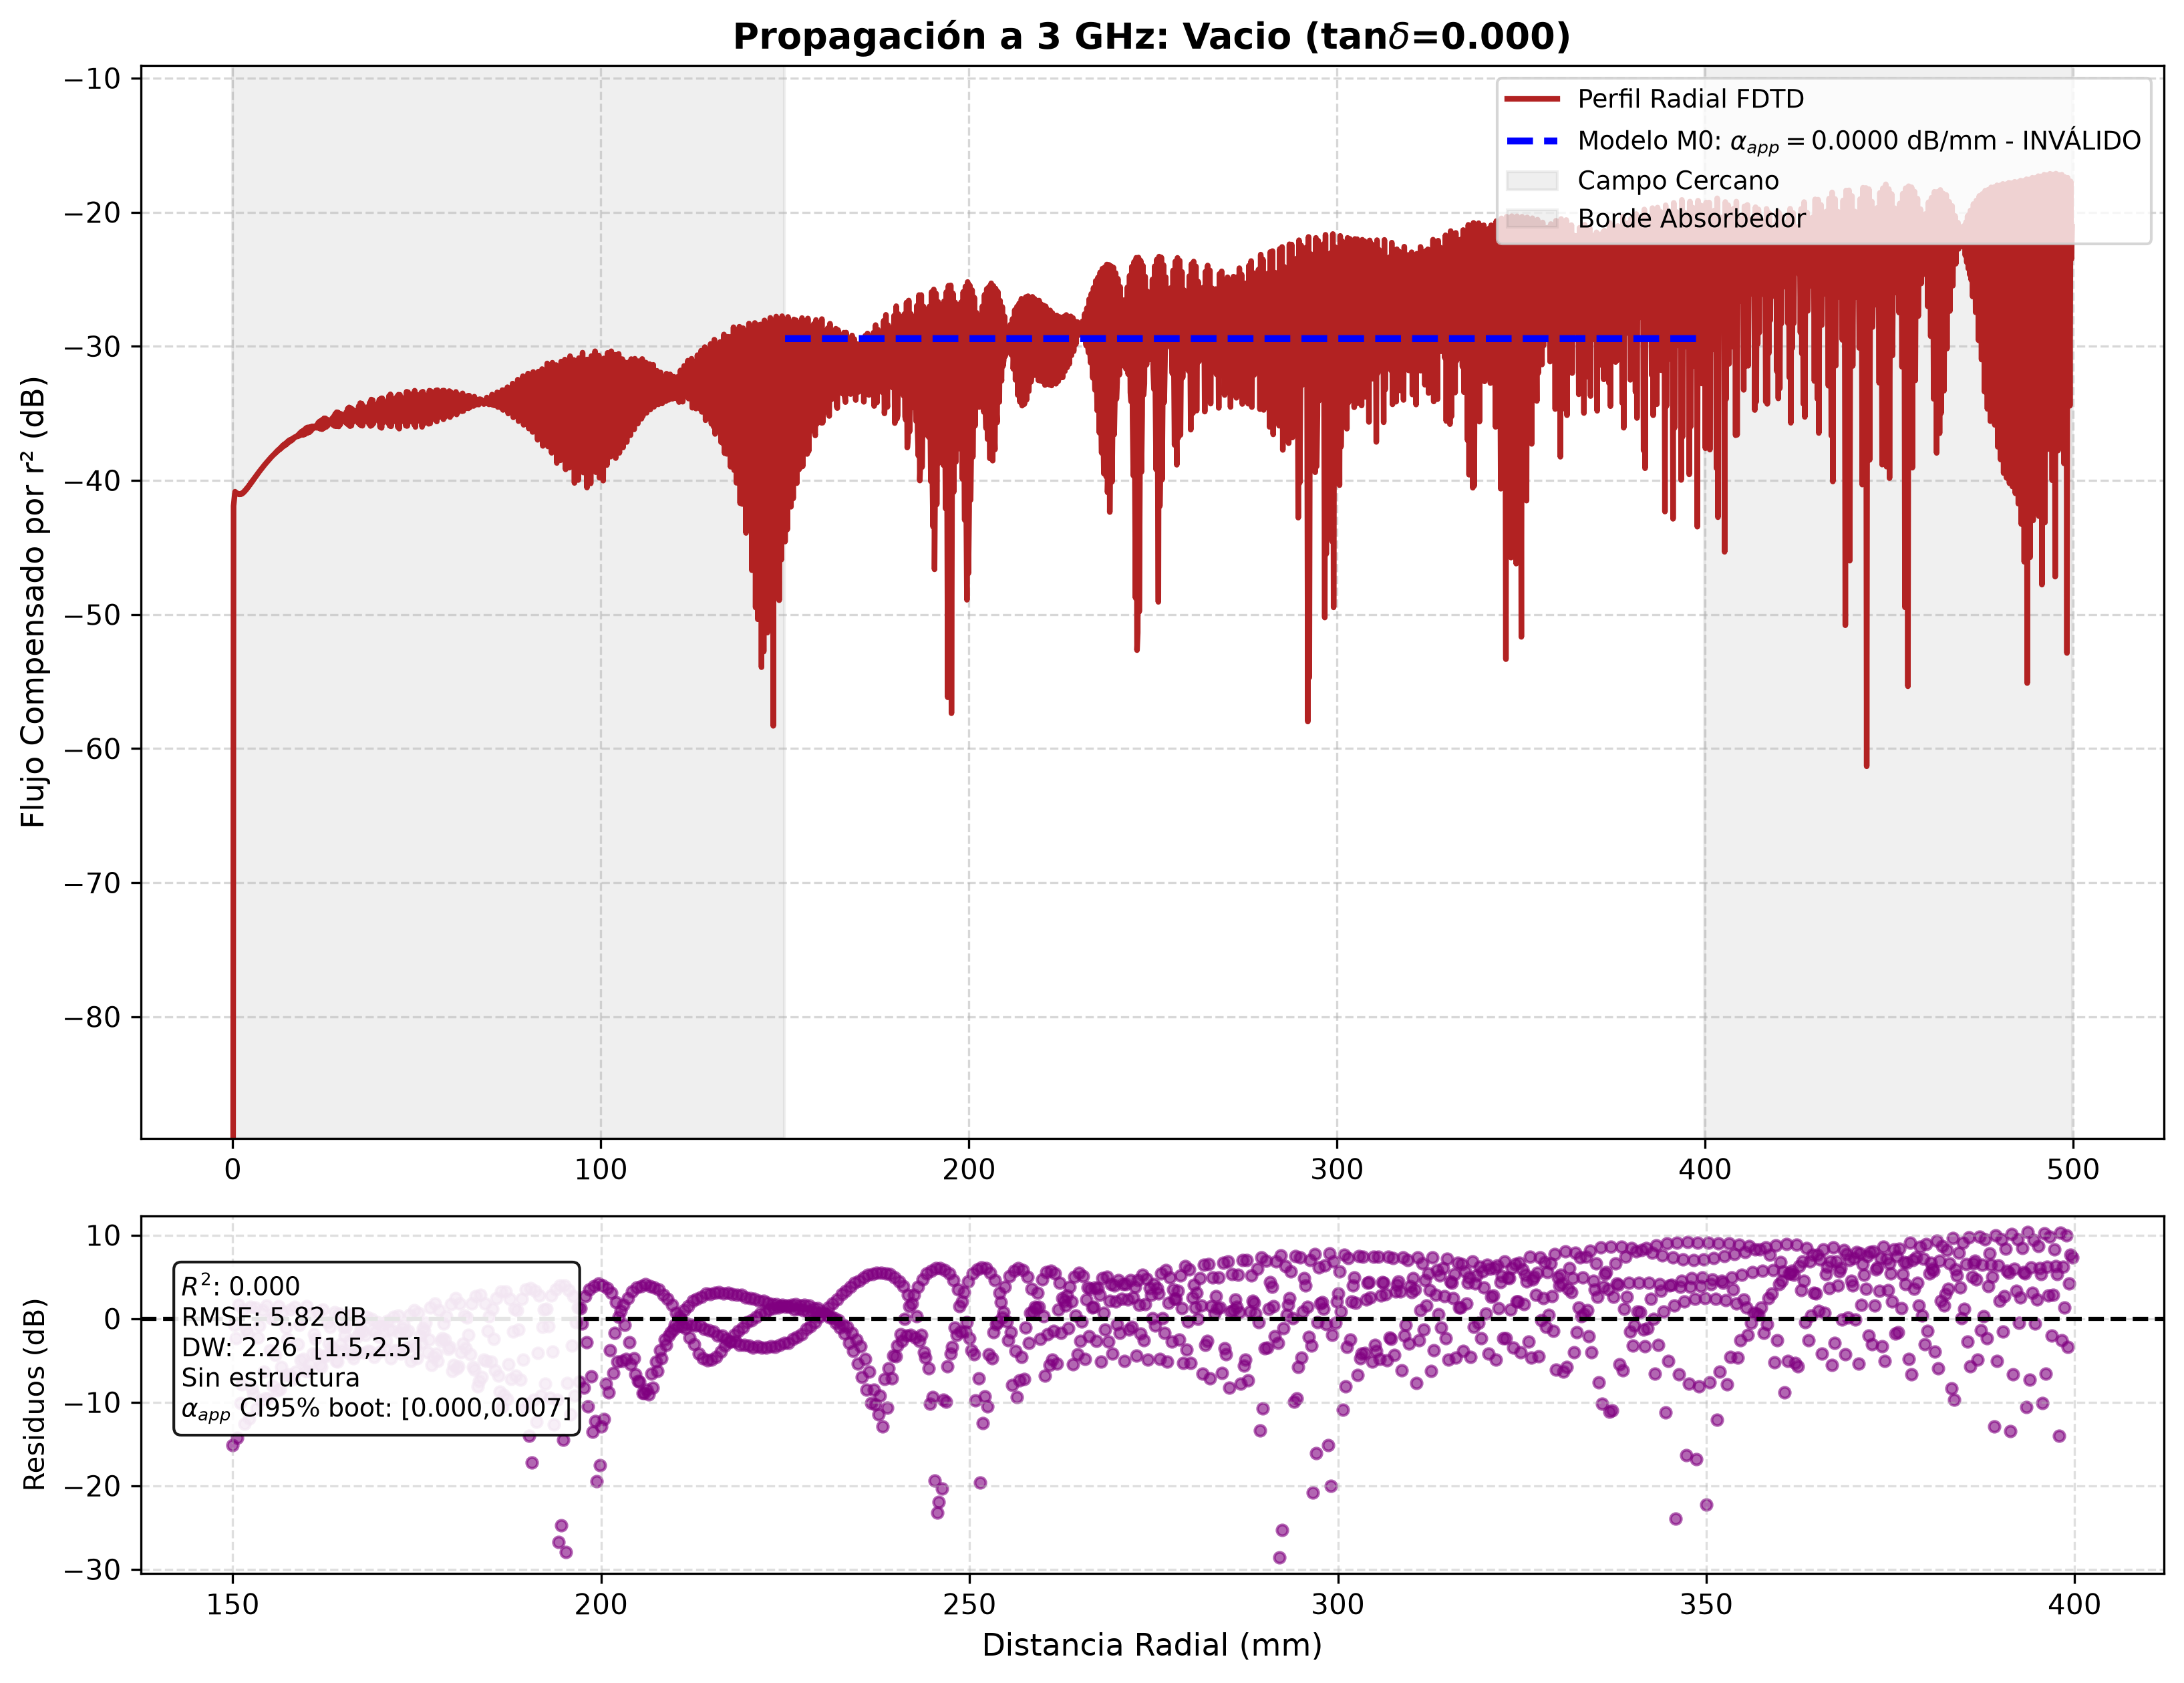
\includegraphics[width=0.81\linewidth]{figuras/Tesis_Resultado_vacio5px.png}\par\smallskip
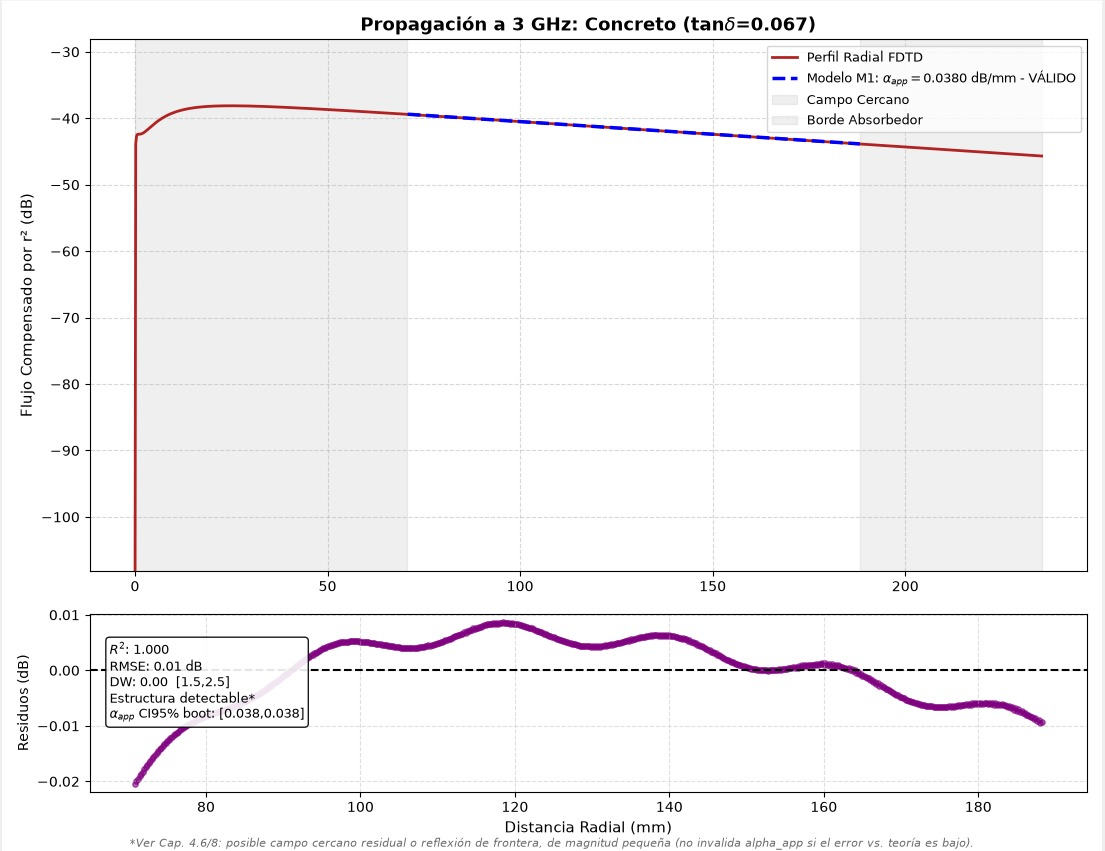
\includegraphics[width=0.81\linewidth]{figuras/Tesis_Resultado_concreto5px.jpeg}
\caption{Perfiles radiales y residuos a 5 px/mm en vacío (arriba) y concreto (abajo). Cada panel conservó su escala vertical.}\label{fig:perfiles-vacio-concreto}\end{figure}

\begin{figure}[htbp]\centering
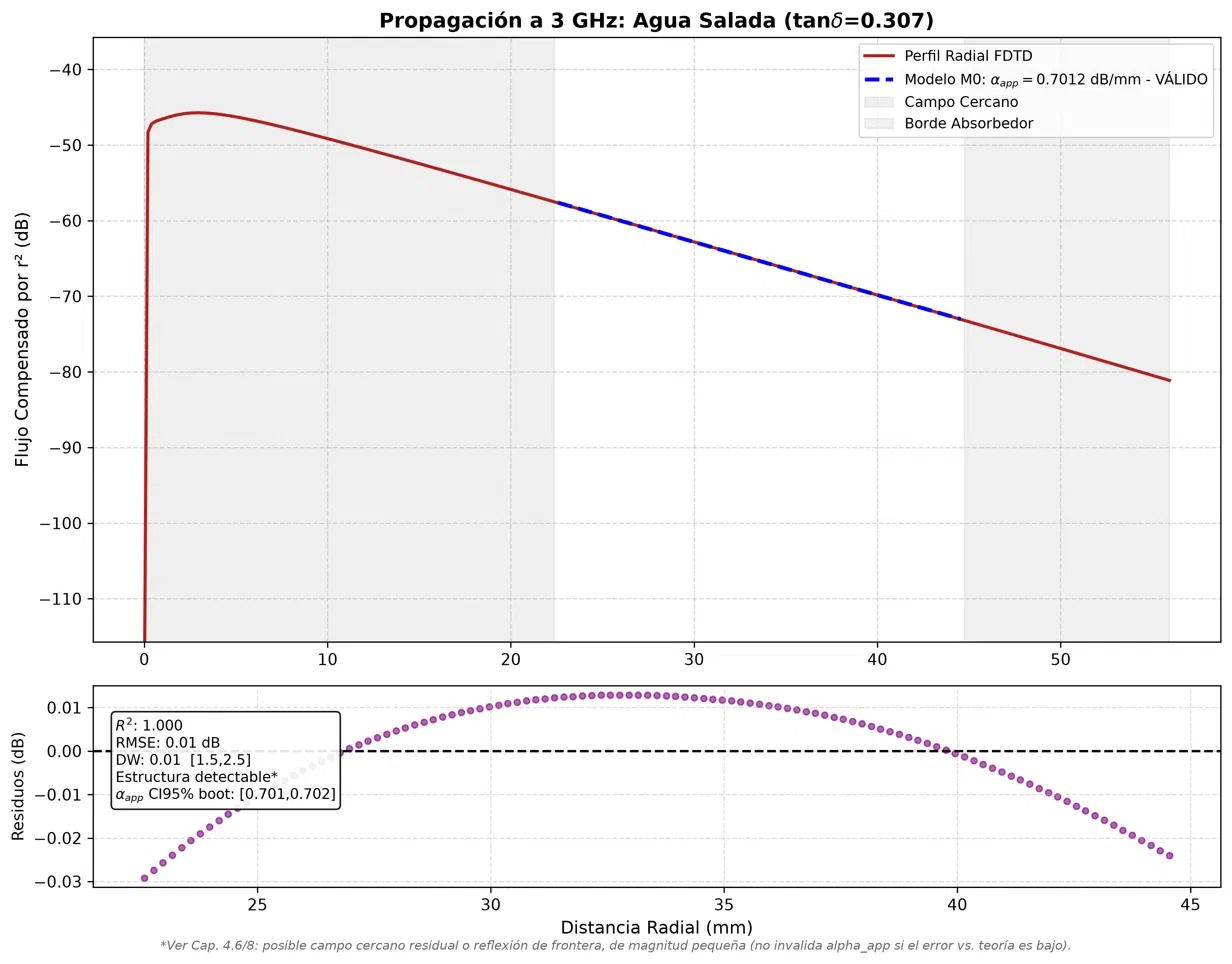
\includegraphics[width=0.81\linewidth]{figuras/Tesis_Resultado_agua_salada5px.jpeg}\par\smallskip
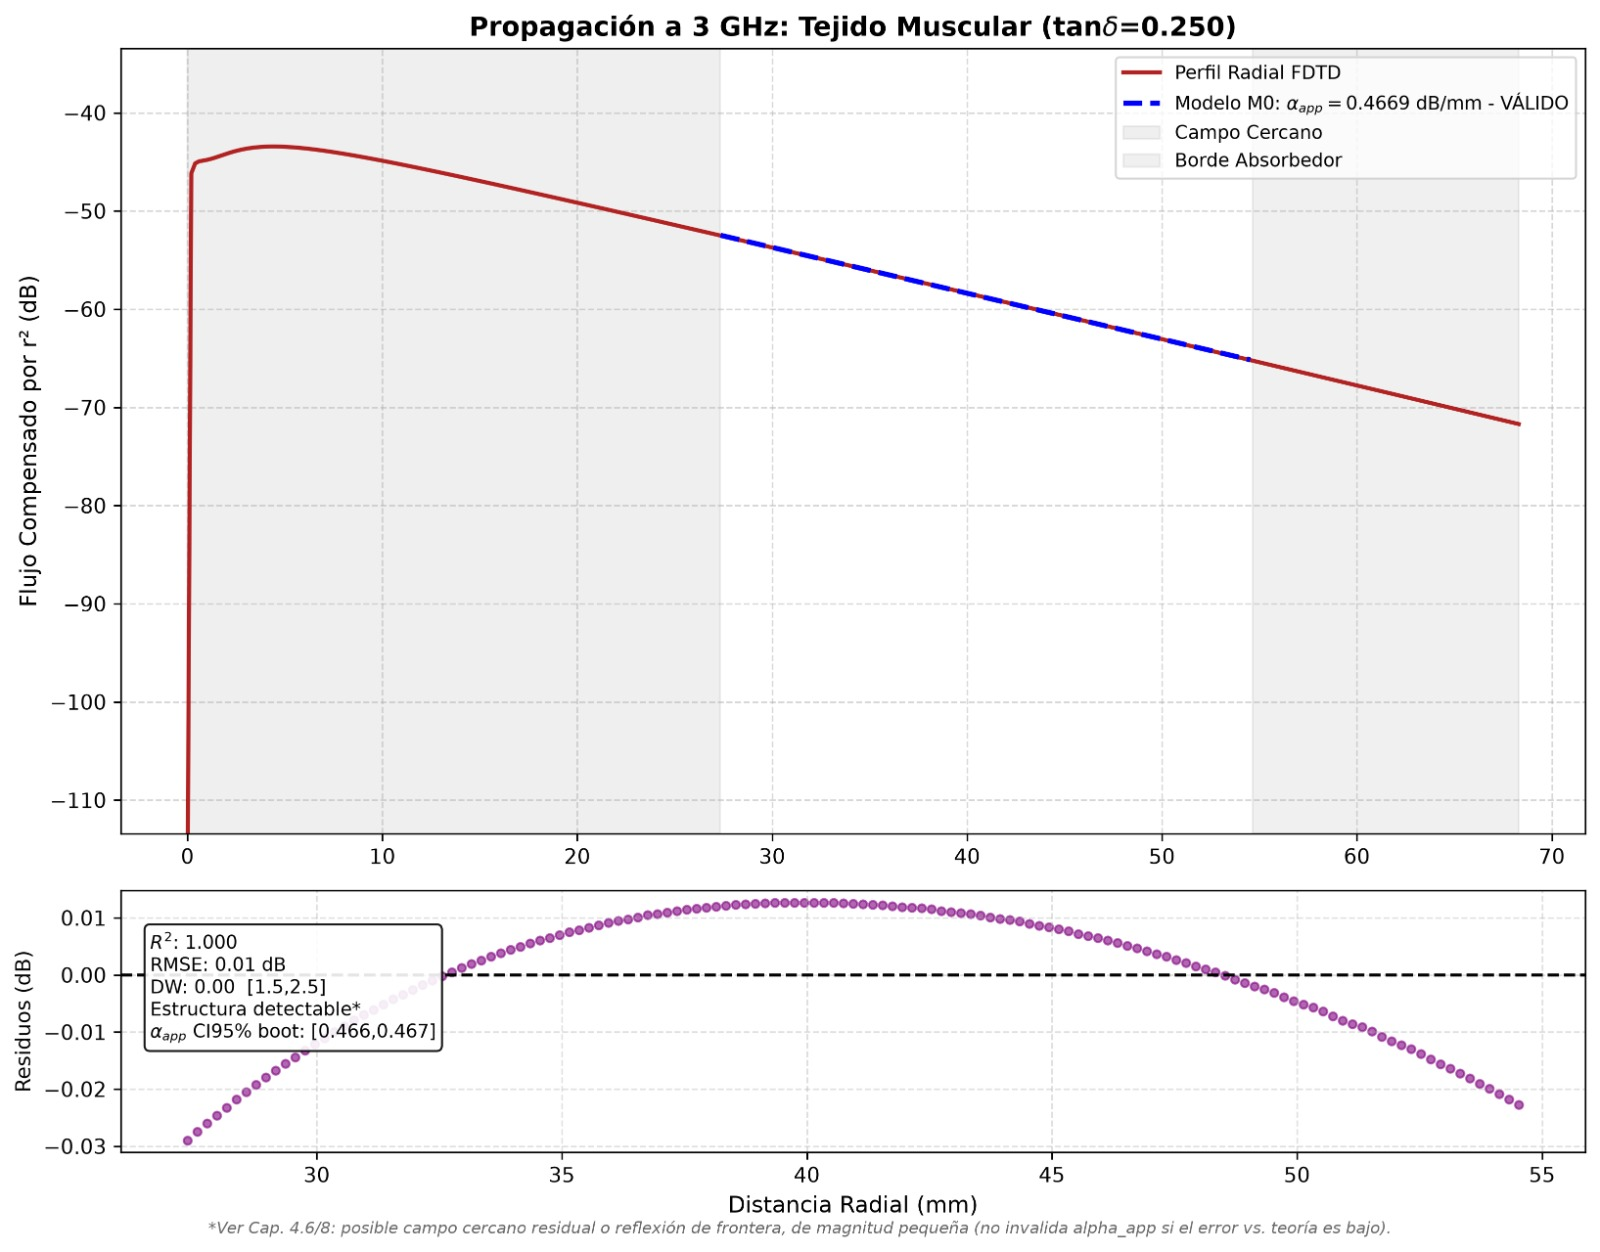
\includegraphics[width=0.81\linewidth]{figuras/Tesis_Resultados_Tejido_Muscular5px.jpeg}
\caption{Perfiles radiales y residuos a 5 px/mm en agua salada (arriba) y tejido muscular (abajo).}\label{fig:perfiles-agua-musculo}\end{figure}

\section{Efecto del refinamiento de malla}
Se examinó la evolución de la pendiente al reducir el paso espacial $h=1/R$, donde $R$ se expresó en px/mm y $h$ en mm. El Cuadro~\ref{tab:fdtd-mallas} reunió las seis corridas adicionales. Los intervalos conservaron la precisión del archivo de origen. En concreto a 10 px/mm ambos extremos coincidieron al redondearse a cuatro decimales.
\begin{table}[htbp]\centering\small\caption{Atenuación e incertidumbre del ajuste en las mallas adicionales.}\label{tab:fdtd-mallas}
\begin{tabular}{lccc}\hline Medio & $R$ (px/mm) & $\alpha_{\mathrm{app}}$ (dB/mm) & IC del 95\,\% (dB/mm) \\ \hline
Agua salada & 10 & 0.7133 & $[0.7130,0.7136]$ \\ & 20 & 0.7224 & $[0.7222,0.7226]$ \\ & 40 & 0.7267 & $[0.7267,0.7268]$ \\
Tejido muscular & 10 & 0.4778 & $[0.4776,0.4780]$ \\ & 20 & 0.4843 & $[0.4842,0.4845]$ \\
Concreto & 10 & 0.0381 & $[0.0381,0.0381]$ \\ \hline\end{tabular}\end{table}

En agua salada, los incrementos sucesivos de la pendiente fueron 0.0121, 0.0091 y 0.0043 dB/mm al duplicarse la resolución. La estimación a 5 px/mm difirió en 3.51\,\% de la obtenida a 40 px/mm. La última estimación quedó a 0.81\,\% del valor teórico. El orden aparente $p=\log_2(|\alpha_{2R}-\alpha_R|/|\alpha_{4R}-\alpha_{2R}|)$ cambió de 0.41 a 1.08 entre los dos tríos de mallas. Además, la selección del modelo pasó de M0 a M1 entre 10 y 20 px/mm. Se observó, por tanto, una aproximación monótona con incrementos decrecientes, aunque la variación del orden y del modelo limitó la interpretación de una extrapolación al continuo. Se reportó la diferencia entre mallas como medida empírica de sensibilidad.

En tejido muscular, el paso de 5 a 10 px/mm elevó la atenuación de 0.4669 a 0.4778 dB/mm. A 20 px/mm se obtuvo 0.4843 dB/mm. La diferencia entre las mallas extremas representó 3.59\,\% del valor más fino. La selección del ajuste también cambió de M0 a M1 en la malla más fina. En concreto, las pendientes a 5 y 10 px/mm difirieron aproximadamente en 0.26\,\% respecto de la segunda, según los valores redondeados. Para el vacío sólo se dispuso de una resolución, por lo que quedó indeterminado el error de discretización.

\subsection{Alcance de la resolución común}
A 5 px/mm se obtuvo un paso de 0.2 mm. Las longitudes de onda registradas correspondieron aproximadamente a 500 celdas en vacío, 235 en concreto, 56 en agua salada y 68 en músculo. En cambio, el diámetro de 0.4 mm del monopolo ocupó apenas dos celdas. La malla común permitió comparar los cuatro medios bajo la misma discretización geométrica. Su alcance quedó cuantificado para la atenuación por las diferencias frente a las mallas más finas disponibles. Estas diferencias fueron específicas de cada medio y también recogieron el efecto de la selección del ajuste.

Las restricciones de hardware limitaron los refinamientos, en particular en los dominios de mayor longitud de onda. Se utilizó una malla cilíndrica axisimétrica en las coordenadas $r$ y $z$, con modo azimutal $m=0$. Para un dominio físico fijo, al duplicarse la resolución se cuadruplicó aproximadamente el número de celdas. A igual factor de Courant y duración física, también se duplicó el número de pasos temporales, de modo que el número total de actualizaciones aumentó aproximadamente por un factor de ocho. Estas relaciones describieron el costo esperado. Los archivos históricos de atenuación carecieron de registros de memoria máxima y tiempo de ejecución por corrida. La campaña adicional de balance incorporó estas mediciones (Cuadro~\ref{tab:balance-costo}).

\section{Identificación de las corridas de balance}
Se utilizó el prefijo B para identificar una corrida de balance. Las letras AS, VA, CO y TM correspondieron a agua salada, vacío, concreto y tejido muscular. Los números 05 y 10 indicaron la resolución en px/mm. Así, B-AS05 designó agua salada a 5 px/mm y B-AS10, agua salada a 10 px/mm. B-VA05, B-CO05 y B-TM05 identificaron los otros tres medios a 5 px/mm. El índice del Anexo~\ref{an:balance-registros} vinculó estas abreviaturas con los archivos completos.

Las potencias tabuladas se expresaron como valores normalizados $P/P_*$, donde $P_*=E_*^2a^2/Z_0$ y $a=1$ mm. La escala de campo $E_*$ quedó pendiente de calibración. Los tiempos de simulación se expresaron en unidades de $a/c=3.33564$ ps. Las conversiones y la conductividad normalizada se definieron en la Sección~\ref{sec:unidades-campana}.

\section{Balance energético local en agua salada a 5 px/mm}\label{sec:balance-agua-cinco}
Se realizó una corrida adicional a 3 GHz para medir el flujo con signo y la disipación de Joule en una misma región. Se seleccionó un volumen anular de agua salada sin fuentes ni metal, comprendido entre $r=\lambda$ y $2\lambda$ y entre $z=0.25\lambda$ y $1.25\lambda$, donde $\lambda=11.187$ mm. Se sincronizaron los campos eléctrico y magnético y se integró el flujo con el factor de superficie cilíndrico correspondiente a cada cara. La potencia disipada se obtuvo independientemente mediante la integración volumétrica de la densidad de pérdida óhmica.

\begin{table}[htbp]\centering\small
\caption{Potencias del balance en el anillo de agua salada, normalizadas por $P_*$. Las muestras correspondieron a $t_1=1740.3$ y $t_2=1840.3$ en unidades temporales de Meep. Se indicaron magnitudes y sentido del flujo por separado.}\label{tab:balance-agua-cinco}
\begin{tabular}{lrr}\hline
Término & Primera muestra & Segunda muestra \\ \hline
Pared interior (entrada) & $1.239894\times10^{-5}$ & $1.239894\times10^{-5}$ \\
Tapa inferior (entrada) & $2.918001\times10^{-6}$ & $2.918001\times10^{-6}$ \\
Pared exterior (salida) & $2.000278\times10^{-6}$ & $2.000280\times10^{-6}$ \\
Tapa superior (salida) & $8.755799\times10^{-7}$ & $8.755806\times10^{-7}$ \\
Disipación de Joule & $1.243268\times10^{-5}$ & $1.243268\times10^{-5}$ \\
Residuo & $8.396156\times10^{-9}$ & $8.392715\times10^{-9}$ \\ \hline
\end{tabular}\end{table}

Se sumaron los flujos netos de las dos caras de entrada para obtener $P_{\rm ent}$ y los de las dos caras de salida para obtener $P_{\rm sal}$. El residuo se calculó mediante $R=P_{\rm ent}-P_{\rm sal}-P_{\rm J}$. En la segunda muestra, la disipación representó el 81.1695\,\% de $P_{\rm ent}$ y el flujo saliente, el 18.7757\,\%. El residuo relativo $100R/P_{\rm ent}$ pasó de 0.054816\,\% a 0.054794\,\% entre ambas muestras. Al normalizarlo exclusivamente por la entrada de la pared interior, tal como se registró en el archivo de la corrida, se obtuvo 0.067689\,\% en la segunda muestra.

Durante el intervalo de aproximadamente un período, el mayor cambio relativo entre las cuatro potencias de cara y la disipación fue de 0.000107\,\% respecto de la primera muestra del mismo término. Se registraron 157.3 s de ejecución y un máximo de 178.6 MiB de memoria residente del proceso en Ubuntu bajo WSL, con un procesador AMD Ryzen 5 4600H y un hilo de cómputo. Estas mediciones correspondieron a la corrida B-AS05. Posteriormente se completaron los balances B-VA05, B-CO05 y B-TM05 para los otros tres medios y B-AS10 para agua salada a 10 px/mm.

\section{Comparación del balance en los cuatro medios}\label{sec:balance-comparativo}
Se completó la misma medición anular en cada medio a 5 px/mm. Se conservaron los límites $r\in[\lambda,2\lambda]$ y $z\in[0.25\lambda,1.25\lambda]$, de modo que el volumen físico cambió con la longitud de onda. Se calculó la densidad media de flujo mediante $S_r=-\operatorname{Re}(E_zH_\phi^*)/2$ y $S_z=\operatorname{Re}(E_rH_\phi^*)/2$. La pérdida se integró como
\begin{equation}
 P_{\rm J}=\int_{\lambda}^{2\lambda}\int_{0.25\lambda}^{1.25\lambda}
 \frac{\varepsilon_r\sigma_D}{2}\left(|E_r|^2+|E_z|^2\right)2\pi r\, dz\,dr,
 \label{eq:joule-anular}
\end{equation}
donde $\sigma_D$ correspondió a la conductividad del término de evolución de $D$ en unidades de Meep. Se empleó cuadratura trapezoidal con paso de muestreo igual o inferior a una celda. El factor $2\pi r$ se incorporó explícitamente tanto en el volumen como en las superficies correspondientes.

Se orientaron hacia fuera las normales de las cuatro caras y se denotaron sus flujos netos por $F_j$. Con esta convención se obtuvieron
\begin{equation}
 P_{\rm ent}=-\sum_j\min(F_j,0),\qquad
 P_{\rm sal}=\sum_j\max(F_j,0),\qquad
 \eta_{\rm J}=\frac{P_{\rm J}}{P_{\rm ent}},\qquad
 \delta_{\rm B}=\frac{P_{\rm ent}-P_{\rm sal}-P_{\rm J}}{P_{\rm ent}}.
 \label{eq:balance-normalizado}
\end{equation}
La agrupación por signo se efectuó sobre el flujo integrado de cada cara. Las potencias se expresaron en unidades de Meep y las fracciones se normalizaron por la entrada neta total al anillo. El Cuadro~\ref{tab:balance-medios} presentó la segunda muestra de cada corrida. Los identificadores remitieron a los archivos individuales del \hyperref[an:balance-registros]{Anexo A}.

\begin{table}[htbp]\centering\small
\caption{Balance local a 5 px/mm. Las tres últimas columnas se expresaron como porcentajes de $P_{\rm ent}$ y su suma fue 100, dentro del redondeo. El residuo conservó su signo.}\label{tab:balance-medios}
\begin{tabular}{llrrrr}\hline
Medio & ID & $P_{\rm ent}/P_*$ & Disipada & Saliente & Residuo \\ \hline
Vacío & B-VA05 & $1.094598\!\times\!10^{-3}$ & 0.0000 & 99.9861 & 0.013943 \\
Concreto & B-CO05 & $3.686265\!\times\!10^{-4}$ & 30.3782 & 69.6198 & 0.002011 \\
Agua salada & B-AS05 & $1.531694\!\times\!10^{-5}$ & 81.1695 & 18.7757 & 0.054794 \\
Músculo & B-TM05 & $3.819407\!\times\!10^{-5}$ & 74.5328 & 25.4343 & 0.032973 \\ \hline
\end{tabular}\end{table}

En los cuatro medios, la pared interior y la tapa inferior aportaron potencia al anillo, mientras que la pared exterior y la tapa superior registraron salida. Se obtuvo la mayor fracción disipada en agua salada, seguida del músculo y del concreto. En vacío, $P_{\rm J}=0$ se siguió directamente de la conductividad nula asignada. La entrada y la salida concordaron dentro del residuo informado. Las potencias absolutas correspondieron a la amplitud numérica de excitación utilizada y su conversión a vatios quedó condicionada a una calibración de la fuente.

\subsection{Variación entre las dos muestras temporales}
Se registraron dos muestras separadas aproximadamente por un período de la fuente, después del tiempo de estabilización del simulador. Para comparar los medios con una normalización común se definió
\begin{equation}
 \Delta_{\rm t}=\frac{\max_k|Q_k(t_2)-Q_k(t_1)|}{P_{\rm ent}(t_2)},
 \label{eq:variacion-temporal}
\end{equation}
donde $Q_k$ recorrió las cuatro potencias de cara y $P_{\rm J}$. Se incluyeron por separado ambos residuos en el Cuadro~\ref{tab:balance-tiempo}.

\begin{table}[htbp]\centering\small
\caption{Comprobación temporal del balance. Los tiempos se expresaron en unidades de Meep y las tres últimas columnas en porcentaje. $\delta_{\rm B}$ se normalizó por la entrada de su propia muestra.}\label{tab:balance-tiempo}
\begin{tabular}{lrrrrr}\hline
ID & $t_1$ & $t_2$ & $100\delta_{\rm B}(t_1)$ & $100\delta_{\rm B}(t_2)$ & $100\Delta_{\rm t}$ \\ \hline
B-VA05 & 3497.60 & 3597.60 & 0.000308 & 0.013943 & 0.017448 \\
B-CO05 & 3496.80 & 3596.80 & 0.001772 & 0.002011 & 0.000143 \\
B-AS05 & 1740.30 & 1840.30 & 0.054816 & 0.054794 & 0.000014 \\
B-TM05 & 1743.10 & 1843.10 & 0.032984 & 0.032973 & 0.000005 \\
B-AS10 & 1740.30 & 1840.25 & 0.021675 & 0.021640 & 0.000021 \\ \hline
\end{tabular}\end{table}

Los términos variaron menos de 0.000144\,\% de la entrada final en los medios con pérdidas. En vacío se observó una variación mayor, de 0.017448\,\%, y el residuo aumentó durante el último intervalo. La comprobación quedó limitada a dos instantes de fase aproximadamente equivalente. La ausencia de una serie temporal extensa dejó sin cuantificar el almacenamiento residual de energía y la estabilidad a tiempos mayores.

\subsection{Sensibilidad del balance de agua salada al refinamiento}
Se repitió la integración en el mismo anillo físico a 10 px/mm. Se obtuvo $P_{\rm ent}=1.073782\times10^{-5}$ y $P_{\rm J}=8.679552\times10^{-6}$ en unidades de Meep. La fracción disipada pasó de 81.1695\,\% a 80.8316\,\%, la fracción saliente alcanzó 19.1468\,\% y el residuo descendió a 0.021640\,\%. La reducción de la fracción disipada fue de 0.337943 puntos porcentuales, equivalente al 0.418083\,\% de la fracción obtenida con la malla fina.

La entrada absoluta disminuyó 29.8958\,\% y la disipación absoluta, 30.1876\,\%, respecto de la malla de 5 px/mm. La normalización compensó gran parte de esta variación común. Por ello, la sensibilidad de 0.4181\,\% caracterizó específicamente el cociente $\eta_{\rm J}$. Dos resoluciones proporcionaron una diferencia observada entre mallas, mientras que la estimación del orden de convergencia del balance y de su error al continuo quedó pendiente. Para concreto, músculo y vacío se contó con una sola malla de balance.

Los resultados de balance se acompañaron de sus residuos, variaciones temporales y, en agua salada, de la diferencia entre mallas. Estos diagnósticos describieron fuentes distintas de discrepancia numérica. La disponibilidad de dos muestras deterministas dejó sin estimar una incertidumbre estadística del balance. Los IC del ajuste de atenuación se mantuvieron asociados exclusivamente a aquella extracción.

\clearpage
\subsection{Costo computacional medido}\label{sec:costo-balance}
Las cuatro corridas adicionales se ejecutaron secuencialmente mediante tareas de VS Code conectado a Ubuntu bajo WSL2. Se utilizó un procesador AMD Ryzen 5 4600H, con un hilo OpenMP y uno OpenBLAS por proceso. El entorno dispuso de 7.44 GiB de memoria total. Se emplearon Python 3.13.13, NumPy 2.4.3 y Meep 1.33.0-beta. El Cuadro~\ref{tab:balance-costo} incluyó también la corrida B-AS05 previamente completada.

\begin{table}[htbp]\centering\small
\caption{Tiempo de pared y memoria residente máxima de cada proceso de balance. El tiempo incluyó inicialización, avance temporal, extracción e integración.}\label{tab:balance-costo}
\begin{tabular}{lrrr}\hline
ID & Resolución (px/mm) & Tiempo (s) & RSS máxima (MiB) \\ \hline
B-VA05 & 5 & 26977.1 & 4868.2 \\
B-CO05 & 5 & 6491.7 & 1326.1 \\
B-AS05 & 5 & 157.3 & 178.6 \\
B-TM05 & 5 & 300.3 & 213.2 \\
B-AS10 & 10 & 1581.1 & 384.3 \\ \hline
\end{tabular}\end{table}

El vacío requirió 7.49 h y 4.75 GiB de RSS máxima, mientras que el concreto requirió 1.80 h. En agua salada, duplicar la resolución elevó el tiempo por un factor de 10.05 y la RSS por un factor de 2.15. Estos cocientes describieron las ejecuciones medidas y dependieron también de los costos fijos y de la actividad del sistema. El escalado cuadrático ideal de memoria aplicado al vacío a 10 px/mm habría supuesto aproximadamente 19 GiB, por encima de la memoria disponible en WSL. Esta proyección se distinguió del consumo efectivamente medido y sustentó la restricción práctica de la comparación común a 5 px/mm.


\section{Verificación de propagación uniforme}\label{sec:resultados-planar}
La campaña VP comprendió ocho corridas independientes de la antena. En los medios disipativos, los errores de atenuación respecto de la solución analítica fueron inferiores a 0.16\,\% a 5 px/mm y a 0.041\,\% a 10 px/mm (Cuadro~\ref{tab:planar}). En vacío se obtuvieron pendientes de $-2.80\times10^{-11}$ y $2.01\times10^{-10}$ dB/mm, compatibles con cero dentro de sus IC. Al ser nula la referencia, se informó la diferencia absoluta y se omitió el error relativo.

\begin{table}[htbp]\centering\footnotesize
\caption{Verificación planar: atenuación e IC condicional del 95\,\% en dB/mm. El error relativo se calculó respecto de la solución analítica. Las cifras adicionales permitieron distinguir el IC del error sistemático.}\label{tab:planar}
\begin{tabular}{lrrr}\hline
ID & $\alpha_{\rm VP}$ & IC del ajuste & Error (\%) \\ \hline
VP-VA05 & $-2.80\times10^{-11}$ & $[-6.61\times10^{-8},\,6.53\times10^{-8}]$ & --- \\
VP-VA10 & $2.01\times10^{-10}$ & $[-2.01\times10^{-8},\,2.14\times10^{-8}]$ & --- \\
VP-CO05 & $0.038546428$ & $[0.038546315,\,0.038546532]$ & 0.0095 \\
VP-CO10 & $0.038543997$ & $[0.038543964,\,0.038544028]$ & 0.0032 \\
VP-AS05 & $0.733774319$ & $[0.733756741,\,0.733792172]$ & 0.1575 \\
VP-AS10 & $0.732914311$ & $[0.732911332,\,0.732917661]$ & 0.0401 \\
VP-TM05 & $0.492580649$ & $[0.492576832,\,0.492584230]$ & 0.1060 \\
VP-TM10 & $0.492193312$ & $[0.492191869,\,0.492194743]$ & 0.0273 \\
\hline\end{tabular}\end{table}

La variación temporal máxima del flujo fue inferior a $7.87\times10^{-6}$ en vacío y a $2.95\times10^{-10}$ en los medios disipativos. Los RMSE fueron menores que $1.4\times10^{-5}$ dB en vacío. La Figura~\ref{fig:planar} mostró las diferencias espaciales respecto del perfil analítico, normalizado en el primer punto; las oscilaciones y la deriva restante disminuyeron al refinar la malla en los medios con pérdidas.

\begin{figure}[!htbp]\centering
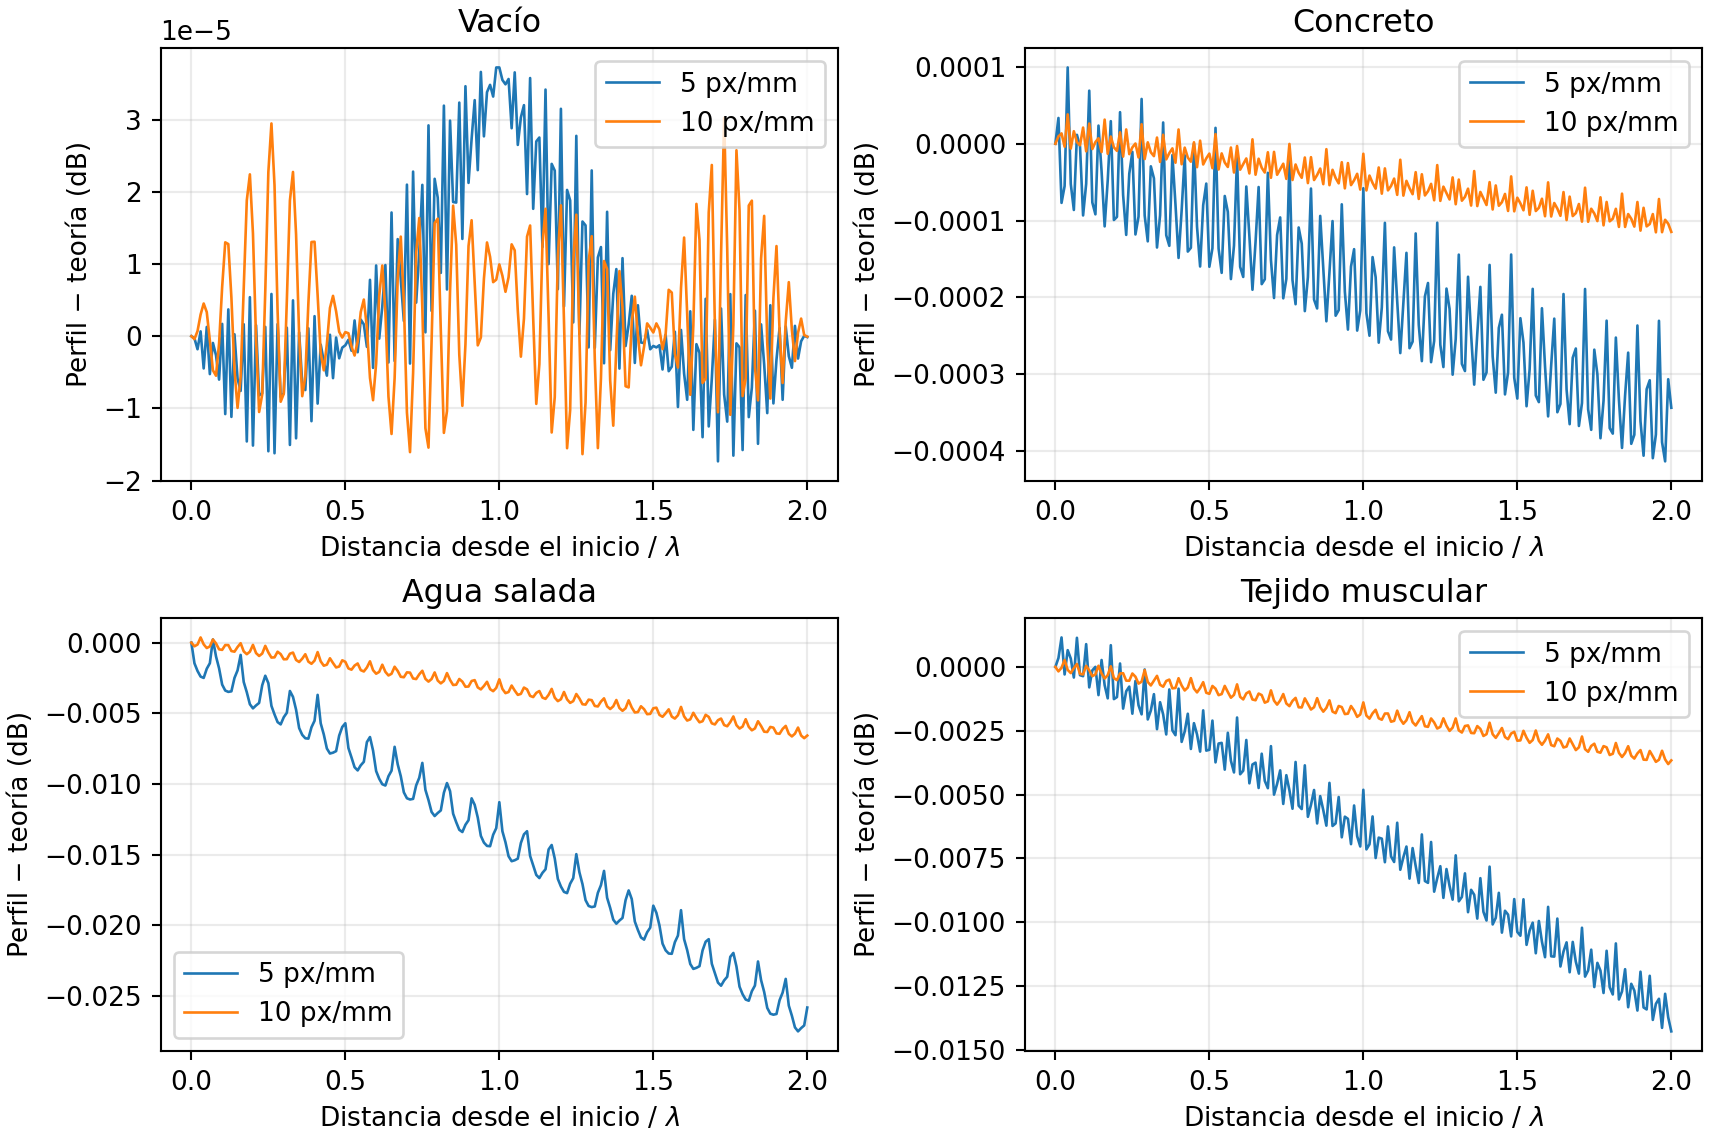
\includegraphics[width=\textwidth]{figuras/verificacion_onda_plana.png}
\caption{Diferencia entre el perfil planar normalizado y la predicción analítica. Cada panel utilizó su propia escala vertical. Se compararon las dos mallas sobre la misma ventana física de cada medio.}\label{fig:planar}
\end{figure}

Una ejecución inicial con encendido abrupto produjo, en vacío a 5 px/mm, un RMSE de 1.13 dB y un cambio temporal del flujo de 0.679. Se descartó como comprobación estacionaria y se conservó como diagnóstico. El cambio de activación redujo ambas discrepancias en esta prueba; los registros originales de la antena permanecieron separados. Se archivaron las dieciséis ejecuciones, sus perfiles y las dos versiones del verificador.

Las ocho corridas con activación suave acumularon 17.9 s de tiempo medido y una RSS máxima del proceso de 111.2 MiB. Se ejecutaron secuencialmente desde VS Code en Ubuntu con un solo hilo. La RSS fue acumulativa dentro del proceso; no se interpretó como el consumo independiente de cada caso.

    \fi  
\fi

% DISCUSION DE RESULTADOS
% --------------------------------------------------------------------------------
\ifdefined\CAPdiscusion
	\newpage
	\chapter{Discusión y análisis de resultados}
	\ifdefined\parpordefecto
    	\defaultparformat{discusion}
    \else
    	\section{Atenuación aparente y comparación con la teoría}
A 3 GHz, el flujo radial compensado decayó más rápidamente en agua salada que en tejido muscular y en concreto. Este orden coincidió con el previsto a partir de la permitividad y la conductividad asignadas a los medios (Cuadro~\ref{tab:fdtd-base}). La compensación por $r^2$ permitió examinar el decaimiento que persistió después de descontar la expansión geométrica esperada en la región de radiación. Sin embargo, la pendiente se estimó sobre una línea de observación y en un intervalo finito de distancias. Por ello se interpretó como una atenuación aparente de la radiación del monopolo y se tomó la atenuación teórica del medio homogéneo como referencia de propagación.

En los tres medios con pérdidas, la simulación subestimó la atenuación teórica. El concreto presentó la menor discrepancia relativa (1.31\,\%), mientras que en agua salada y músculo se obtuvieron diferencias de 4.29\,\% y 5.12\,\%, respectivamente. El orden de estas discrepancias difirió del orden de pérdidas de los materiales. Además, la longitud del monopolo y las dimensiones del dominio se escalaron con la longitud de onda de cada medio. La comparación describió, por tanto, configuraciones eléctricamente semejantes, con distinta longitud física y con un diámetro de conductor fijo. Atribuir las diferencias únicamente a la conductividad habría excedido el alcance de este diseño.

\section{Precisión del ajuste y sensibilidad a la ventana radial}
En tejido muscular a 5 px/mm, el IC del 95\,\% abarcó de 0.4663 a 0.4674 dB/mm, mientras que la separación entre la estimación central y la referencia alcanzó 0.0252 dB/mm. La estrechez del intervalo indicó que se recuperó una pendiente semejante al remuestrear bloques de residuos dentro de la ventana elegida. La discrepancia con la teoría incorporó además la influencia del perfil físico, de su discretización y del modelo empleado para extraer la pendiente. Los valores de Durbin--Watson próximos a cero y la curvatura visible de los residuos señalaron que los puntos radiales contiguos compartieron desviaciones del mismo signo. Esta estructura limitó la interpretación de la precisión estadística como medida de exactitud física.

El barrido del límite inferior permitió examinar esa distinción sin repetir la simulación. En músculo a 5 px/mm, al desplazar el inicio de la ventana de $1.5\lambda$ a $3\lambda$, la estimación con el modelo lineal M0 pasó de 0.4650 a 0.4695 dB/mm. La variación de 0.0045 dB/mm superó la anchura del intervalo obtenido en la ventana principal, y aun el mayor valor permaneció por debajo de la referencia de 0.4921 dB/mm. Así, la ventana explicó parte de la variación de la pendiente. El barrido por sí solo dejó abierta la contribución relativa del campo cercano y de las reflexiones de frontera.

\section{Alcance del refinamiento y del control en vacío}
En agua salada, al pasar de 5 a 40 px/mm, la discrepancia respecto de la teoría descendió de 4.29\,\% a 0.81\,\%. El sentido del cambio y la reducción de los incrementos sucesivos indicaron que el refinamiento mejoró la concordancia. Sin embargo, entre 10 y 20 px/mm la selección pasó de M0 a M1, que incorporó un término sinusoidal. Por ello, la diferencia de 3.51\,\% entre las pendientes de las mallas extremas caracterizó la sensibilidad del procedimiento completo. La variación del orden aparente entre tríos de mallas limitó la extrapolación a paso espacial nulo (Cuadro~\ref{tab:fdtd-mallas}). Los perfiles adicionales se reunieron en el \hyperref[an:fdtd-perfiles]{Anexo B}.

A 5 px/mm, incluso la longitud de onda más corta, la del agua salada, abarcó unas 56 celdas. En cambio, el diámetro del monopolo ocupó sólo dos en todos los medios. Esta diferencia permitió distinguir la resolución de la onda propagada de la representación del conductor. La malla común resultó útil para comparar el orden de atenuación y cuantificar cuánto cambió cada pendiente al refinarla. Las diferencias observadas en concreto y músculo, de aproximadamente 0.26\,\% y 3.59\,\% frente a sus respectivas mallas más finas, delimitaron esa comparación para cada material.

En vacío, la ausencia de pérdidas proporcionó un control particularmente exigente. La estimación alcanzó el límite inferior permitido por el ajuste, con $R^2=0.0000$ y un RMSE de 5.8227 dB. El perfil compensado presentó oscilaciones intensas y la coincidencia numérica con la atenuación teórica nula tuvo escaso valor probatorio. Con una sola malla quedó abierta la distinción entre efectos de frontera y de discretización. Por último, el análisis radial cuantificó el decaimiento espacial del flujo observado. Para establecer qué fracción de la potencia se disipó en el medio se requirió una comprobación independiente del balance sobre un volumen de control.

\section{Interpretación del balance local en agua salada}
La tapa inferior aportó potencia al volumen de control (Cuadro~\ref{tab:balance-agua-cinco}). Si sólo se hubiera contado la entrada radial, la disipación habría representado el 100.27\,\% de esa entrada. Al incorporar el transporte axial a través de la tapa inferior, la fracción disipada fue del 81.17\,\% de la entrada total. Así se explicó, mediante las direcciones de flujo medidas, por qué el perfil radial de atenuación resultó insuficiente para reconstruir la pérdida integrada en el anillo.

El residuo del 0.0548\,\% y la escasa variación de los términos durante el último período respaldaron el cierre local del balance para esta geometría y esta malla. La fracción disipada caracterizó la energía que atravesó el anillo seleccionado y dependió de sus límites. El residuo cuantificó la discrepancia de cierre entre integrales calculadas en la misma corrida. La repetición a 10 px/mm redujo la fracción disipada en 0.337943 puntos porcentuales. La diferencia relativa de 0.4181\,\% respecto de la malla fina fue pequeña frente al cambio cercano al 30\,\% de las potencias absolutas. Este contraste mostró que la normalización absorbió buena parte de la dependencia de la amplitud con la malla. La representación de un conductor de dos celdas de diámetro y de una fuente de dimensiones reducidas ofreció una explicación plausible de esa sensibilidad, cuya contribución individual quedó sin aislar.

\section{Conservación local y alcance de la validación física}
La disipación integrada conservó el orden observado en la atenuación de los medios con pérdidas. Las fracciones de 81.17\,\%, 74.53\,\% y 30.38\,\% en agua salada, músculo y concreto describieron el destino de la potencia que entró en cada anillo (Cuadro~\ref{tab:balance-medios}). Los límites se expresaron en longitudes de onda y correspondieron a volúmenes físicos diferentes. La comparación quedó, por ello, referida a regiones eléctricamente semejantes. La interpretación como eficiencia total de radiación o como fracción de la potencia suministrada por el generador quedó fuera del alcance de estas superficies de control.

En vacío, la conductividad nula impuso la ausencia de pérdida de Joule. La comprobación adicional consistió en contrastar de forma independiente los flujos entrantes y salientes. El residuo final de 0.013943\,\% mostró una concordancia estrecha entre ambos, aunque aumentó desde 0.000308\,\% durante el último intervalo. La máxima variación temporal de un término fue de 0.017448\,\% de la entrada final, comparable en magnitud con ese residuo. En consecuencia, la comprobación temporal exigió mayor cautela en vacío. La conservación local aportó un control físico complementario al ajuste radial, cuyo criterio de calidad había fallado.

En concreto, agua salada y músculo, los residuos finales de 0.002011\,\%, 0.054794\,\% y 0.032973\,\% se acompañaron de cambios temporales de los términos inferiores a 0.000144\,\% de la entrada. Esta separación de magnitudes respaldó la estabilidad de las integrales en los dos instantes examinados. En agua salada, el descenso del residuo al refinar la malla también resultó compatible con una contribución de la discretización y de la cuadratura. El almacenamiento transitorio de energía, la interpolación de campos y las integrales de superficie y volumen pudieron contribuir simultáneamente al cierre observado. La disponibilidad de dos muestras, tomadas a una separación cercana a un período, limitó la evaluación de transitorios más lentos.

\section{Incertidumbres y alcance de la resolución adoptada}
Se distinguieron tres niveles de evaluación. El remuestreo por bloques cuantificó la incertidumbre condicional del ajuste de atenuación. La comparación con la solución analítica del medio homogéneo midió la discrepancia física de la pendiente aparente. Las diferencias entre mallas describieron la sensibilidad del procedimiento numérico completo, incluidos el muestreo y la selección del modelo de ajuste. La ausencia de un orden asintótico estable dejó sin determinar una cota del error de discretización al continuo. Para el balance se añadieron los diagnósticos de cierre y de variación temporal, y quedó pendiente una estimación global de incertidumbre que integrara esas contribuciones.

La resolución común de 5 px/mm se sustentó en una precisión y un costo explícitos. Permitió recuperar el orden de atenuación de los medios con pérdidas, con discrepancias teóricas entre 1.31\,\% y 5.12\,\%, y diferencias frente a las mallas más finas disponibles de 0.26\,\% a 3.59\,\%. En el balance de agua salada, el refinamiento a 10 px/mm modificó la fracción disipada en 0.42\,\% respecto del valor fino. A la vez, la dependencia de las potencias absolutas y la representación limitada del conductor restringieron la precisión atribuible a la malla común.

El costo medido reforzó esa delimitación. El vacío consumió 4.75 GiB de memoria residente y 7.49 h a 5 px/mm, dentro de un entorno WSL con 7.44 GiB de memoria total (Cuadro~\ref{tab:balance-costo}). Un refinamiento sistemático de todos los medios habría requerido recursos adicionales. Así, la comparación a 5 px/mm se justificó para las tendencias y los cocientes documentados, con los márgenes observados en cada magnitud. La validación alcanzada combinó concordancia teórica de la atenuación en los medios con pérdidas, sensibilidad de malla y cierre energético local. Su extensión a potencias absolutas convergidas, a la eficiencia global de la antena y a otros parámetros materiales quedó pendiente de verificaciones específicas.

\section{Pérdidas de propagación y evaluación de los objetivos}
Los perfiles de las Figuras~\ref{fig:perfiles-vacio-concreto} y~\ref{fig:perfiles-agua-musculo} permitieron examinar el decaimiento y la estructura de los residuos en la malla común. Las seis figuras del Anexo~\ref{an:fdtd-perfiles} respaldaron las comparaciones de refinamiento. En agua salada se observó una aproximación progresiva a la pendiente teórica. En músculo y concreto se cuantificó la sensibilidad con las resoluciones disponibles. En vacío persistió la limitación del ajuste, aunque el balance aportó una comprobación independiente del transporte de potencia.

Para el modelo M0, la pendiente ajustada permitió expresar una pérdida radial relativa dentro de la ventana mediante
\begin{equation}
 L(r,r_0)=20\log_{10}(r/r_0)+\alpha_{\rm app}(r-r_0),\qquad r,r_0\text{ en mm}.
\label{eq:perdida-relativa-modelo}
\end{equation}
Esta expresión se obtuvo al deshacer la compensación por $r^2$. Para un modelo con corrección $g(r)$ se añadió $g(r_0)-g(r)$; en M1 esa función fue sinusoidal. La relación describió el cociente del flujo radial observado entre dos posiciones de la misma configuración. Su uso quedó limitado a la ventana del ajuste y a la calidad registrada.

El objetivo general y el primer objetivo específico se atendieron en el alcance de propagación dentro de medios homogéneos con la antena inmersa. Las pérdidas de penetración a través de una interfaz y la transmisión por espesores de una pared requirieron geometrías adicionales. La definición de regiones, unidades, normalización y controles de calidad constituyó una propuesta de procedimiento para el segundo objetivo específico.

Respecto del tercer objetivo, los resultados permitieron identificar un término de atenuación para una representación radial relativa. El ajuste sobre las mismas muestras evaluó concordancia interna. La capacidad predictiva frente a datos independientes y la calibración de modelos de enlace quedaron pendientes. El cambio de modelo entre mallas, la extracción deficiente en vacío y la dependencia de las potencias absolutas delimitaron esa aplicación.

El umbral interno de sensibilidad del 5\,\% se cumplió para las pendientes con refinamiento disponible y para la fracción disipada de agua salada. Las potencias absolutas de ese medio superaron el umbral al cambiar cerca del 30\,\%. Se justificó así el uso comparativo de las pendientes y del cociente energético dentro de los límites medidos. El residuo pequeño del balance describió la conservación local, y la evaluación de exactitud requirió considerar además la sensibilidad espacial y temporal.


\section{Aporte y límites de la prueba planar}
La prueba VP reprodujo la atenuación analítica con errores mucho menores que los obtenidos para el monopolo. En agua salada, por ejemplo, el error a 5 px/mm fue de 0.1575\,\%, frente al 4.29\,\% del ajuste radial de la antena. Esta diferencia respaldó la conversión de conductividad y la propagación homogénea implementadas. A la vez, indicó que el desacuerdo del monopolo no pudo atribuirse exclusivamente a la resolución de una onda plana en ese material.

La geometría del conductor, la excitación, el campo próximo, las fronteras y la extracción radial siguieron siendo contribuciones posibles. La prueba aislada no permitió repartir cuantitativamente sus efectos. Tampoco sustituyó un refinamiento del balance cilíndrico ni resolvió la dependencia de sus potencias absolutas. El control planar en vacío sí recuperó una pendiente compatible con cero, mientras que la extracción radial histórica mantuvo su limitación.

Los IC de la prueba planar fueron estrechos y, en los medios disipativos, no incluyeron la referencia analítica. Se observó así un ejemplo directo de la diferencia entre precisión condicional del ajuste y error numérico: un perfil casi lineal produjo poca dispersión al remuestrear sus residuos, aunque conservó una pendiente ligeramente sesgada. Dos mallas permitieron evaluar sensibilidad, sin determinar por sí solas un orden asintótico. El diagnóstico inicial también mostró que una pendiente próxima a cero resultó insuficiente si el perfil mantuvo variaciones temporales importantes.

    \fi  
\fi

% CONCLUSIONES
% --------------------------------------------------------------------------------
\ifdefined\CAPconclusiones
	\newpage
	\chapter{Conclusiones}
	\ifdefined\parpordefecto
		\defaultparformat{conclusiones}
	\else
		Las simulaciones y su revisión permitieron establecer las siguientes conclusiones dentro del alcance de un monopolo inmerso en medios homogéneos a 3 GHz.
\begin{enumerate}
\item Se implementó una simulación en Python y Meep que permitió estimar la atenuación aparente en concreto, agua salada y tejido muscular. A 5 px/mm se obtuvieron 0.0380, 0.7012 y 0.4669 dB/mm, respectivamente, con los IC del Cuadro~\ref{tab:fdtd-base}. Las discrepancias teóricas fueron 1.31\,\%, 4.29\,\% y 5.12\,\%. El ajuste en vacío incumplió el criterio de calidad, lo que restringió su interpretación.
\item Se propuso un procedimiento reproducible de medición numérica basado en ventanas radiales declaradas, intervalos por bloques, comparación teórica, refinamiento y balance sobre un volumen identificado. La trazabilidad se conservó mediante archivos originales, códigos, identificadores y hashes. La incertidumbre del ajuste quedó diferenciada de la sensibilidad a la malla y del residuo energético.
\item El refinamiento de agua salada redujo la discrepancia de atenuación respecto de la teoría hasta aproximadamente 0.81\,\% a 40 px/mm. Las diferencias entre las mallas extremas alcanzaron 3.51\,\% en agua salada, 3.59\,\% en músculo y aproximadamente 0.26\,\% en concreto. La variación del orden aparente y del modelo de ajuste limitó la extrapolación al continuo.
\item El balance local a 5 px/mm produjo fracciones disipadas de 81.17\,\% en agua salada, 74.53\,\% en músculo y 30.38\,\% en concreto. En vacío la conductividad nula impuso pérdida de Joule cero. Los residuos finales quedaron por debajo de 0.055\,\% de la entrada total. La interpretación se refirió a los anillos seleccionados, con mayor variación temporal en vacío.
\item La fracción disipada de agua salada presentó una sensibilidad de 0.4181\,\% respecto de la malla de 10 px/mm. Las potencias absolutas cambiaron cerca del 30\,\%, por lo que su variación superó el umbral interno del 5\,\%. La resolución común resultó defendible para las tendencias y magnitudes relativas documentadas, con las limitaciones específicas de cada medio.
\item La pendiente aparente permitió formular un término de pérdida radial relativa para las configuraciones estudiadas. Su transferencia a modelos predictivos de propagación quedó condicionada a una validación independiente y a la calibración de la fuente. La penetración a través de interfaces y la eficiencia global de la antena requirieron verificaciones adicionales.
\item El contraste con fuentes verificables no respaldó exactamente los pares materiales históricos a 3 GHz. Los resultados se interpretaron como una verificación de medios nominales idealizados. Se distinguió esta limitación de la incertidumbre del ajuste y de la sensibilidad de malla; la validación cuantitativa de materiales reales quedó pendiente.
\end{enumerate}


La verificación independiente de onda plana recuperó la atenuación teórica con errores menores que 0.16\,\% a 5 px/mm en los medios disipativos y una pendiente compatible con cero en vacío. Este control respaldó la implementación del medio homogéneo. Su alcance se distinguió de la validación del monopolo, cuyo refinamiento geométrico y convergencia de potencias absolutas permanecieron limitados.

	\fi
\fi

% RECOMENDACIONES
% --------------------------------------------------------------------------------
\ifdefined\CAPrecomendaciones
	\newpage
	\chapter{Recomendaciones}
	\ifdefined\parpordefecto
		\defaultparformat{recomendaciones}
	\else
		A partir de las limitaciones identificadas, se propusieron las siguientes verificaciones para ampliar el alcance del estudio.
\begin{enumerate}
\item Se recomendó extender el registro temporal del balance, especialmente en vacío, para cuantificar transitorios y almacenamiento de energía durante varios períodos.
\item Se propuso refinar la geometría del conductor y de la fuente, conservando sus dimensiones físicas, para examinar el cambio de las potencias absolutas y ampliar las comparaciones de malla del balance.
\item Se recomendó validar la relación de pérdida radial con posiciones o corridas independientes de las usadas para ajustar sus parámetros. Para evaluar penetración a través de materiales se propuso introducir interfaces y espesores definidos, con flujos incidente, reflejado y transmitido.
\item Se propuso calibrar la excitación mediante una potencia o un campo físico de referencia antes de convertir las potencias normalizadas a vatios. La evaluación de eficiencia de radiación requirió además una superficie de control que permitiera relacionar el flujo con la potencia suministrada a la antena.
\item Se recomendó conservar los perfiles numéricos de todas las resoluciones, junto con los parámetros del ajuste, sus réplicas y los registros de recursos. Esto permitió plantear una reproducción completa de los intervalos y de los criterios de comparación.
\end{enumerate}

	\fi
\fi

% BIBLIOGRAFÍA
% --------------------------------------------------------------------------------
\ifdefined\CAPbibliografia
    \newpage
    \chapter{Referencias}
    \ifdefined\parpordefecto
    \defaultparformat{bibliografia_manual}
    \else
    
\begingroup
\renewcommand{\bibsection}{}
\begin{thebibliography}{99}
\bibitem[Fumeron et al.(2020)]{Fumeron2020} 
Fumeron, S., Berche, B., \& Moraes, F. (2020). Improving student understanding of electrodynamics: The case for differential forms. \textit{American Journal of Physics}, 88(12), 1083--1093. \url{https://doi.org/10.1119/10.0001754}

\bibitem[Griffiths(2017)]{Griffiths2017} 
Griffiths, D. J. (2017). \textit{Introduction to electrodynamics} (4.ª ed.). Cambridge University Press.

\bibitem[Hon \& Goldstein(2020)]{Hon2020} 
Hon, G., \& Goldstein, B. R. (2020). \textit{Reflections on the practice of physics: James Clerk Maxwell’s methodological odyssey in electromagnetism} (1.ª ed.). Routledge. \url{https://doi.org/10.4324/9780429351013}

\bibitem[Taflove \& Hagness(2005)]{Taflove2005} 
Taflove, A., \& Hagness, S. C. (2005). \textit{Computational electrodynamics: The finite-difference time-domain method} (3.ª ed.). Artech House.

\bibitem[Teixeira et al.(2023)]{Teixeira2023} 
Teixeira, F. L., Sarris, C., Zhang, Y., Na, D.-Y., Bérenger, J.-P., Su, Y., Okoniewski, M., Chew, W. C., Backman, V., \& Simpson, J. J. (2023). Finite-difference time-domain methods. \textit{Nature Reviews Methods Primers}, 3, Artículo 75. \url{https://doi.org/10.1038/s43586-023-00257-4}

\bibitem[Yee(1966)]{Yee1966} 
Yee, K. S. (1966). Numerical solution of initial boundary value problems involving Maxwell’s equations in isotropic media. \textit{IEEE Transactions on Antennas and Propagation}, 14(3), 302--307. \url{https://doi.org/10.1109/TAP.1966.1138693}

\bibitem[Balanis(2016)]{Balanis2016} 
Balanis, C. A. (2016). \textit{Antenna Theory: Analysis and Design} (4th ed.). Wiley.

\bibitem[International Telecommunication Union(2025)]{ITU2025} 
International Telecommunication Union, Radiocommunication Sector. (2025). \textit{Recommendation ITU-R P.2040-4: Effects of building materials and structures on radio-wave propagation in the range of 1 MHz to 450 GHz}. \url{https://www.itu.int/rec/R-REC-P.2040-4-202509-I/en}

\bibitem[Jackson(1998)]{Jackson1998} 
Jackson, J. D. (1998). \textit{Classical Electrodynamics} (3rd ed.). Wiley.

\bibitem[Mohammadkhani \& Mallahzadeh(2023)]{Mohammadkhani2023}
Mohammadkhani, S., Mallahzadeh, A. (2023). Axial Ratio Improvement of Circularly Polarized Antenna Using Parasitic Elements for 5G Applications. \textit{International Journal of RF and Microwave Computer-Aided Engineering}, 2023, 1-14. \url{https://doi.org/10.1155/2023/6619073}

\bibitem[Philbin(2011)]{Philbin2011} 
Philbin, T. G. (2011). Electromagnetic energy–momentum in dispersive media. \textit{Physical Review A}, 83(1), Artículo 013823. \url{https://doi.org/10.1103/PhysRevA.83.013823}

\bibitem[Bhosale, Zhao \& Zhang(2024)]{Bhosale2024} 
Bhosale, A. A., Zhao, Y., \& Zhang, X. (2024). Electric field and SAR reduction in high-impedance RF arrays by using high permittivity materials for 7T MR imaging. \textit{PLOS ONE}, 19(7), Artículo e0305464. \url{https://doi.org/10.1371/journal.pone.0305464}

\bibitem[Diao et al.(2024)]{Diao2023}
Diao, J., Liu, L., Warnick, K. F. (2024). Receiving Dipole Antenna Analysis Using the Poynting Streamline Method: Providing new insights. \textit{IEEE Antennas and Propagation Magazine}, 66(1), 10-21. \url{https://doi.org/10.1109/MAP.2023.3260637}

\bibitem[MEEP Documentation(s.f.)a]{MeepBasics} 
MEEP Documentation. (s.f.). \textit{Python Tutorials/Basics}. Recuperado en 2026, de \url{https://meep.readthedocs.io/en/latest/Python_Tutorials/Basics/}

\bibitem[MEEP Documentation(s.f.)b]{MeepUI} 
MEEP Documentation. (s.f.). \textit{Python User Interface}. Recuperado en 2026, de \url{https://meep.readthedocs.io/en/latest/Python_User_Interface/}

\bibitem[Mörée \& Leijon(2022)]{Moree2022} 
Mörée, G., \& Leijon, M. (2022). Comparison of Poynting's vector and the power flow used in electrical engineering. \textit{AIP Advances}, 12(8), Artículo 085219. \url{https://doi.org/10.1063/5.0101339}

\bibitem[NanoComp/meep(2019)]{MeepIssue1276} 
NanoComp/meep. (2019). \textit{Absorbed power density tutorial} [Discusión técnica, Issue \#1276]. GitHub. \url{https://github.com/NanoComp/meep/issues/1276}

\bibitem[Oskooi et al.(2010)]{Oskooi2010} 
Oskooi, A. F., Roundy, D., Ibanescu, M., Bermel, P., Joannopoulos, J. D., \& Johnson, S. G. (2010). Meep: A flexible free-software package for electromagnetic simulations by the FDTD method. \textit{Computer Physics Communications}, 181(3), 687--702. \url{https://doi.org/10.1016/j.cpc.2009.11.008}

\bibitem[Poynting(1884)]{Poynting1884} 
Poynting, J. H. (1884). On the transfer of energy in the electromagnetic field. \textit{Philosophical Transactions of the Royal Society of London}, 175, 343--361. \url{https://doi.org/10.1098/rstl.1884.0016}

\bibitem[Berenger(1994)]{Berenger1994} 
Berenger, J.-P. (1994). A perfectly matched layer for the absorption of electromagnetic waves. \textit{Journal of Computational Physics, 114}(2), 185--200. \url{https://doi.org/10.1006/jcph.1994.1159}

\bibitem[Kolar-Požun \& Kosec(2025)]{KolarPozun2025} 
Kolar-Po\v{z}un, A., \& Kosec, G. (2025). An RBF-based method for computational electromagnetics with reduced numerical dispersion. \textit{arXiv}. \url{https://arxiv.org/abs/2508.18205v1}

\bibitem[Roden \& Gedney(2000)]{Roden2000} 
Roden, J. A., \& Gedney, S. D. (2000). Convolution PML (CPML): An efficient FDTD implementation of the CFS-PML for arbitrary media. \textit{Microwave and Optical Technology Letters, 27}(5), 334--338. \url{https://doi.org/10.1002/1098-2760(20001205)27:5<334::AID-MOP14>3.0.CO;2-A}

\bibitem[Schneider(2010)]{Schneider2025} 
Schneider, J. B. (2010). \textit{Understanding the Finite-Difference Time-Domain Method}. \url{https://eecs.wsu.edu/~schneidj/ufdtd/ufdtd.pdf}

\bibitem[MEEP Documentation(s.f.)c]{MeepCylindrical} 
MEEP Documentation. (s.f.). \textit{Cylindrical Coordinates}. Recuperado en 2026, de \url{https://meep.readthedocs.io/en/latest/Python_Tutorials/Cylindrical_Coordinates/}

\bibitem[MEEP Documentation(s.f.)d]{MeepSymmetry} 
MEEP Documentation. (s.f.). \textit{Exploiting Symmetry}. Recuperado en 2026, de \url{https://meep.readthedocs.io/en/latest/Exploiting_Symmetry/}

\bibitem[MEEP Documentation(s.f.)e]{MeepFAQ} 
MEEP Documentation. (s.f.). \textit{FAQ}. Recuperado en 2026, de \url{https://meep.readthedocs.io/en/latest/FAQ/}

\bibitem[MEEP Documentation(s.f.)f]{MeepMaterials} 
MEEP Documentation. (s.f.). \textit{Materials}. Recuperado en 2026, de \url{https://github.com/NanoComp/meep/blob/master/doc/docs/Materials.md}

\bibitem[MEEP Documentation(s.f.)g]{MeepParallel} 
MEEP Documentation. (s.f.). \textit{Parallel Meep}. Recuperado en 2026, de \url{https://meep.readthedocs.io/en/latest/Parallel_Meep/}

\bibitem[Oskooi et al.(2020)]{Oskooi2020Machine} 
Oskooi, A., Hogan, C., Hammond, A. M., Reid, M. T. H., \& Johnson, S. G. (2020). Factorized machine learning for performance modeling of massively parallel heterogeneous physical simulations. \textit{arXiv}. \url{https://arxiv.org/abs/2003.04287}

\bibitem[Fajardo et al.(2017)]{Fajardo2017} 
Fajardo, J. E., Vericat, F., Irastorza, G., Carlevaro, C. M., \& Irastorza, R. M. (2017). Sensitivity analysis on imaging the calcaneus using microwaves. \textit{arXiv}. \url{https://arxiv.org/abs/1709.04934}

\bibitem[Rashed et al.(2020)]{Rashed2020} 
Rashed, E. A., Diao, Y., \& Hirata, A. (2020). Learning-based estimation of dielectric properties and tissue density in head models for personalized radio-frequency dosimetry. \textit{Physics in Medicine and Biology, 65}(6), Artículo 065001. \url{https://doi.org/10.1088/1361-6560/ab7308}

\bibitem[Hou et al.(2025)]{wang2024}
Hou, Z., Liu, H., Cheng, J., Zhang, Q., Tong, Z. (2025). Permittivity Measurement in Multi-Phase Heterogeneous Concrete Using Evidential Regression Deep Network and High-Frequency Electromagnetic Waves. \textit{Materials}, 18(16), 3766. \url{https://doi.org/10.3390/ma18163766}

\bibitem[Dinh et al.(2021)]{fichte2021}
Dinh, T. T., Hegler, S., Liebscher, M., Navarro de Sosa, I., Li, H., Plettemeier, D., Drossel, W. G., Mechtcherine, V. (2021). Dielectric material characterization of concrete in GHz range in dependence on pore volume and water content. \textit{Construction and Building Materials}, 311, 125234. \url{https://doi.org/10.1016/j.conbuildmat.2021.125234}

\bibitem[Adebowale \& Ostermann(2026)]{jones2026}
Adebowale, Q. R., Ostermann, S. (2026). Sub-6-GHz 5G Large-Scale Path Loss Model for Shoemaker Rim F: Sensitivity to Transmitter Antenna Pattern. \textit{Telecom}, 7(1), 21. \url{https://doi.org/10.3390/telecom7010021}

\end{thebibliography}
\endgroup

    \fi
\fi

% ANEXOS
% --------------------------------------------------------------------------------
\ifdefined\CAPanexos
	\newpage
	% \chapter{Anexo A}
	\ifdefined\parpordefecto
		\defaultparformat{anexos_A}
	\else
		\chapter{Anexo A}\renewcommand{\tablename}{Cuadro}\label{an:fdtd-fuentes}
\section{Código, perfiles radiales e informes de ajuste}
El estudio se documentó en el repositorio \href{https://github.com/JavierMencos/Resultados-de-Tesis}{Resultados-de-Tesis}. Para identificar el material utilizado en el análisis se fijaron las versiones enumeradas a continuación.
\begin{enumerate}
\item \href{https://github.com/JavierMencos/Resultados-de-Tesis/blob/0dc64c175678ffb762755169c651f998836e8f8a/Tesis_programa.py}{Programa de simulación y extracción de la atenuación}. El archivo \texttt{Tesis\_programa.py} reunió la definición del medio y del monopolo, el cálculo del flujo radial, la selección del modelo de ajuste y la estimación de los intervalos por bloques.
\item \href{https://github.com/JavierMencos/Resultados-de-Tesis/tree/e96d8776842d98bcb3e97faac9887df156888eac/Tesis_Resultados}{Archivos de las diez configuraciones}. En cada nombre, el número anterior a \texttt{px} indicó la resolución en px/mm. Cinco archivos sin extensión contuvieron perfiles separados por comas, con radio, magnitud del flujo radial y perfil compensado en decibelios. Se conservaron estos perfiles para vacío a 5, concreto a 10, músculo a 10 y 20, y agua salada a 40 px/mm.
\item Para las otras cinco configuraciones, los informes de las figuras documentaron las estimaciones y sus intervalos. Se consultaron los correspondientes a agua salada a \href{https://github.com/JavierMencos/Resultados-de-Tesis/commit/823defa}{5}, \href{https://github.com/JavierMencos/Resultados-de-Tesis/commit/adbe296}{10} y \href{https://github.com/JavierMencos/Resultados-de-Tesis/commit/100e2a0}{20 px/mm}, a \href{https://github.com/JavierMencos/Resultados-de-Tesis/commit/209d7d6}{concreto a 5 px/mm} y a \href{https://github.com/JavierMencos/Resultados-de-Tesis/commit/e96d877}{tejido muscular a 5 px/mm}.
\end{enumerate}

\section{Auditoría de las incertidumbres del ajuste}
Se reprodujo el posprocesamiento de los cinco perfiles numéricos conservados. El coeficiente y ambos límites de cada IC coincidieron con el registro histórico a cuatro decimales. Se verificó además una corrección del remuestreo que incluyó la última posición posible de inicio de un bloque. Con $n$ residuos y longitud $b$, se sortearon los enteros entre 0 y $n-b$, ambos incluidos. El programa original había omitido la última posición al usar un límite superior exclusivo.

Con esta corrección, el extremo superior del IC del vacío pasó de 0.0075 a 0.0074 dB/mm. En los otros cuatro perfiles ambos extremos coincidieron a la precisión registrada. El Cuadro~\ref{tab:fdtd-base} conservó el intervalo histórico, cuya interpretación en vacío quedó limitada por la calidad insuficiente del ajuste. Las cinco configuraciones respaldadas exclusivamente por figuras e informes conservaron sus IC publicados. La auditoría, los códigos de análisis y las tablas se conservaron en la \href{https://github.com/JavierMencos/Resultados-de-Tesis/tree/0720a8d4f872b3a98538f2d91427c173715534f0/Tesis_Resultados/Atenuacion}{versión archivada del análisis de atenuación}.

\section{Registros de la campaña de balance}\label{an:balance-registros}
Se archivaron los resultados en \href{https://github.com/JavierMencos/Resultados-de-Tesis/tree/cfe106687c66daf53a6fc653ad23edda9b855882/Tesis_Resultados/Balance}{Tesis\_Resultados/Balance}. Se utilizaron los identificadores del Cuadro~\ref{tab:balance-identificadores}. Cada nombre completo incluyó el medio, el sufijo de resolución y una marca UTC con precisión de microsegundos. El \href{https://github.com/JavierMencos/Resultados-de-Tesis/blob/cfe106687c66daf53a6fc653ad23edda9b855882/Tesis_Resultados/Balance/tablas/indice_corridas.csv}{índice de corridas} relacionó los identificadores con los nombres completos y sus hashes SHA-256. Las dos pruebas breves de instrumentación se conservaron en la subcarpeta \texttt{pruebas}, separadas de las cinco corridas físicas.

\begin{table}[htbp]\centering\small
\caption{Identificación de las corridas físicas de balance. La fecha UTC correspondió al guardado del archivo.}\label{tab:balance-identificadores}
\begin{tabular}{llrl}\hline
ID & Medio & Resolución (px/mm) & Fecha UTC \\ \hline
B-AS05 & Agua salada & 5 & 2026-11-05 21:57:39 \\
B-AS10 & Agua salada & 10 & 2026-11-06 01:12:39 \\
B-TM05 & Tejido muscular & 5 & 2026-11-06 01:17:20 \\
B-CO05 & Concreto & 5 & 2026-11-06 02:57:12 \\
B-VA05 & Vacío & 5 & 2026-11-06 09:46:53 \\ \hline
\end{tabular}\end{table}

Los JSON conservaron las dos muestras, los límites del anillo en mm, la versión del programa, el sistema, el tiempo de pared y la memoria residente máxima. En esos registros, \texttt{interior} se guardó positivo hacia el volumen, mientras que \texttt{exterior}, \texttt{tapa\_superior} y \texttt{tapa\_inferior} se guardaron positivos hacia fuera. El campo \texttt{residuo\_relativo} empleó como denominador el valor absoluto del flujo de la pared interior. Para los cuadros comparativos de la tesis se reconstruyó la entrada total mediante la Ecuación~\ref{eq:balance-normalizado}. Se distinguieron así ambas normalizaciones.

En la subcarpeta \texttt{tablas} se conservaron un CSV por corrida, el cuadro \texttt{balance\_campana.csv} y la comparación \texttt{balance\_refinamiento.csv}. El primero de esos cuadros reunidos incluyó las regiones físicas, ambos tiempos y los diagnósticos temporales. El segundo comparó únicamente corridas del mismo medio y con límites físicos idénticos. Los signos, las unidades y los denominadores se identificaron en los encabezados y en la guía de reproducción.

\section{Procedimiento de reproducción y entorno}
El archivo \texttt{balance.py} conservó los parámetros electromagnéticos y geométricos del simulador y añadió la integración anular. Se sincronizó el campo magnético antes de evaluar los productos con el campo eléctrico, conforme al procedimiento descrito en la \href{https://meep.readthedocs.io/en/latest/Synchronizing_the_Magnetic_and_Electric_Fields/}{documentación de Meep}. Se aplicó el factor de integración cilíndrico $2\pi r$ explícitamente al muestreo puntual.

Se abrió la carpeta de trabajo en VS Code conectado a Ubuntu y se ejecutaron las tareas de la configuración \texttt{.vscode/tasks.json}. Se fijaron a uno los hilos de OpenMP y OpenBLAS. Cada corrida escribió un JSON nuevo al finalizar. Se ejecutó \texttt{resumir\_balance.py} con la ruta de cada JSON para verificar las identidades de potencia y producir las dos muestras en CSV. Luego se utilizó \texttt{comparar\_balances.py} para obtener los cuadros comunes y la sensibilidad entre mallas. El archivo \texttt{SHA256SUMS} permitió verificar la integridad de los códigos y los registros publicados.

El entorno y los recursos se documentaron en la Sección~\ref{sec:costo-balance}. Se empleó además SciPy 1.17.1 para la auditoría de los ajustes. La RSS máxima correspondió al proceso individual.

\section{Convenciones de identificación y unidades}
El prefijo B identificó el balance, AS el agua salada, VA el vacío, CO el concreto y TM el tejido muscular. Los sufijos 05 y 10 indicaron 5 y 10 px/mm. Estos códigos se usaron como abreviaturas de las corridas del Cuadro~\ref{tab:balance-identificadores}.

Las escalas y conversiones se explicaron en la Sección~\ref{sec:unidades-campana}. Se contrastaron con la \href{https://meep.readthedocs.io/en/latest/Introduction/#units-in-meep}{definición de unidades de Meep} y su \href{https://meep.readthedocs.io/en/latest/Materials/}{formulación de materiales}. La escala de potencia se dedujo a partir de una escala de campo $E_*$ y de la integración cilíndrica tridimensional. Los valores almacenados conservaron la normalización de la fuente numérica.


\section{Archivos de la verificación planar}
Se conservaron el código \texttt{verificar\_onda\_plana.py}, los CSV de campos complejos y flujo, los JSON de parámetros y ajuste, el cuadro resumen y los hashes en \href{https://github.com/JavierMencos/Resultados-de-Tesis/tree/main/Tesis_Resultados/Verificacion_1D}{Tesis\_Resultados/Verificacion\_1D}. La carpeta \texttt{diagnostico\_inicial} contuvo los ocho casos de encendido abrupto y su código; \texttt{suave} contuvo los ocho casos utilizados en el Cuadro~\ref{tab:planar}. El índice relacionó cada VP con su nombre fechado. Se documentó el cambio de activación sin sobrescribir los resultados previos.

\section{Fuentes y reproducción del contraste de materiales}\label{an:materiales-fuentes}
Se conservaron el código \texttt{parametros\_referencia.py}, los CSV y el registro de procedencia en \href{https://github.com/JavierMencos/Resultados-de-Tesis/tree/main/Tesis_Resultados/Materiales/Auditoria_20261107}{Tesis\_Resultados/Materiales/Auditoria\_20261107}. El código se ejecutó en VS Code conectado a Ubuntu y utilizó únicamente la biblioteca estándar de Python. Se registraron la versión de IT'IS, los coeficientes de músculo, las condiciones de agua y los hashes de los datos consultados. Se comprobó el límite de salinidad cero contra el modelo de agua pura y la pasividad de los medios.

El informe de auditoría distinguió las fuentes verificadas de las referencias cuya ficha no pudo confirmarse. Las citas originales no verificadas no se utilizaron para atribuir los parámetros. Los cálculos de contraste se identificaron como evaluaciones analíticas y no se incorporaron al inventario de corridas FDTD.

\section{Trazabilidad de los objetivos y del alcance}
El objetivo general y el primer objetivo específico quedaron respaldados para la atenuación dentro de medios homogéneos por los perfiles radiales, la comparación analítica, el refinamiento y la prueba planar. La penetración a través de interfaces no se simuló y quedó fuera de la evidencia obtenida. Para el segundo objetivo se definieron ventanas, unidades, normalización, diagnósticos y un procedimiento reproducible, cuyo alcance fue interno a la campaña. Para el tercero se obtuvo una representación radial relativa, sin validación predictiva frente a datos independientes. Esta delimitación se conservó al evaluar el cumplimiento de los objetivos originales.

	\fi
\fi

\ifdefined\CAPanexos
	% \newpage
	% \chapter{Anexo A}
	\ifdefined\parpordefecto
		\defaultparformat{anexos_B}
	\else
		\chapter{Anexo B}\label{an:fdtd-perfiles}
\section{Perfiles radiales en las mallas de refinamiento}
Se reunieron las seis configuraciones complementarias a la comparación principal de 5 px/mm. En cada figura se presentó el perfil radial compensado y, debajo, el residuo del ajuste en la ventana utilizada. Las escalas se conservaron tal como se registraron en cada corrida.

\begin{figure}[htbp]\centering
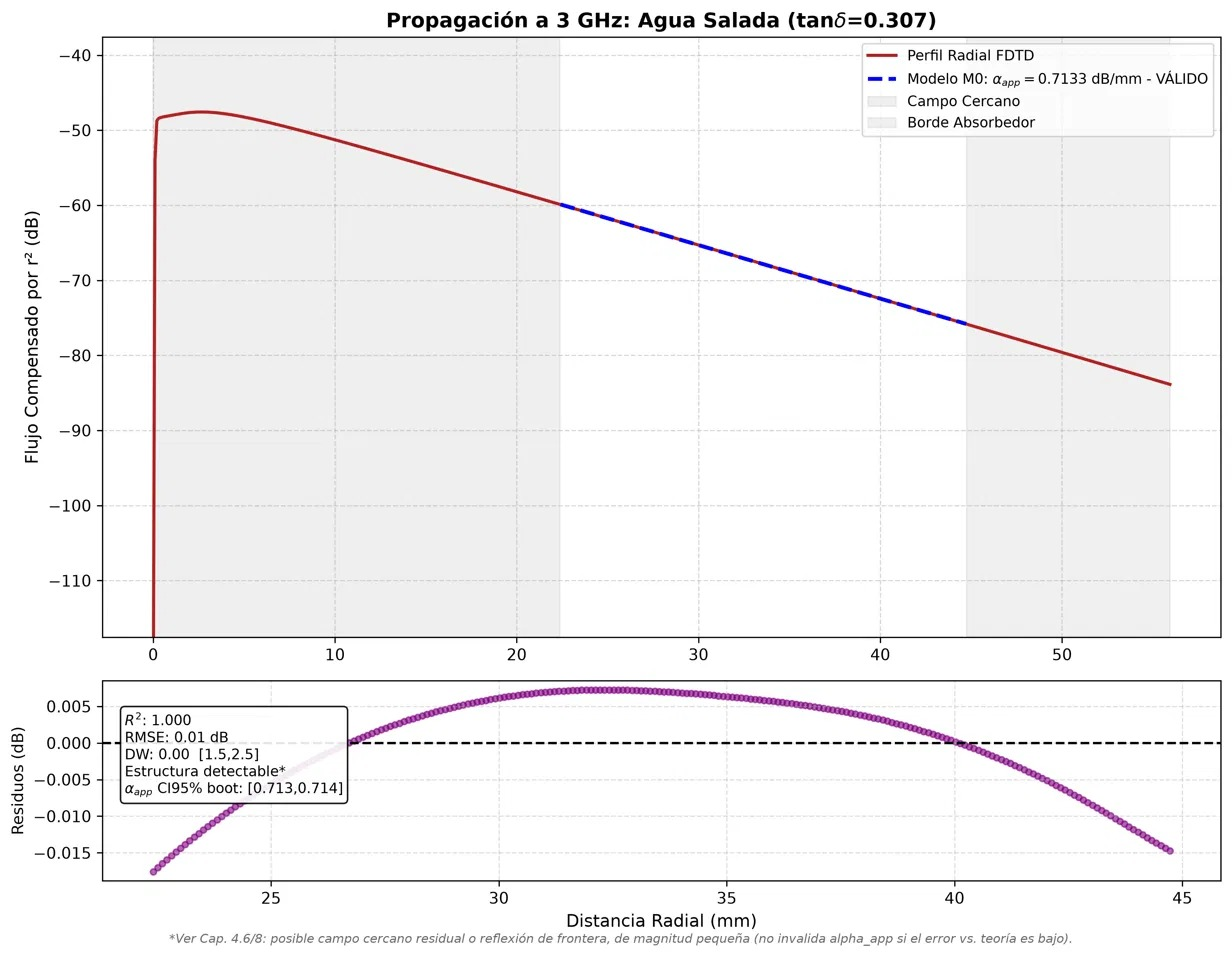
\includegraphics[width=0.83\linewidth]{figuras/Tesis_Resultado_agua_salada10px.jpeg}
\caption{Agua salada a 10 px/mm. Perfil radial y residuos de la atenuación ajustada.}\label{fig:anexo-agua-10}\end{figure}

\begin{figure}[htbp]\centering
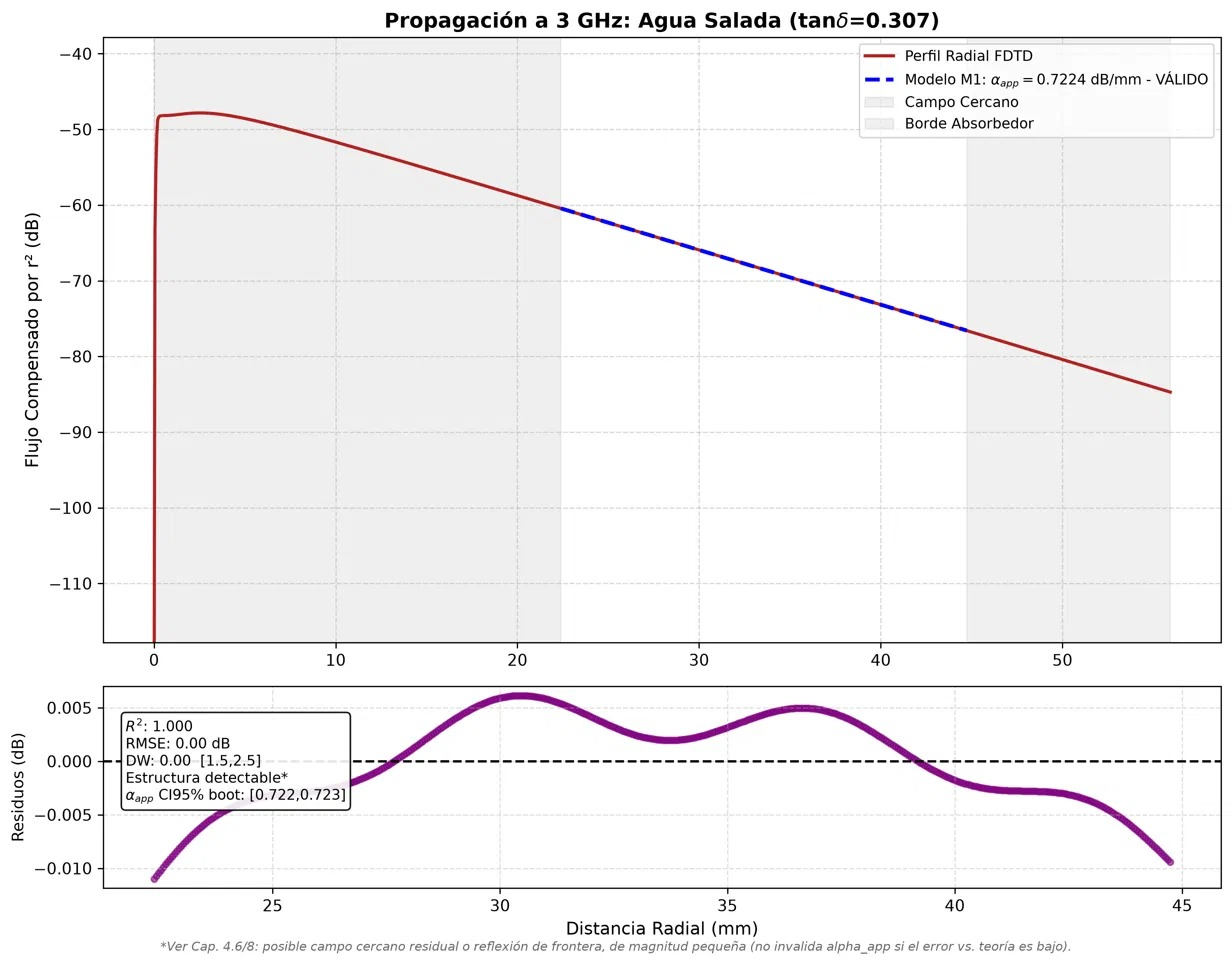
\includegraphics[width=0.83\linewidth]{figuras/Tesis_Resultado_agua_salada20px.jpeg}
\caption{Agua salada a 20 px/mm. Perfil radial y residuos de la atenuación ajustada.}\label{fig:anexo-agua-20}\end{figure}

\begin{figure}[htbp]\centering
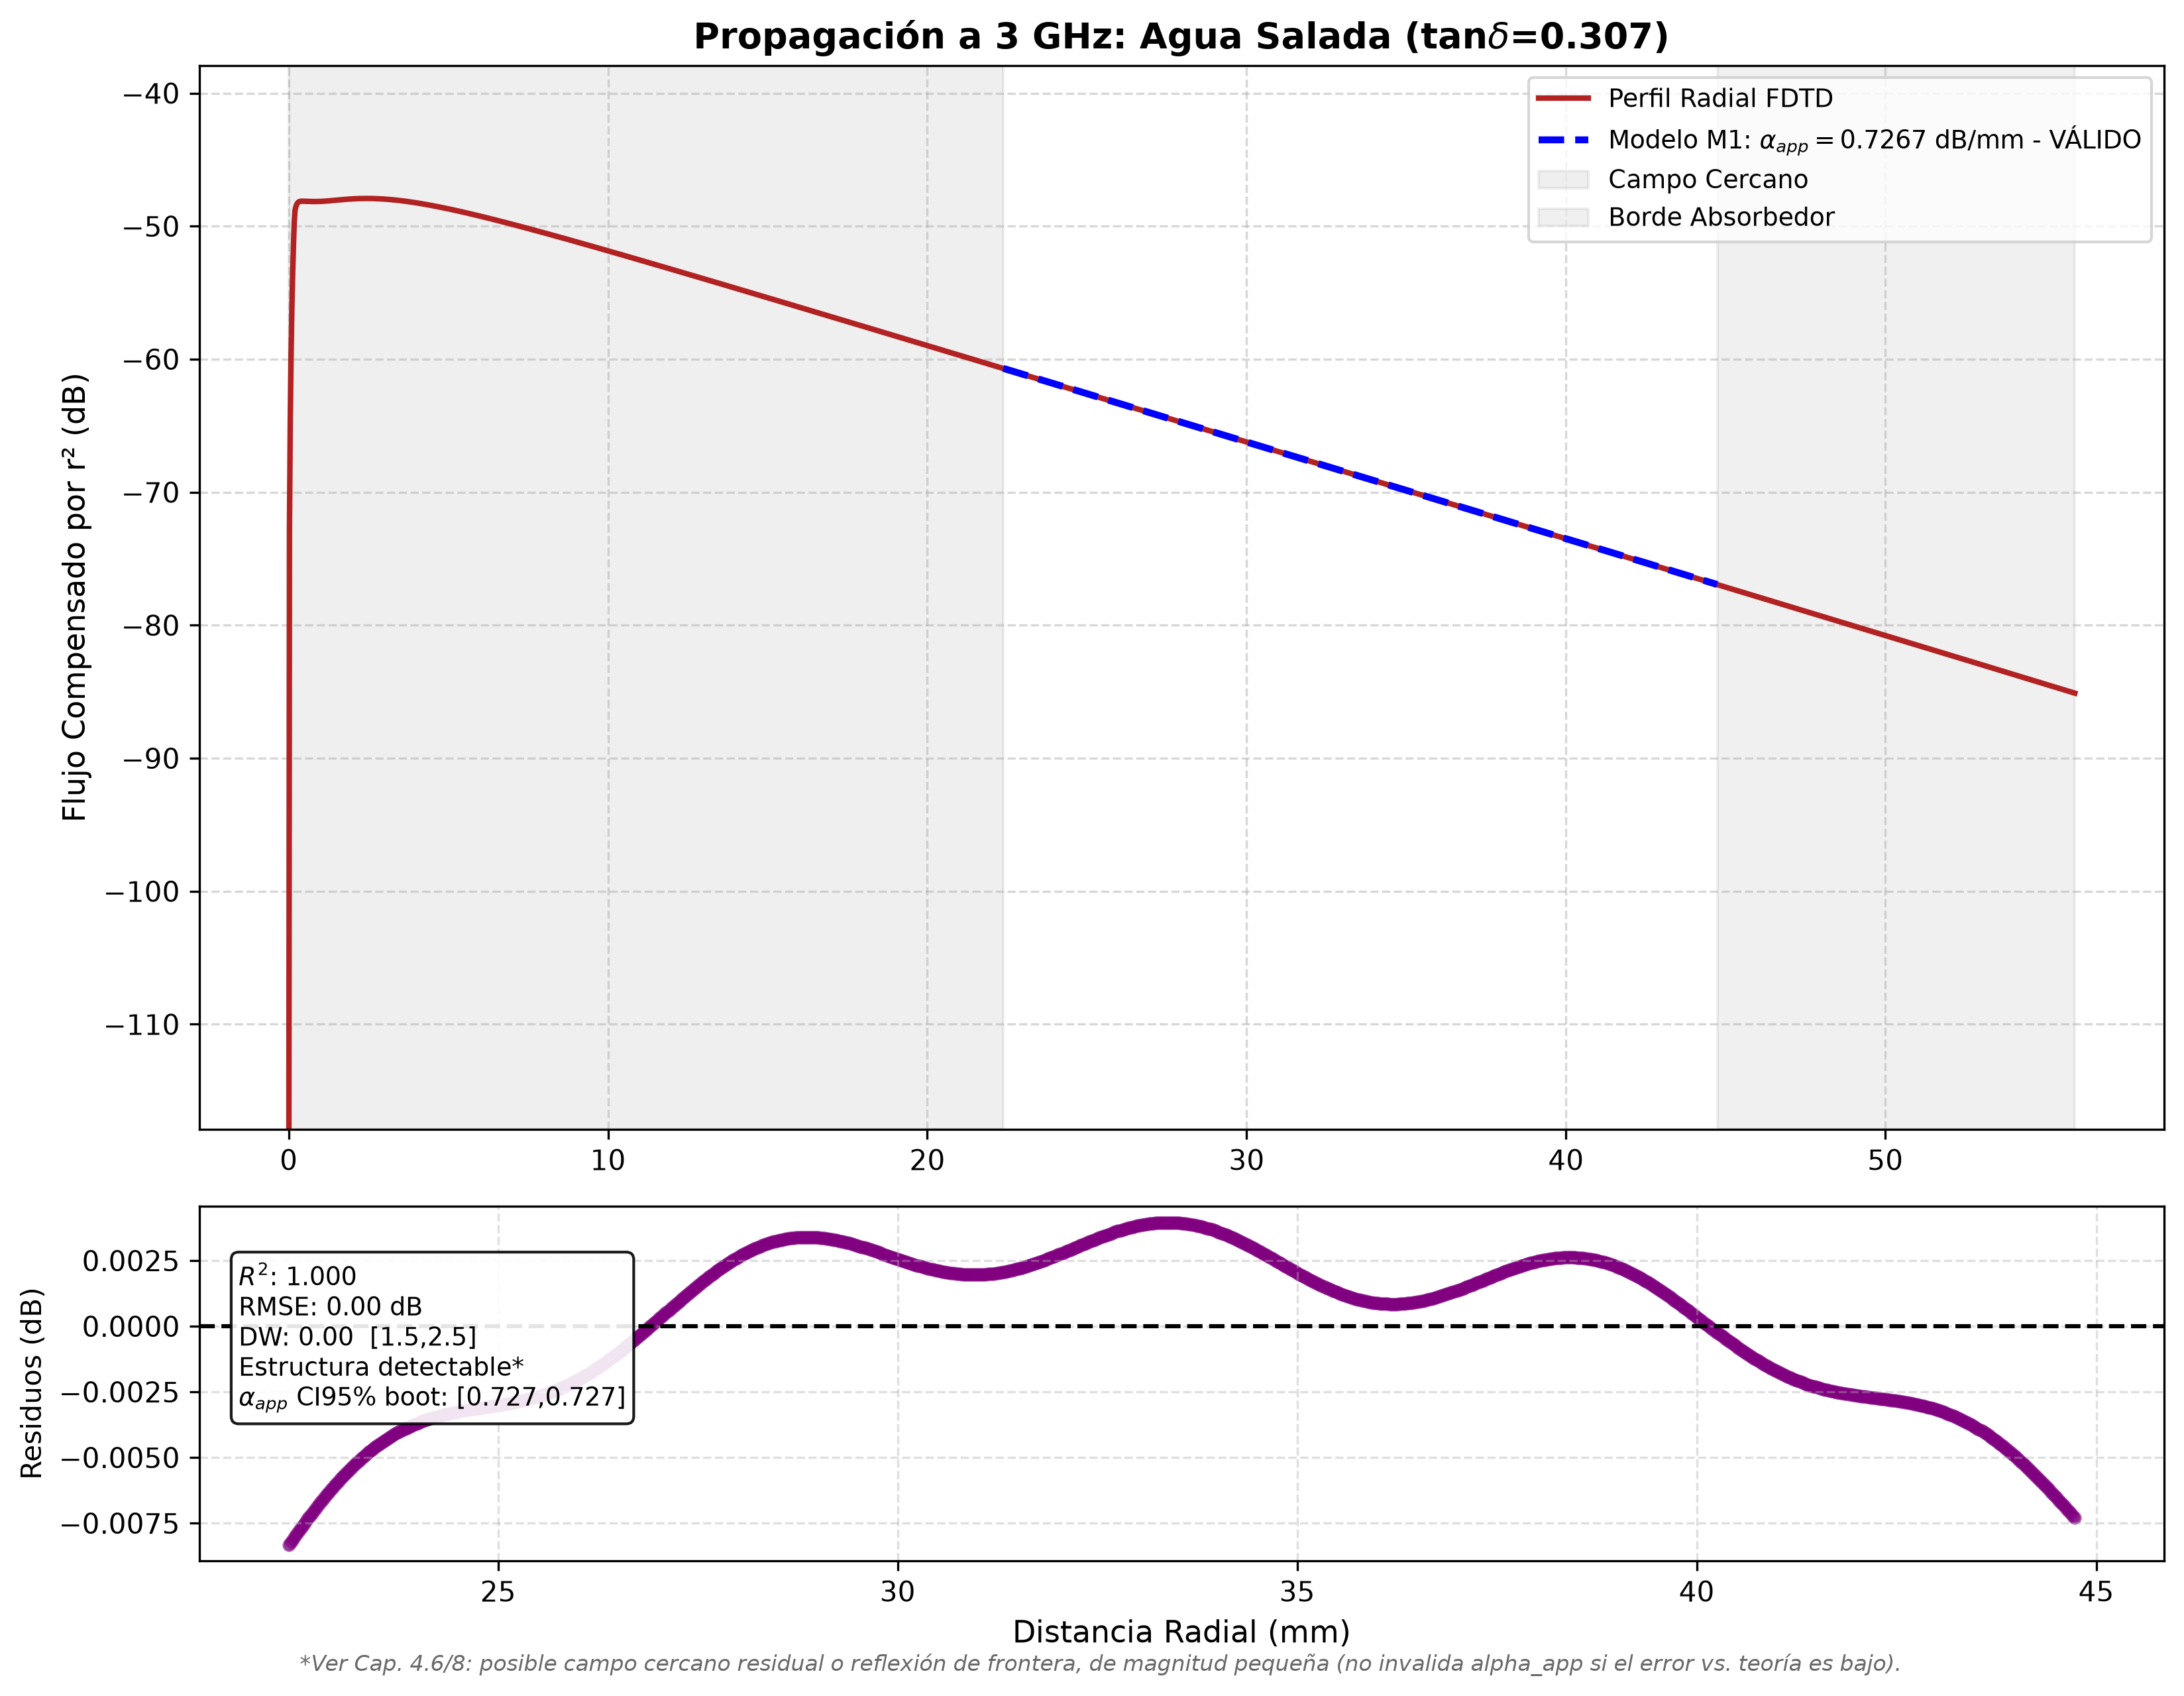
\includegraphics[width=0.83\linewidth]{figuras/Tesis_Resultado_agua_salada40px.png}
\caption{Agua salada a 40 px/mm. Perfil radial y residuos de la atenuación ajustada.}\label{fig:anexo-agua-40}\end{figure}

\begin{figure}[htbp]\centering
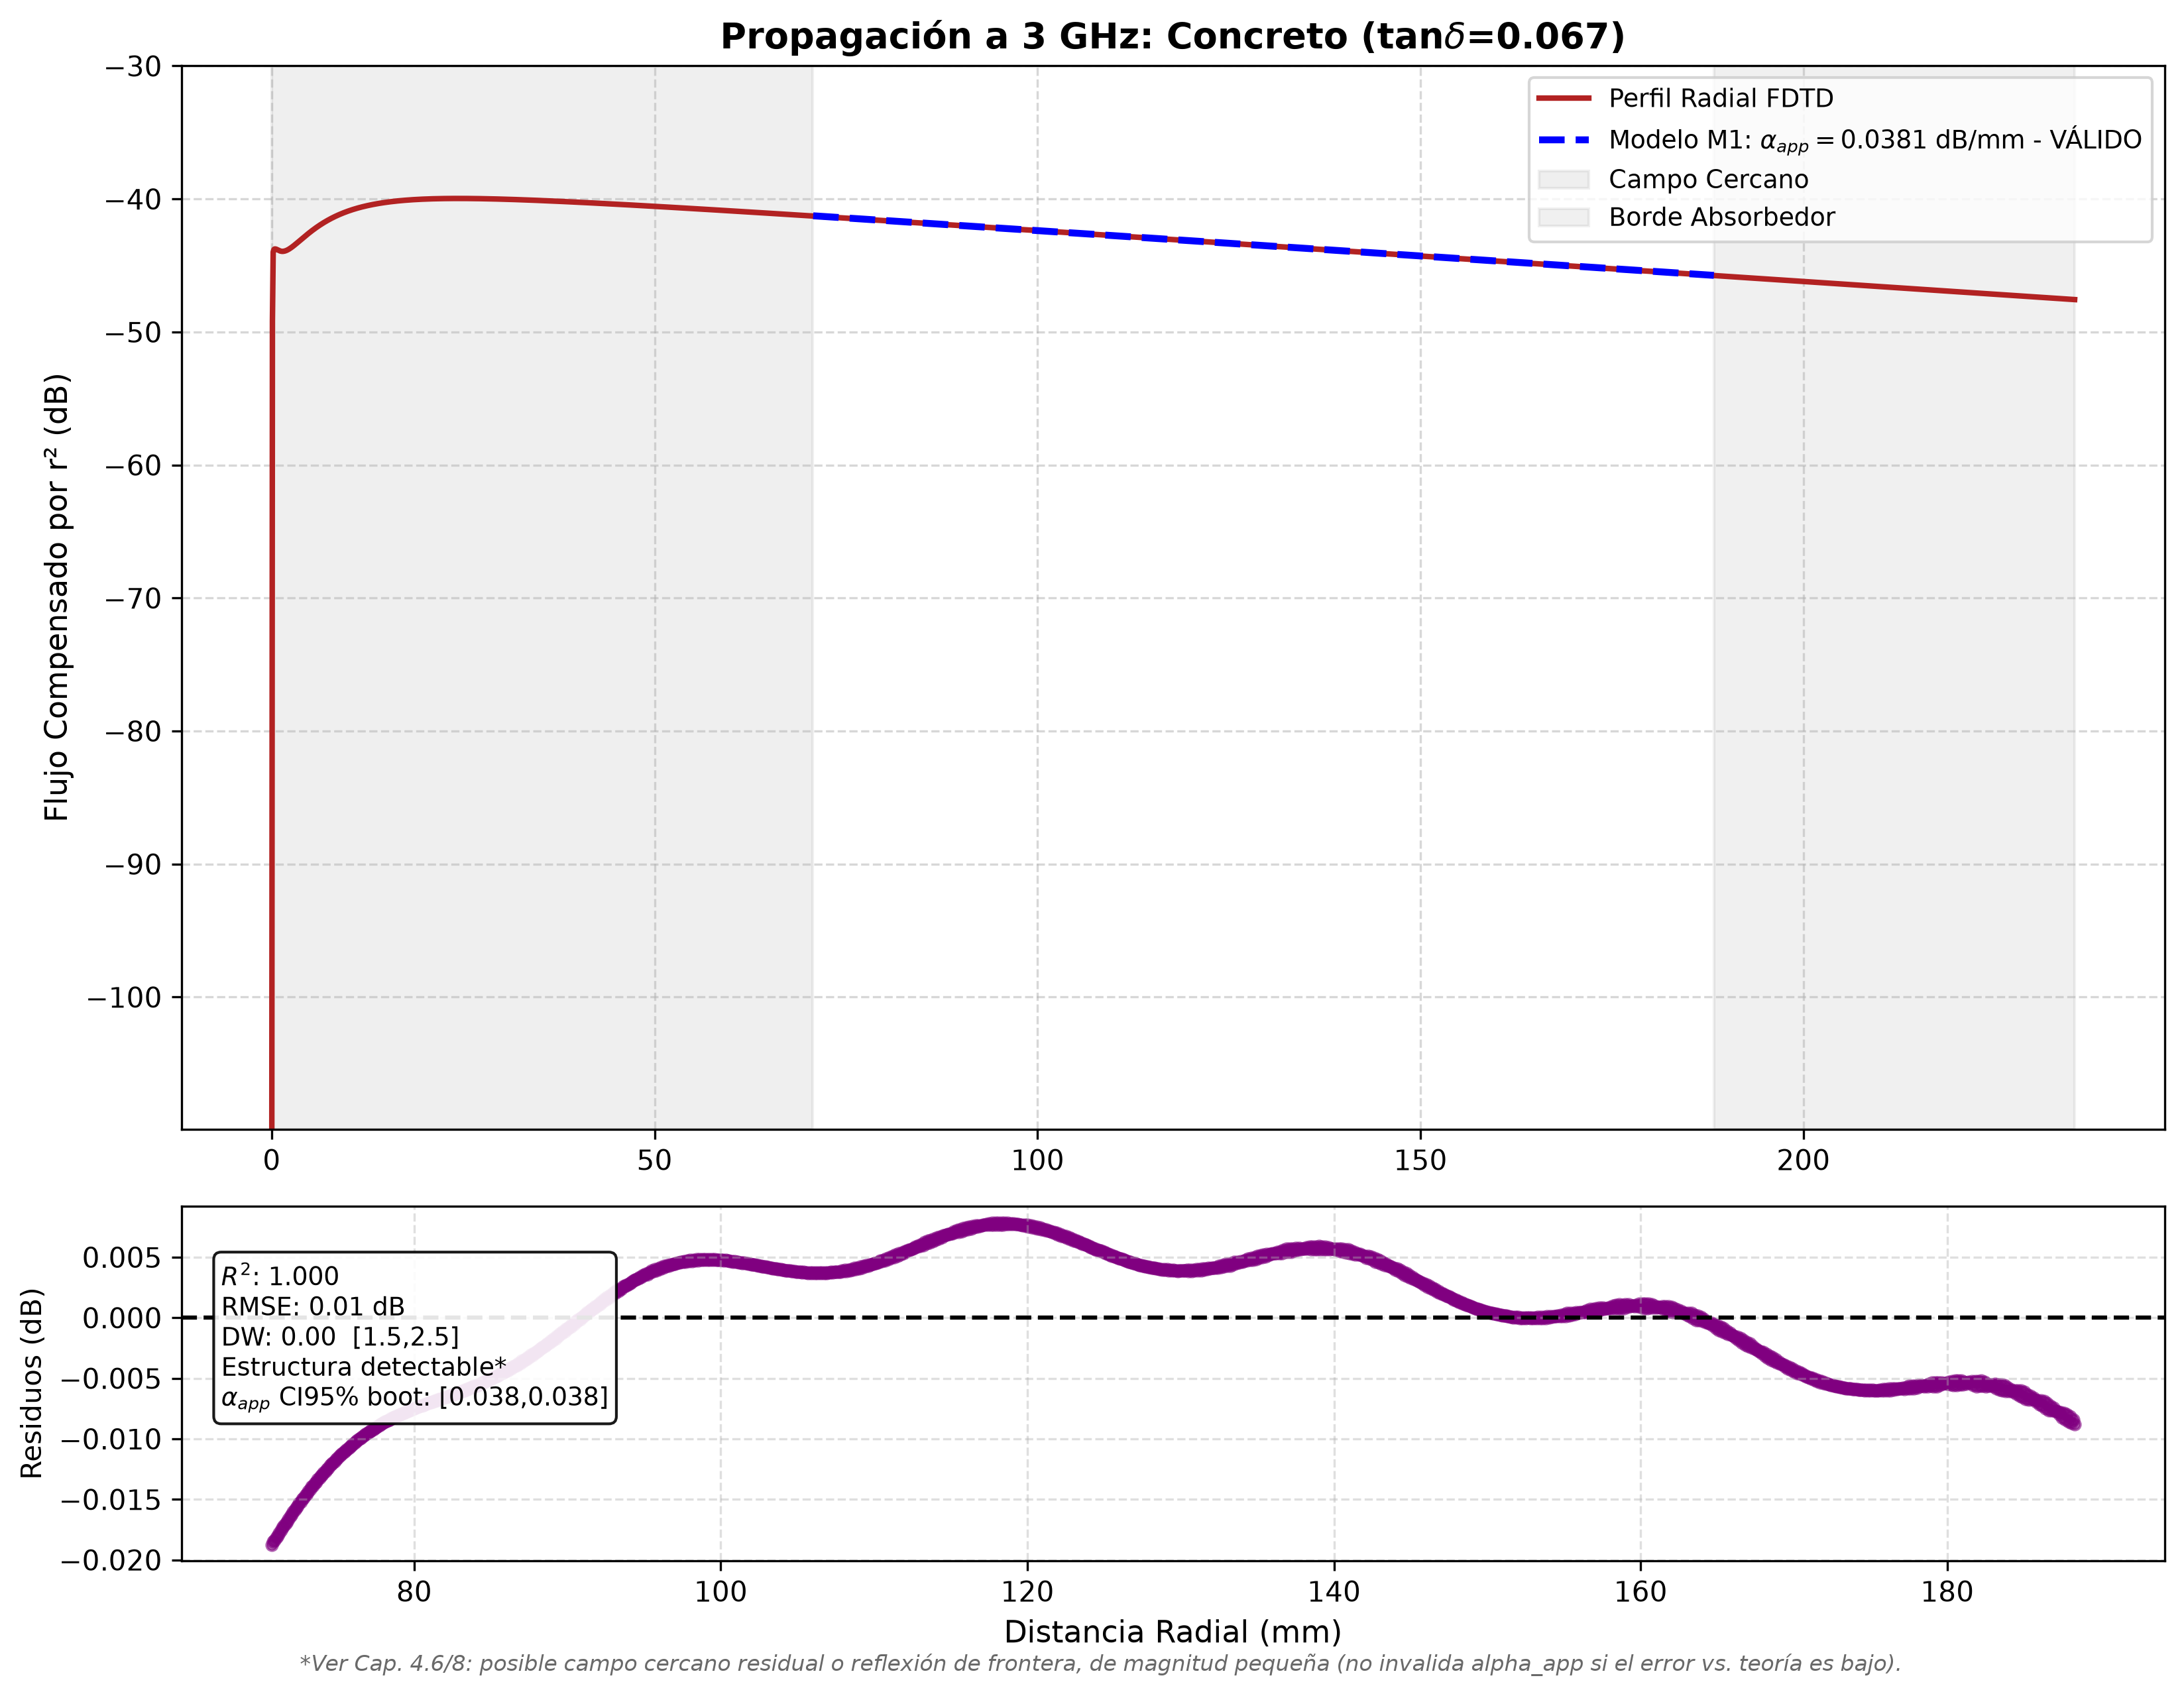
\includegraphics[width=0.83\linewidth]{figuras/Tesis_Resultado_concreto10px.png}
\caption{Concreto a 10 px/mm. Perfil radial y residuos de la atenuación ajustada.}\label{fig:anexo-concreto-10}\end{figure}

\begin{figure}[htbp]\centering
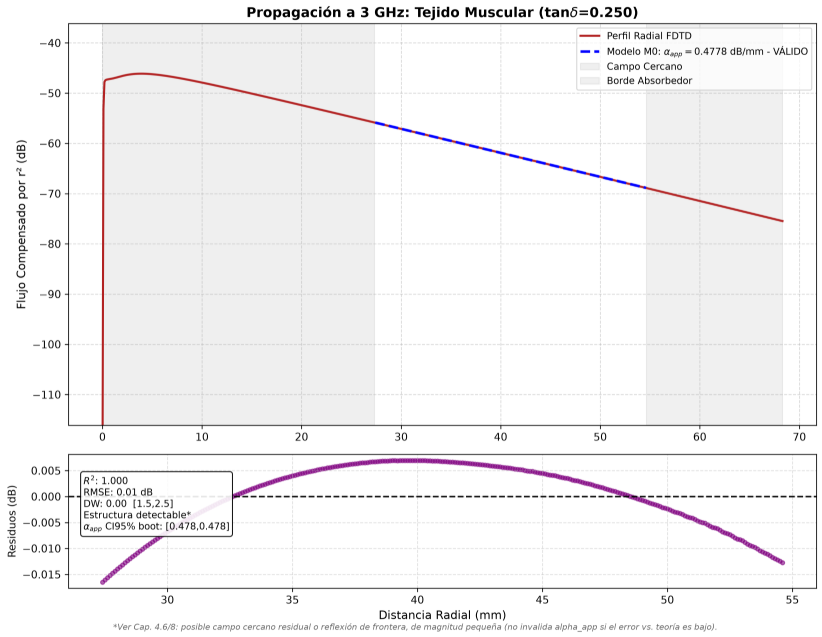
\includegraphics[width=0.83\linewidth]{figuras/Tesi_Resultados_tejido_mucular10px.png}
\caption{Tejido muscular a 10 px/mm. Perfil radial y residuos de la atenuación ajustada.}\label{fig:anexo-musculo-10}\end{figure}

\begin{figure}[htbp]\centering
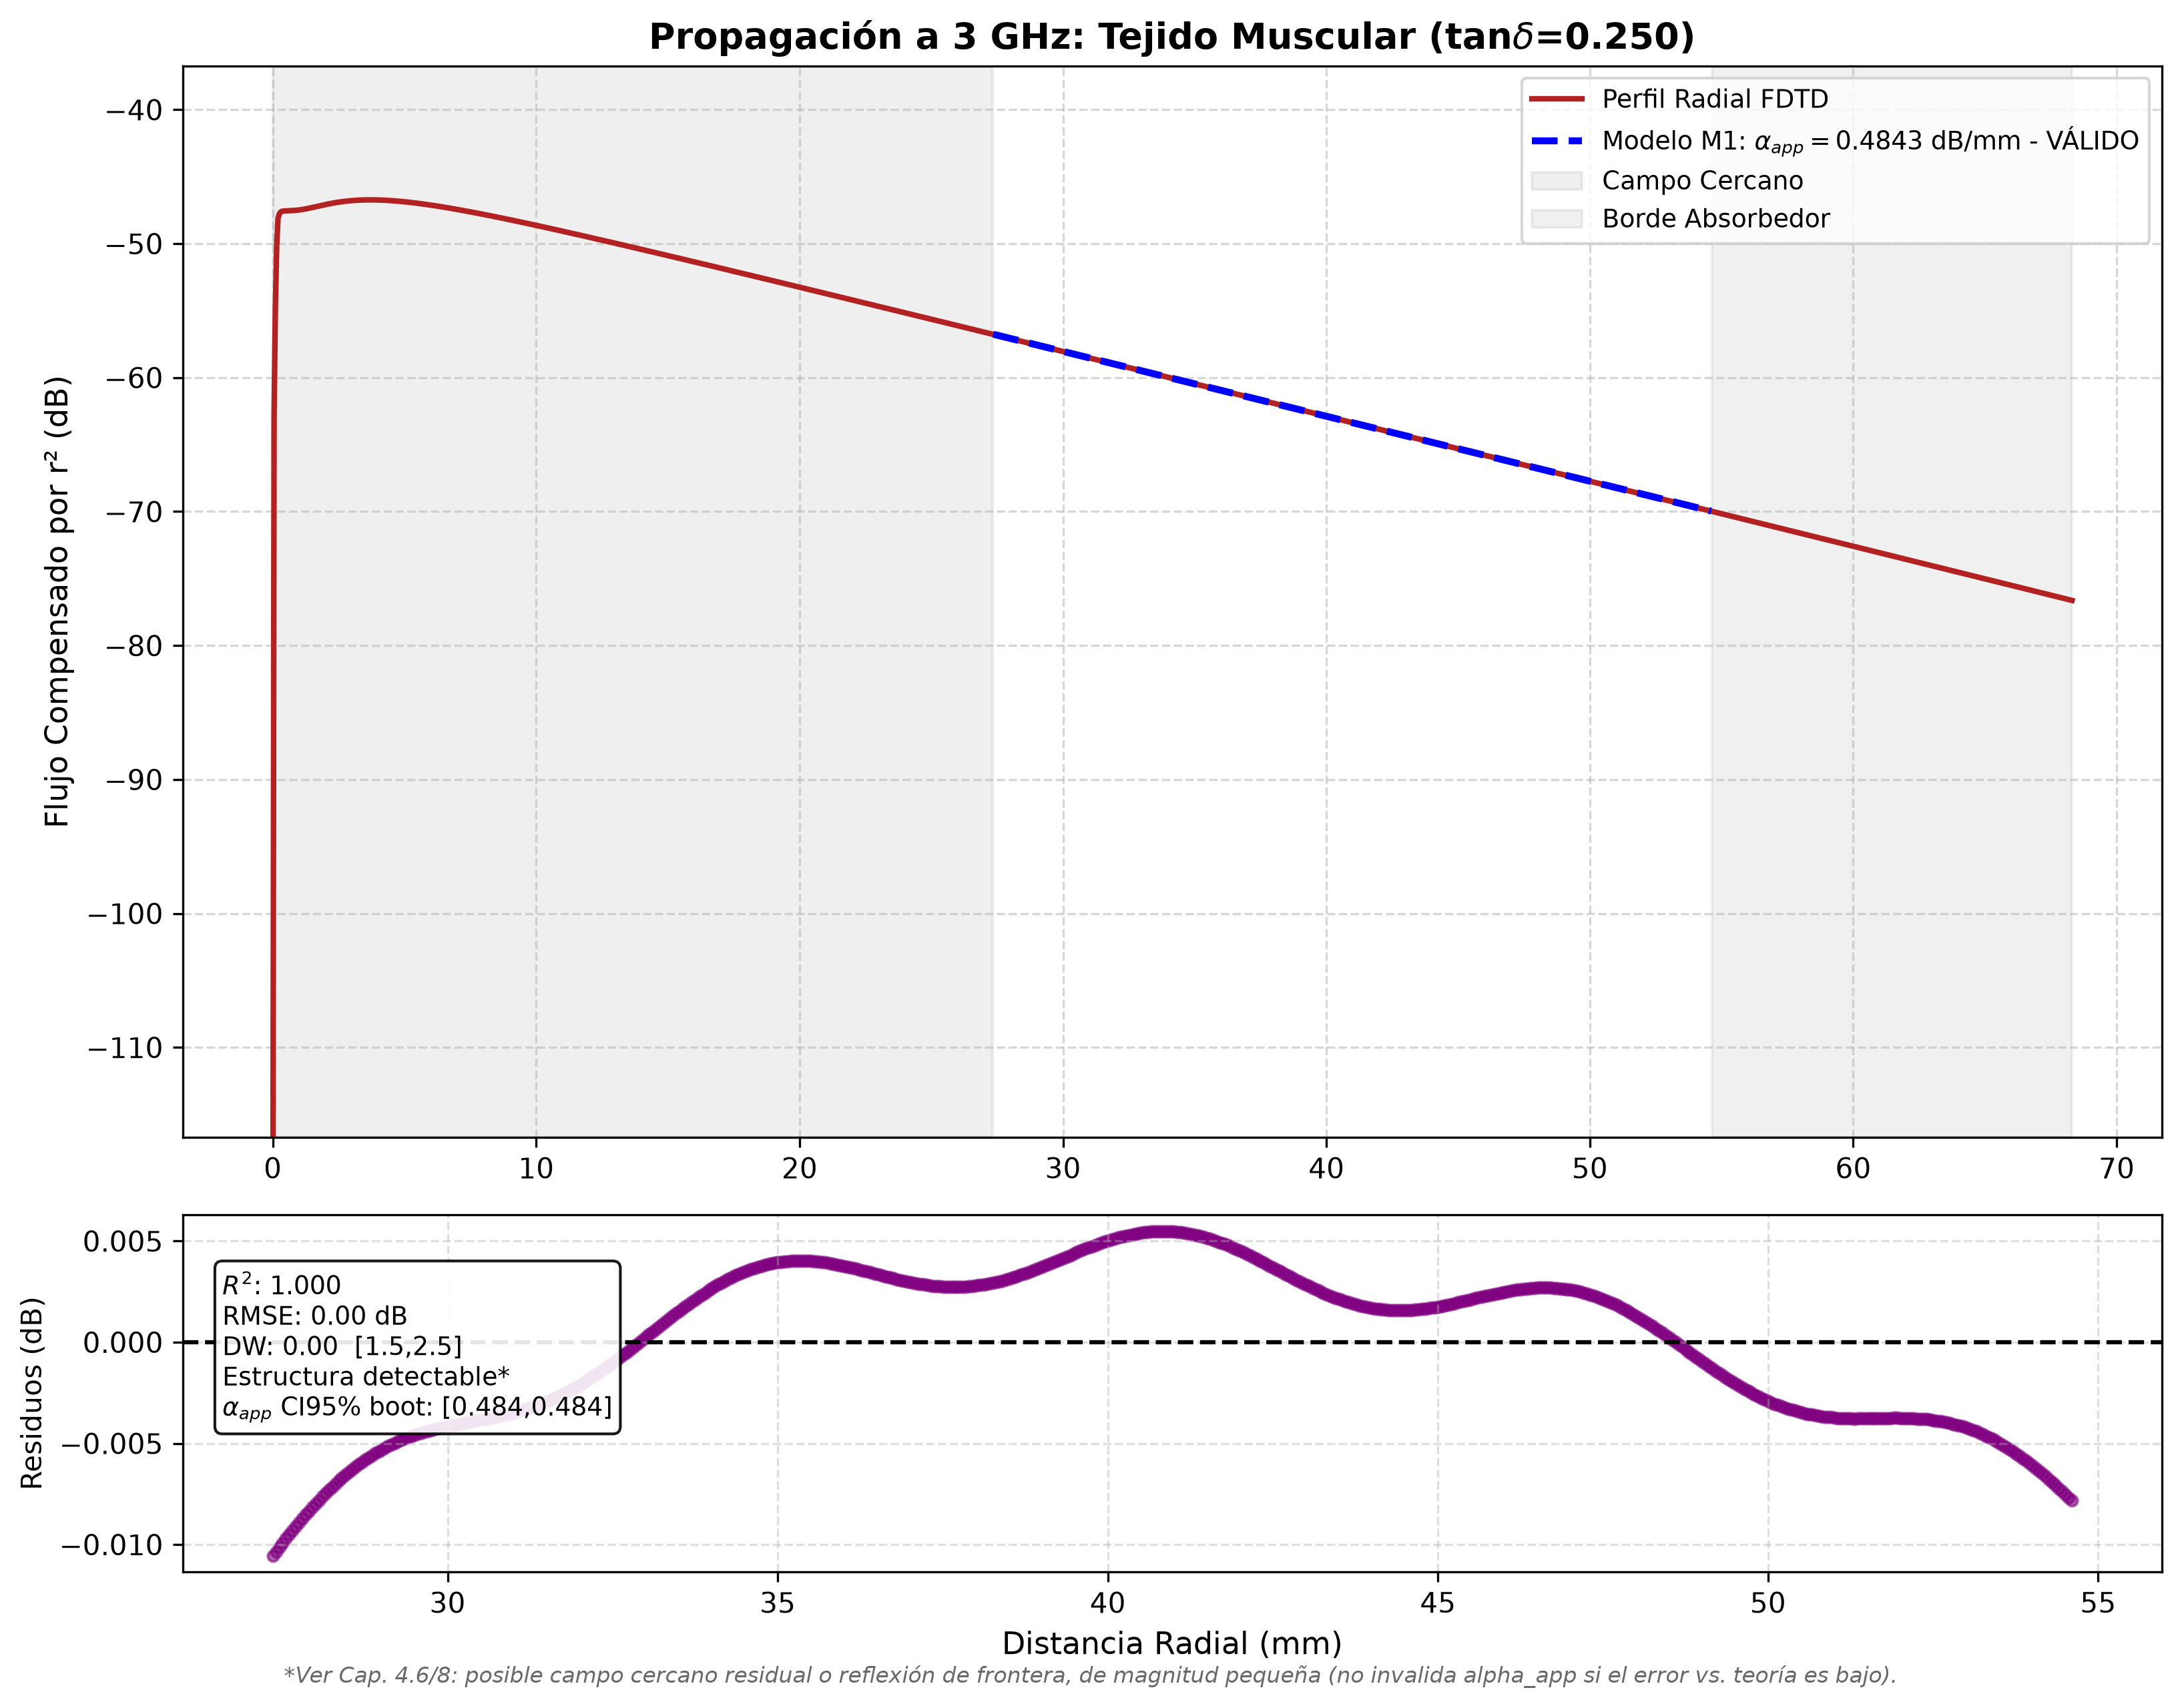
\includegraphics[width=0.83\linewidth]{figuras/Tesis_Resultado_tejido_muscular20px.png}
\caption{Tejido muscular a 20 px/mm. Perfil radial y residuos de la atenuación ajustada.}\label{fig:anexo-musculo-20}\end{figure}

	\fi
\fi

% GLOSARIO
% --------------------------------------------------------------------------------
% \ifdefined\CAPglosario
% 	\newpage
% 	\printglossary
% \fi

% LISTADO DE SÍMBOLOS
% --------------------------------------------------------------------------------
% \ifdefined\CAPsimbolos
% 	\newpage
%     \cleardoublepage\phantomsection
%     \printnomenclature
% \fi

\end{document}
